\documentclass[12pt, a4paper, oneside]{report}


\usepackage{pdfpages}
\usepackage{hyperref}
\usepackage{parskip}
\usepackage{graphicx}
\usepackage{float}
\usepackage[margin=1in]{geometry}
\usepackage{mathtools}
\usepackage{caption}
\usepackage{subfigure}
\usepackage{array}
\usepackage{verbatim}
\usepackage{pythonhighlight}
\usepackage{url}
\usepackage{listings}
\usepackage{empheq}
\usepackage{tcolorbox}
\usepackage{multirow}
\usepackage{siunitx}
\usepackage{tabularx}
% References Package
\usepackage[utf8]{inputenc}
\usepackage[english]{babel}
\usepackage[square,numbers]{natbib}
\bibliographystyle{abbrvnat}

\renewcommand{\bibname}{References}





% 自定义背景颜色
\definecolor{mybg}{RGB}{37, 148, 255}


\setlength{\parindent}{0pt}
\lstset{
	language = python,
	basicstyle = \small\ttfamily, % 基本样式 + 小号字体
	rulesepcolor= \color{gray}, % 代码块边框颜色
	backgroundcolor = \color{gray!10},
	breaklines = true, % 代码过长则换行
	numbers = left, % 行号在左侧显示
	numberstyle = \small, % 行号字体
	keywordstyle = \color{blue}, % 关键字颜色
	commentstyle =\color{orange}, % 注释颜色
	stringstyle = \color{red!100}, % 字符串颜色
	frame = shadowbox, % 用(带影子效果)方框框住代码块
	showspaces = false, % 不显示空格
	columns = fixed, % 字间距固定
}
\usepackage{xcolor}
\lstset{language=python}
\begin{document}
\rmfamily
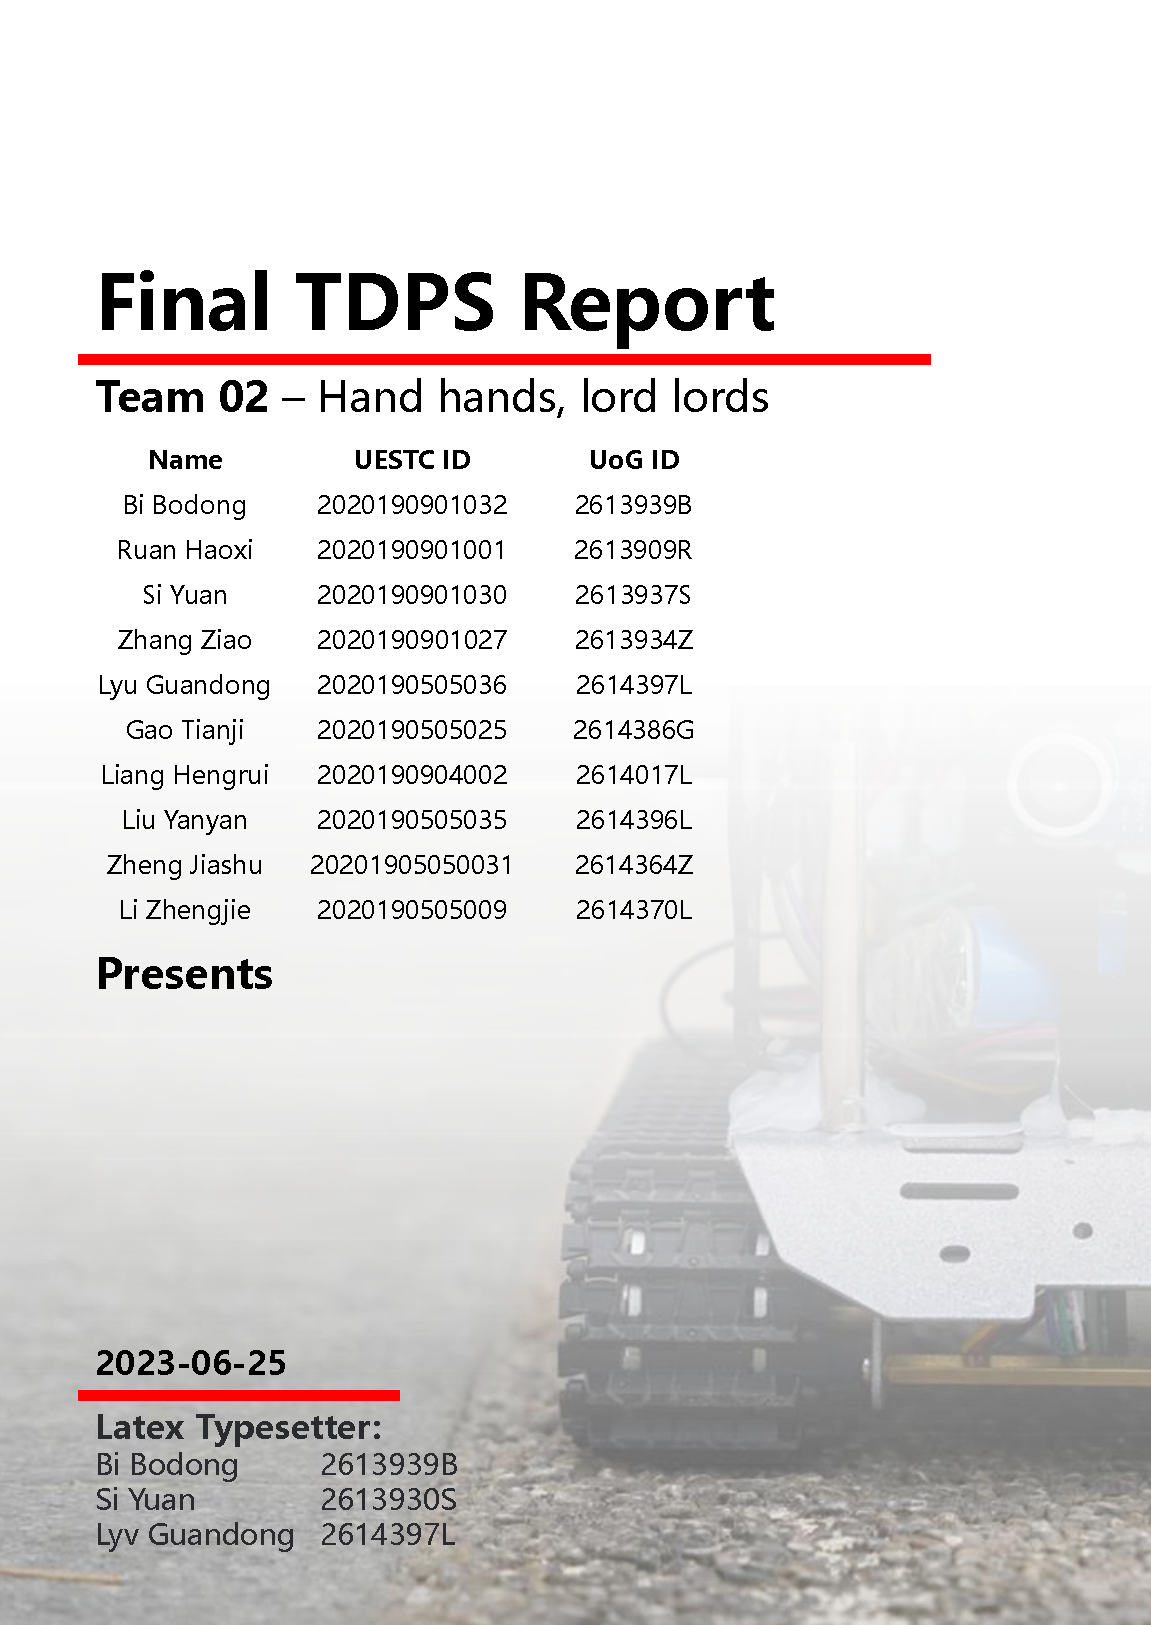
\includepdf[pages={1}]{cover.pdf}
	
\pagenumbering{Roman}

\section*{Abstract}
This report presents the design architecture and tasks of an intelligent car developed for the TDPS course, focusing on its performance in Patio 1 and Patio 2. The car is designed to navigate two lanes while completing various tasks such as recognizing arrows, releasing ping-pong balls into specific buckets, and transmitting information.

In Patio 1, the vehicle is required to follow a textured path with corners and straight sections. The camera sensor detects changes in texture and sends commands to the motor module for accurate turning. After following the path, the car must recognize a sign indicating when to turn left and cross a bridge. The bridge has specific dimensions, and upon crossing it, the vehicle needs to pass through an arch with specific specifications.

Patio 2 involves different tasks, including arrow recognition for path navigation, releasing ping-pong balls at designated locations using a releasing device, and transmitting time and group member information to a laptop via wireless serial communication. The visual sensor recognizes arrows, enabling the car to follow the correct path. The table tennis ball release mechanism employs a fan to suction and release the balls. Wireless communication is achieved using the HC-12 module controlled by the openMV's communication port.

The final design architecture of the car consists of six functional sectors: main control board, ultrasonic module, driving module, table tennis releasing module, wireless communication module, and power supply module. The main control board receives information from the openMV and other sensing modules, controlling and driving other modules. UART facilitates communication between the openMV and the STM32. The power module provides power to the vehicle, with the battery supplying 12V to the motor and a step-down module providing 5V to the STM32 and openMV. Sensing modules include the openMV camera and an ultrasonic module for obstacle detection.

In Patio 1, the car employs the openMV for visual line following and the ultrasonic module for bridge crossing. Binarization and robust linear regression are used for image processing, combined with the PID algorithm to control the motor's differential drive for line following. The ultrasonic module detects a transparent beacon, allowing the vehicle to perform a 90-degree turn before and after crossing the bridge. Ultrasonic detection of the lakeside railing stops the car's motion after passing through the archway.

In Patio 2, arrow recognition is achieved through the openMV's visual module, distance measurement and line following employ an ultrasonic module, and the ping pong ball release mechanism utilizes a fan's rotation. Wireless communication is implemented using the HC-12 module.

Overall, this report provides an overview of the intelligent car's design architecture and its capabilities in completing various tasks in Patios 1 and 2 of the TDPS course.
\newpage
\section*{Acknowledgements}
I am the group leader of team 02, Bi Bodong. Here, I would like to express my heartfelt gratitude to the teachers and classmates who have helped us throughout the TDPS project, from the beginning to the end.

Firstly, I would like to thank Professor Abdullah Al-Khalidi and Professor Oluwakayode Onireti from the TDPS project. Your lectures at the beginning of the semester provided us with direction and constructive suggestions and guidance for our project. Without your help, I would not have been able to efficiently manage the division of tasks and progress of the team throughout the entire project, which could have resulted in us being unable to assemble the car within the required time. Additionally, your introduction and requirements for the Lab Notebook also helped us smoothly conduct our experiments. With it, we were able to clearly record the progress of each experiment and plan for the next one.

Next, I would like to express my gratitude to my dedicated team members. It is through your collective cooperation, understanding of my management, and support that ensured the success of our car. Here, I would like to give special thanks and praise to several team members who have made outstanding contributions to the project.

Firstly, I want to thank Gao Tianji for his work on the motor circuitry and the logical implementation of Patio2. During the 7-day Patio2 testing period, he worked with me for over 10 hours every day in hot weather without complaining. We encountered many difficulties and unknown bugs during testing, but he faced these challenges calmly and resolutely, doing his best to solve them. In the end, we achieved an excellent Patio2 logic, where the car can correct its own path based on the railings, performing exceptionally well.

Next is Zhang Ziao, who was mainly responsible for the implementation of the ultrasonic module. He made significant contributions in both Patios and attended almost all of the 17 days of offline testing, ensuring the sensitivity and stability of our ultrasonic system.

Then, there is Si Yuan, who integrated all the components of the car. In the offline testing, his tasks were practically completed, but he still accompanied me every day, helping with various experimental debugging tasks and transporting missing parts to and from the dormitory. Without him, our progress would not have been smooth. Moreover, as my good friend, he provided me with solid emotional support during the challenging testing phase, helping me get through those difficult times.

I want to emphasize that my special thanks to these three team members does not imply that other team members did not perform well in the project. All team members completed their parts on time and with good quality, obeying my management and coordination. It's just that these three team members indeed contributed a lot to our team. In this project, our entire team collaborated, applying the knowledge and experience we have gained over our three years of university education, and ultimately achieved this proud accomplishment. I believe that even years later, when TDPS is mentioned, we will smile and reminisce about those unforgettable times.

Lastly, let me conclude our TDPS project with the slogan of my favorite YouTuber MediaStorm, "Infinite Progress!"
\begin{figure}[H]
  \centering
  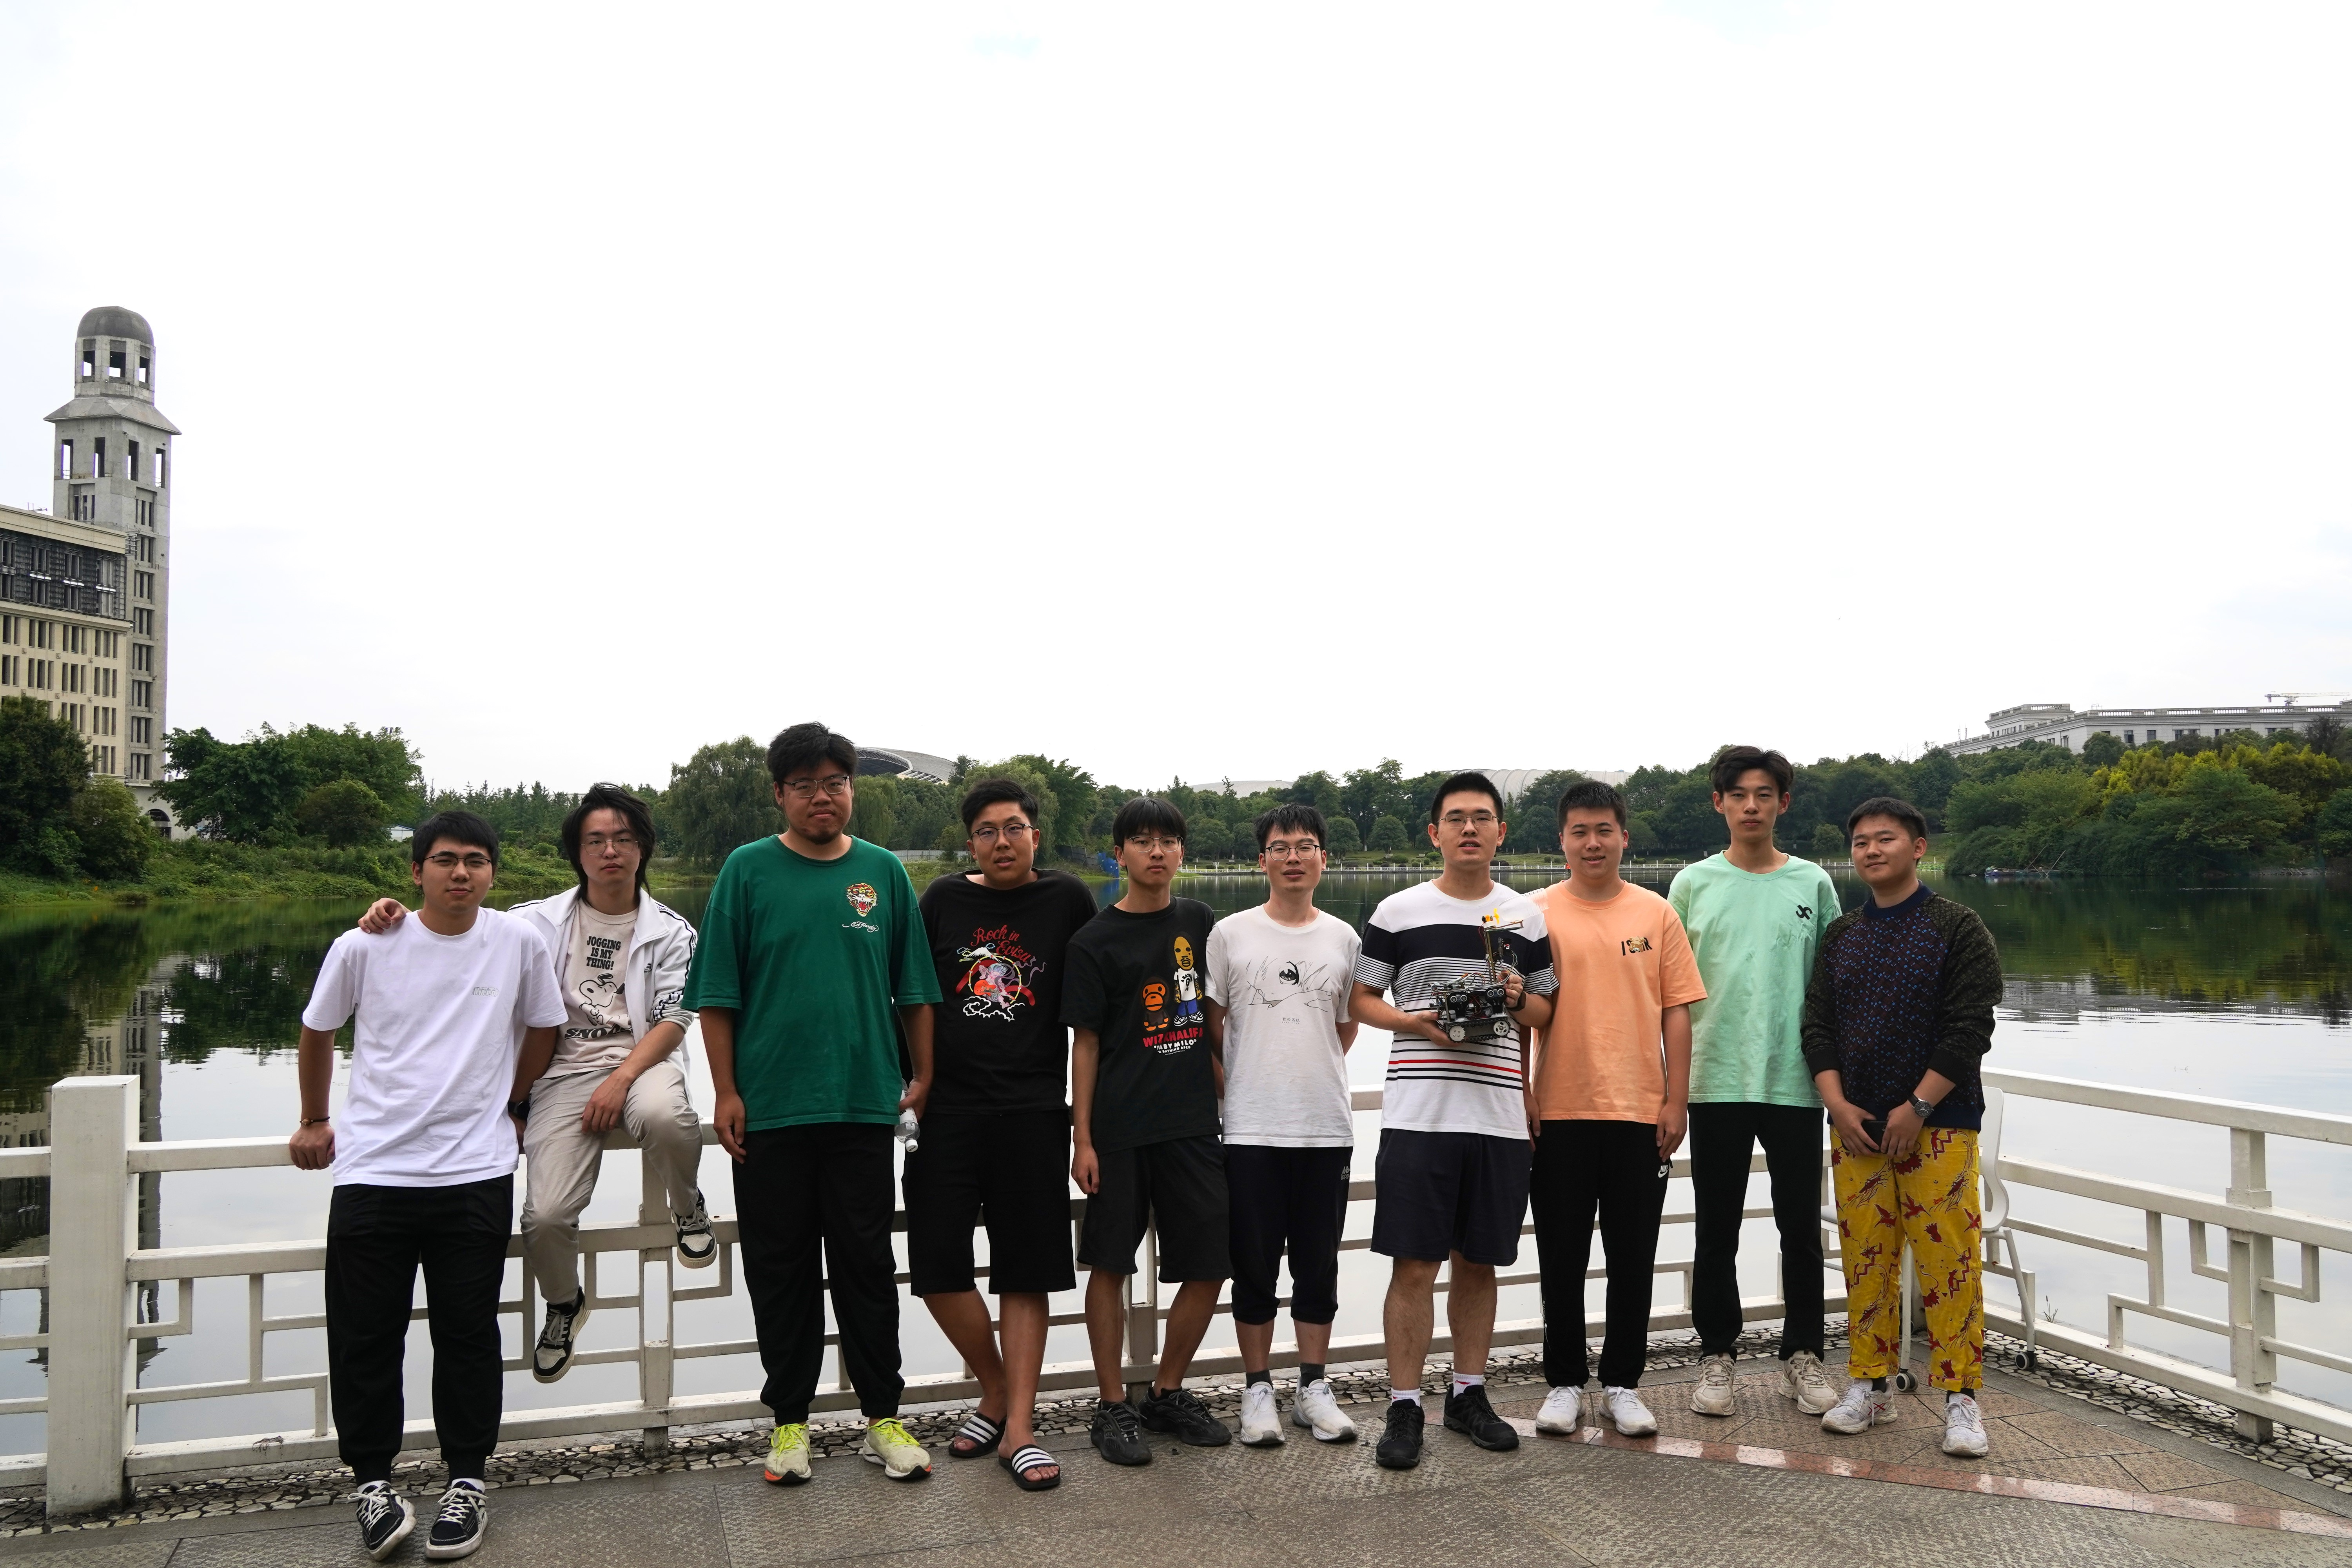
\includegraphics[width=1\textwidth]{pic/Thanks/team02.jpg}
  \label{fig:team02}
\end{figure}

\begin{figure}[H]
  \centering
  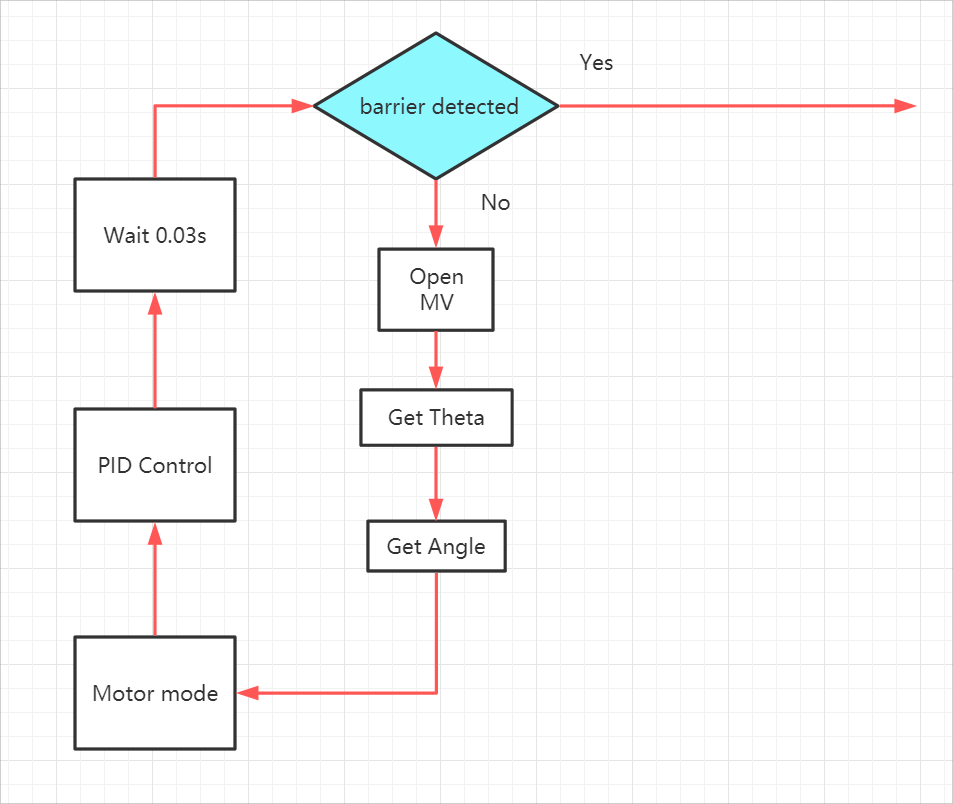
\includegraphics[width=1\textwidth]{pic/Thanks/2.JPG}
  \label{fig:team02-2}
\end{figure}

\newpage
\section*{Individual Guidance}
In this section, we will introduce the roles and responsibilities of each member in our team. \textbf{Spectrum of Duty} has been set up as a hyperlink that you can click on directly to access.
\vspace{\baselineskip}

\colorbox{yellow}{\textbf{Member 1: Bi Bodong 2613939B} }
\begin{tcolorbox}
\textbf{Spectrum of Duty:} 
\hyperref[sec:Tracing]{\textcolor{mybg}{Track Recognition and Tracing}}/
\hyperref[sec:Pitch]{\textcolor{mybg}{Pitch Function of OpenMV}}

\textbf{Latex Typesetter}
\end{tcolorbox}

I am the team leader, and I am responsible for the development of the line-tracing module based on OpenMV and the camera pitch module. My primary task is situated in Patio 1, which involves guiding the car to follow the designated path in Patio 1, navigate through several turns, and ultimately reach the position of the bridge. In addition to this, the pitch module I have developed provides a feasible solution for quick transitions between Patios, facilitating smooth switching between different sections.
\vspace{\baselineskip}

\colorbox{yellow}{\textbf{Member 2: Si Yuan 2613937S} }
\begin{tcolorbox}
\textbf{Spectrum of Duty:} 
\hyperref[sec:Hardware]{\textcolor{mybg}{Hardware Design}}

\textbf{Latex Typesetter}
\end{tcolorbox}

I am responsible for the overall construction of the vehicle structure. My tasks include designing the vehicle as a whole, selecting the chassis, and choosing the components for the vehicle. Through field investigations and testing, I ensure that the vehicle can operate successfully in both patios. Additionally, I am in charge of arranging different components in appropriate positions on the upper and lower layers, laying a solid hardware foundation for the successful completion of the tasks.

\vspace{\baselineskip}


\colorbox{yellow}{\textbf{Member 3: Gao Tianji 2614386G} }
\begin{tcolorbox}
\textbf{Spectrum of Duty:} 
\hyperref[sec:CD]{\textcolor{mybg}{Circuit Drive}}/
\hyperref[sec:itm]{\textcolor{mybg}{Inertial Measurement Unit}}

\textbf{Co-Author of Chapter 4 Patio 2}
\end{tcolorbox}
I was responsible for the writing of the control program and the development of some hardware modules at software level. My main task was to write all the main control code for the Patio 2 in the microcontroller, which was used to control the rover for all its tasks. In addition, I developed the IMU (Inertial Measurement Unit) module and the code level implementation for controlling the rover steering and I was also involved in the development of the software side of the motor drive, i.e. how to control the motor with the master program in the MCU.
\vspace{\baselineskip}

\newpage
\colorbox{yellow}{\textbf{Member 4: Zhang Ziao 2613934Z} }
\begin{tcolorbox}
\textbf{Spectrum of Duty:} 
\hyperref[sec:SR-04]{\textcolor{mybg}{Ultrasonic Distance Detection}}

\textbf{Co-Author of Chapter 4 Patio 2}
\end{tcolorbox}
I am responsible for the development of the HC-SR04 ultrasonic sensor module. My task involves configuring the ultrasonic sensors on the rover to obtain necessary distance data in different scenarios. In Patio 2, I utilized the front sensor and two right sensors to guide the rover to the task location where it should accurately throw the ball into the bin. The front sensor also assisted the rover in determining when to ascend and and what to do after descending the bridge in Patio 1. Additionally, I have contributed to locating the beacons in Patio 1 and Patio 2 because they were detected by the ultrasonic sensors, ensuring the successful execution of the rover's tasks.
\vspace{\baselineskip}

\colorbox{yellow}{\textbf{Member 5: Lyu Guandong 2614397L} }
\begin{tcolorbox}
\textbf{Spectrum of Duty:} 
\hyperref[sec:itc]{\textcolor{mybg}{Communication between Boards}}

\textbf{Latex Typesetter}
\end{tcolorbox}
In this project, my role as a team member focused on establishing effective communication between the STM32 and OpenMV boards. This involved understanding project requirements, integrating hardware, selecting appropriate communication protocols, implementing software components, ensuring data synchronization, testing and debugging, documenting my work, and collaborating with team members. My contribution significantly contributed to the seamless and reliable communication between the boards, enhancing the overall functionality and performance of the line tracing car.
\vspace{\baselineskip}

\colorbox{yellow}{\textbf{Member 6: Liang Hengrui 2614017L} }
\begin{tcolorbox}
\textbf{Spectrum of Duty:} 
\hyperref[sec:PCB]{\textcolor{mybg}{Printed Circuit Design (PCB)}}
\end{tcolorbox}
I took charge of our smart vehicle's printed circuit board (PCB) design. This work mainly contains the design of modules schematics, the design of PCB layout and passive components assembling. Then, cooperated with teammates combining the complete PCB with the physical supporting structure to provide stable electric power and signal connection between modules. In addition, I defined the Gantt Chart based on our group plan at the initial project stage.
\vspace{\baselineskip}

\colorbox{yellow}{\textbf{Member 7: Zheng Jiashu 2614397L} }
\begin{tcolorbox}
\textbf{Spectrum of Duty:} 
\hyperref[sec:CD]{\textcolor{mybg}{Circuit Drive}}/
\hyperref[sec:tb]{\textcolor{mybg}{Table Tennis Ball Release Module}}
\end{tcolorbox}
I was responsible for task 2 of the Patio 2, i.e. designing, building, connecting and assembling the table tennis ball release device. As the device involves the use of a motor drive, I have also designed the motor drive module circuit for the TB6612 chip, which is used for the control of all the motors. As the motor drive is part of the power supply system, I have also been involved in designing the supply voltage step-down module using a voltage regulator triode.
\vspace{\baselineskip}

\colorbox{yellow}{\textbf{Member 8: Ruan Haoxi 2613909R} }
\begin{tcolorbox}
\textbf{Spectrum of Duty:} 
\hyperref[sec:Arrow]{\textcolor{mybg}{Arrow Recognition}}
\end{tcolorbox}
I am responsible for the development and implementation of the arrow identification based on OpenMV. This task is in Patio 2, which involves utilizing the camera of OpenMV to identify the direction of a arrow on the road and send messages to the rover, so that it can head to the correct direction. As for the implementation of this module, I have considered many methods and finally used template matching based on OpenMV to achieve this task. I have conducted some experiments and tried many turns to test whether this method has high reliability, and optimized the methods for several times to ensure it has a high accuracy in the identification of the arrow.
\vspace{\baselineskip}

\colorbox{yellow}{\textbf{Member 9: Li Zhengjie 2614370L} }
\begin{tcolorbox}
\textbf{Spectrum of Duty:} 
\hyperref[sec:hc12]{\textcolor{mybg}{Message Wireless Transmission}}
\end{tcolorbox}
I am responsible for completing wireless communication. My task is to configure the HC-12 module to send the desired message when the rover achieves at the designated region. In the Patio 2, I configure the OpenMV the RTC module to obtain the time information and give an activate signal as the rover arrives at the designated location to accomplish the wireless communication between PC terminal and OpenMV by utilizing two HC-12 modules.
\vspace{\baselineskip}

\colorbox{yellow}{\textbf{Member 10: Liu Yanyan 2614396L} }
\begin{tcolorbox}
\textbf{Spectrum of Duty:} 
\hyperref[sec:PID]{\textcolor{mybg}{PID Control}}/
\hyperref[sec:add]{\textcolor{mybg}{Angle and Direction Discrimination}}

\textbf{Author of Chapter 4 Patio 1}
\end{tcolorbox}
In this project, I am mainly responsible for the development of Patio1. My task involves designing an algorithm to identify the angle between the rover’s movement and the line of the road, and adjusting the operation of motor based upon the results. In this process, I wrote programme on application of PID control method, and found out the most effective parameters according to many tests and comparisons. Finally, I am responsible for integrating the functions of all unit elements to make the rover able to complete task 1.
	
\tableofcontents
\listoffigures
\listoftables

\chapter{Introduction}
\pagenumbering{arabic}
\section{Background}
In TDPS, we are tasked to design a car capable of completing three different tasks in both Patio 1 and Patio 2. TDPS is a course aimed at having students design an intelligent car as a team. The intelligent car is required to recognize two lanes and navigate on them, while completing tasks along the way. These tasks include arrow recognition, releasing ping-pong balls into specific buckets, and transmitting information.
\section{Task Objectives}
\begin{itemize}
    \item Autopilot: control Rover without external command
    \item Intelligent path recognition: the ability to discover and track ground paths
    \item Ultrasonic detection: able to identify the location of beacon and terminal arch
    \item Arrow recognition: able to recognize the arrow
    \item Release table tennis: can release table tennis to the bin
    \item send message: able to send messages to the control terminal at an appropriate position
\end{itemize}
    
\subsection{Patio 1}
For patio 1, there are totally three tasks needed to be completed. 
Firstly, the vehicle should recognize the vein and follow the textured path which consists of several corners and several straight sections. The camera sensor will be utilized to discriminate the change of the texture when at the turning corners and the microcontroller unit is expected to send the corresponding command to motor module in order to guide the vehicle turn correctly. 
After completing the task of following the path, the vehicle should recognize the sign offering the message that when to turn left and go across the bridge. The bridge is approximately 0.45m in width and the length is 2.2m around. 
After crossing the bridge, the rover is expected to go through the arch which has a certain specification. 

\subsection{Patio 2}
As for patio 2, there are also three tasks in total.
the rover is required to recognize the different shapes that are corresponding to different commands which depends on a visual sensor. Only recognizes the shape correctly could the rover follow the correct path and arriving at the required destination. 
Later, the rover should release table tennis ball at the designated location as expectancy. To complete this task, a table tennis ball releasing device will be utilized. 
The last task is to transmit a signal of current time and some information of group members to the laptop. HC-12 wireless serial communication will be used to complete this task which is under control of communication port of an openMV.

	
\chapter{Proposed Design}

The final design architecture of the rover consists of six functional sectors: main control board module, ultrasonic module, driving module, table tennis releasing module, wireless communication module and power supply module. Their relationships and connections are depicted in Gantt Chart. The basic logic of the design is that the OpenMV and other sensing modules send information to the main control board, which in turn controls and drives other modules. UART serves as the communication protocol between the OpenMV and the STM32. In our design, the power module serves as the core of the rover, responsible for providing power to the vehicle. The battery can output 12V directly for driving the motor, whereas the STM32 and OpenMV need to be powered by a step-down module capable of stepping down the 12V voltage to 5V. The sensor modules used in the vehicle include the built-in camera of OpenMV and an ultrasonic module (HC-SR04). They are capable of detecting obstacles and responding quickly. The second part, is the STM32, which has sufficient processing power to handle various computational tasks. The motor section is responsible for driving the entire vehicle. In this section, the 12V output is first connected to a motor driver device and then separately connected to two motors.

\begin{figure}[H]
  \centering
  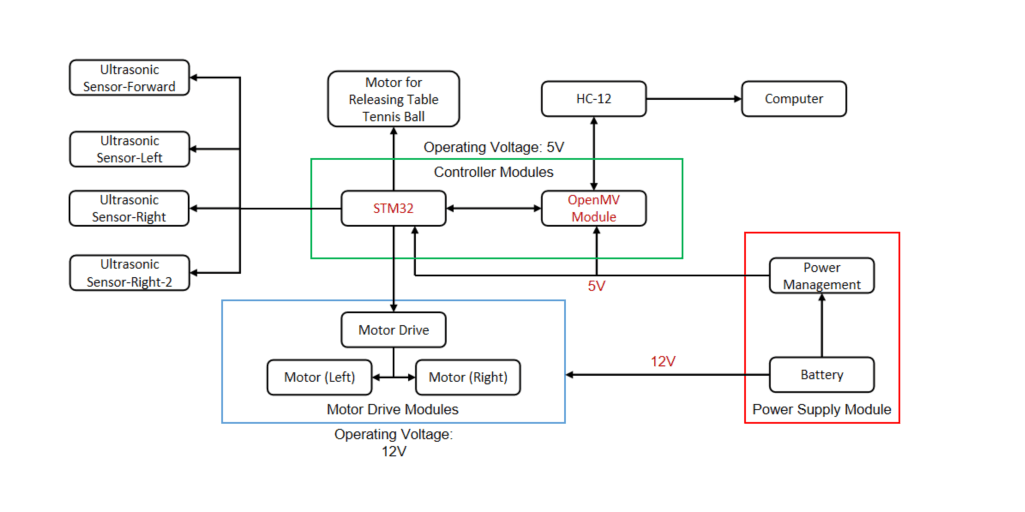
\includegraphics[width=0.95\textwidth]{pic/Proposed Design/Structure of The Rover.png}
  \caption{Structure of The Rover}
  \label{fig:Structure of The Rover}
\end{figure}

	
\section{General solutions}
	
\subsection{Patio 1 solution}
In Patio 1, the main tasks include visual line following and bridge crossing. We decided to use OpenMV for visual patrolling, which involves image processing, binarization to obtain grayscale images, and robust linear regression. Combined with the PID algorithm, we control the motor's differential drive to enable the vehicle to follow the line.

$$
J^{\text {dark }}(k)=\min _{c \in\{r, g, b\}}\left(\min _{x \in w_k} J^c(x)\right) \approx 0
$$

For the bridge crossing task, we chose to use an ultrasonic module for detection. We placed a transparent beacon at the turning point before the bridge, which allows us to achieve ultrasonic detection without interfering with visual line following. Once the vehicle receives the ultrasonic detection information, it performs a 90-degree turn. After crossing the bridge, we use another beacon to guide the vehicle in completing another 90-degree turn. Finally, the vehicle stops its motion upon ultrasonic detection of the railing at the lakeside, right after passing through the archway.

\subsection{Patio 2 solution}
For patio 2, the main tasks include arrow recognition, distance measurement and line following, ping pong ball release, and wireless communication. Arrow recognition is achieved through the visual module of OpenMV. For distance measurement and line following, we use an ultrasonic module. The ping pong ball release mechanism is designed by us, and it utilizes the forward and reverse rotation of a fan to suction the ping pong ball and release it at a specified location. Wireless communication is implemented using the HC-12 module.

\newpage
\chapter{Subsystem Design and Solution}
	
	
\section{Hardware Design}\label{sec:Hardware}
\colorbox{yellow}{\textbf{Developer:} Si Yuan 2613937S}

According to the requirements in patio 1 and 2, our rover needs to be able to perform functions such as driving, tracing, ultrasonic distance measurement, arrow recognition, table tennis releasing and wireless communication. The implementation of these functions requires the use of different modules and components. This section will describe how we built our rover and made it scientifically sound and reliable.

\subsection{Framework}
Based on a site visit to patio 1 and 2, we opted for a tracked vehicle because of the large amount of cobblestone on the site, which reduces the stability and directionality of the vehicle. The tracked vehicles have excellent off-road capabilities, minimising roll-over and tipping on the cobbles, and also ensure that the front end is well pointed on the cobbles and does not become unstable due to bumps in the road.
	
The entire Rover is designed as a two-layer structure, with the lower layer using the vehicle chassis as a substrate and the upper layer being fixed to the lower layer by means of brass posts and screws to mount modules of a certain height.
	
Each layer of the Rover is made of steel, which is then sized and manufactured to order by the manufacturer.

\begin{figure}[H]
\centering
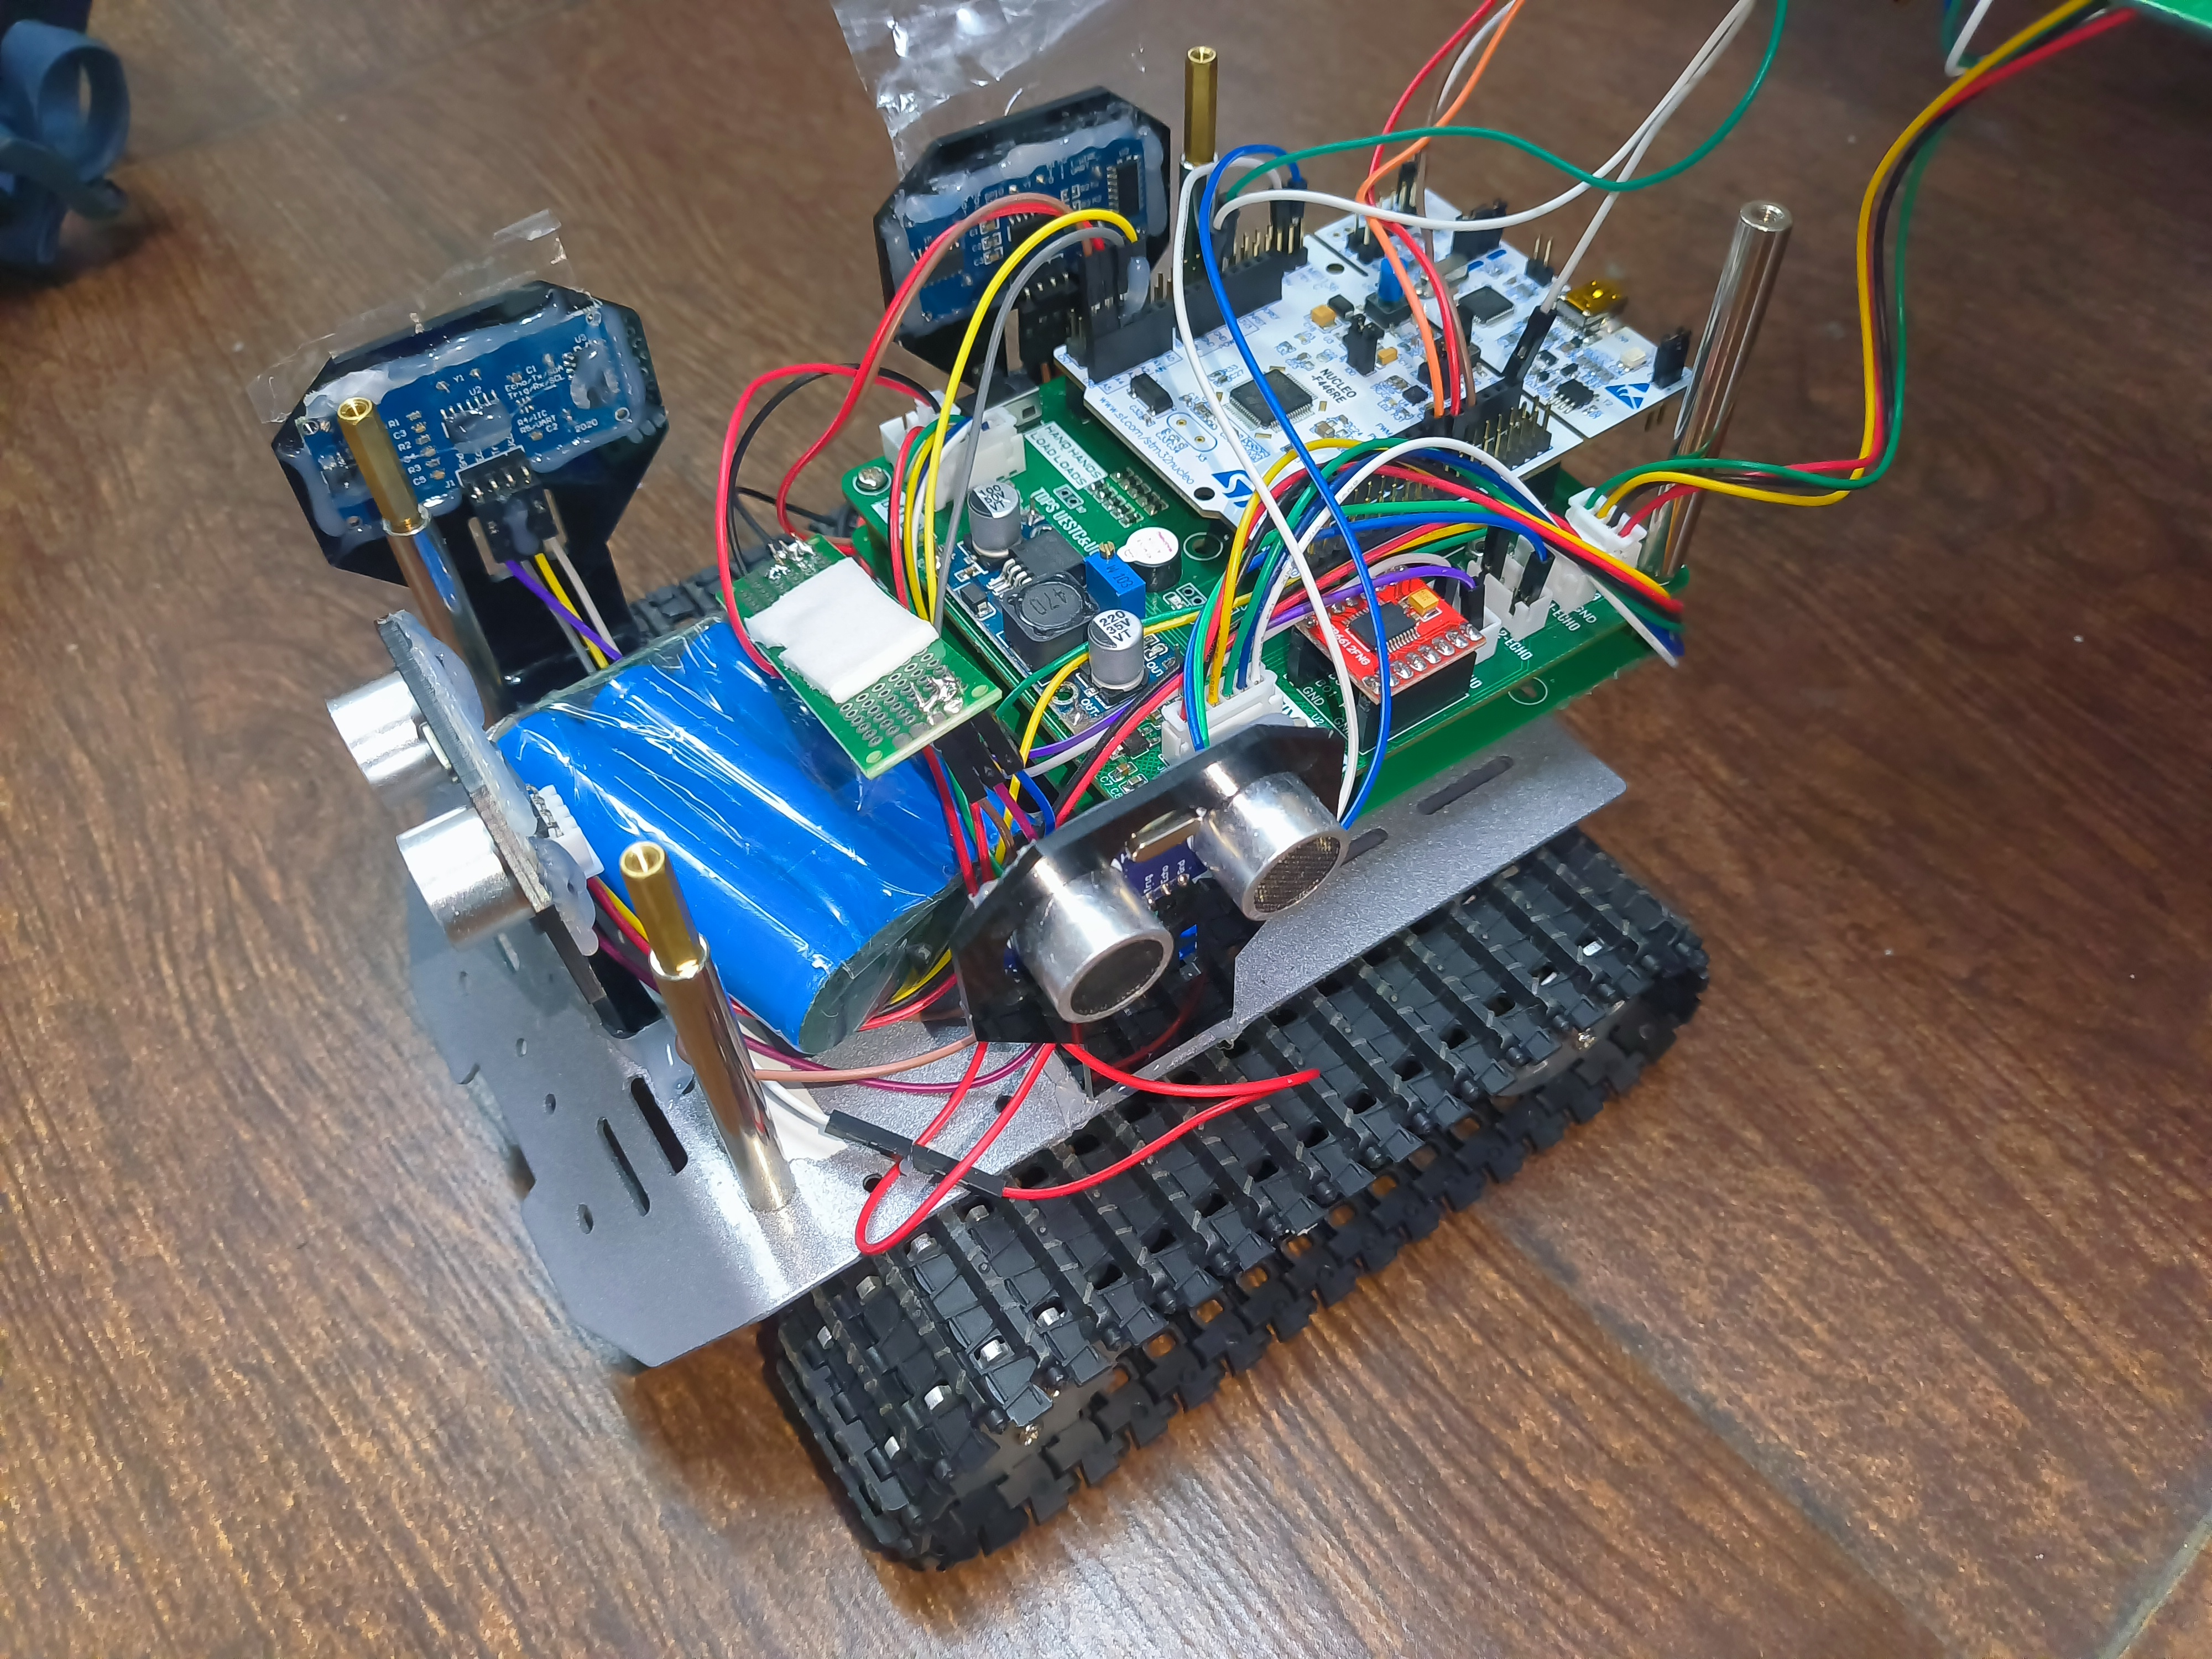
\includegraphics[width=0.7\textwidth]{pic/Hardware Design/Overall Image of The Rover.jpg}
\caption{Overall Image of The Rover}
\label{fig:Overall Image of The Rover}
\end{figure}
\begin{figure}[H]
\centering
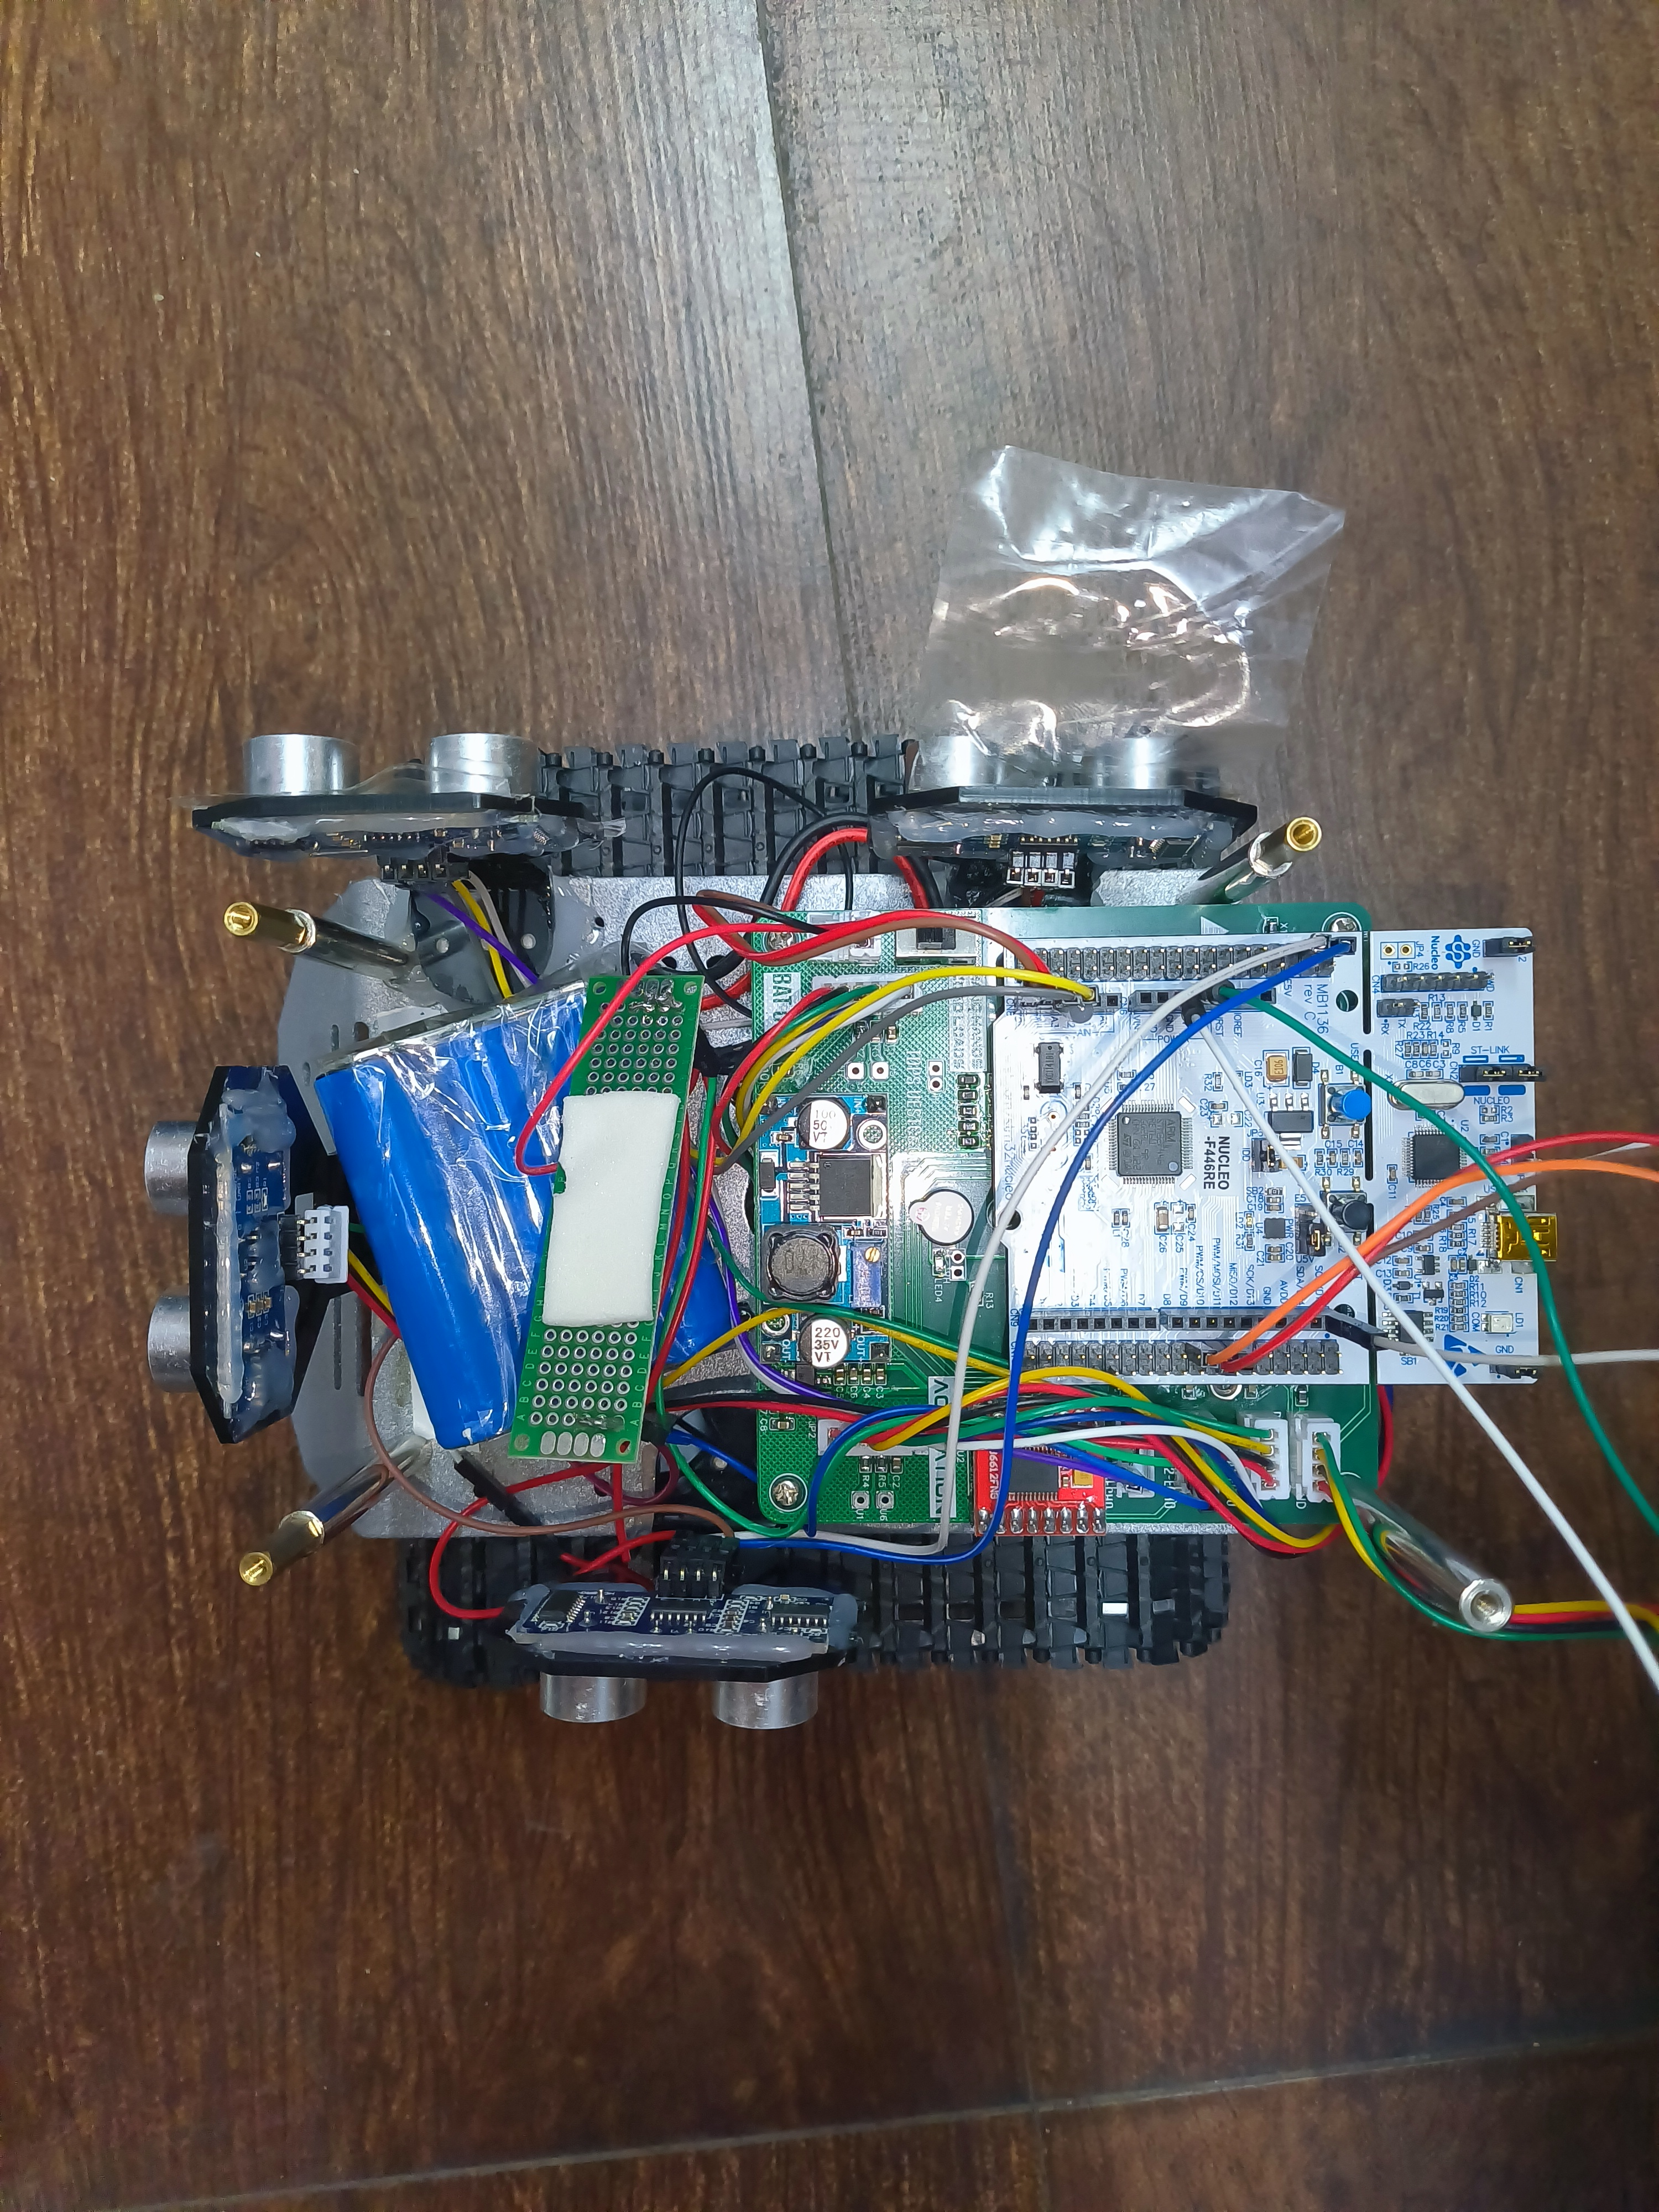
\includegraphics[width=0.6\textwidth]{pic/Hardware Design/Top View.jpg}
\caption{Top View}
\label{fig:Top View}
\end{figure}
\subsubsection*{Lower Layer}
\begin{figure}[H]
\centering
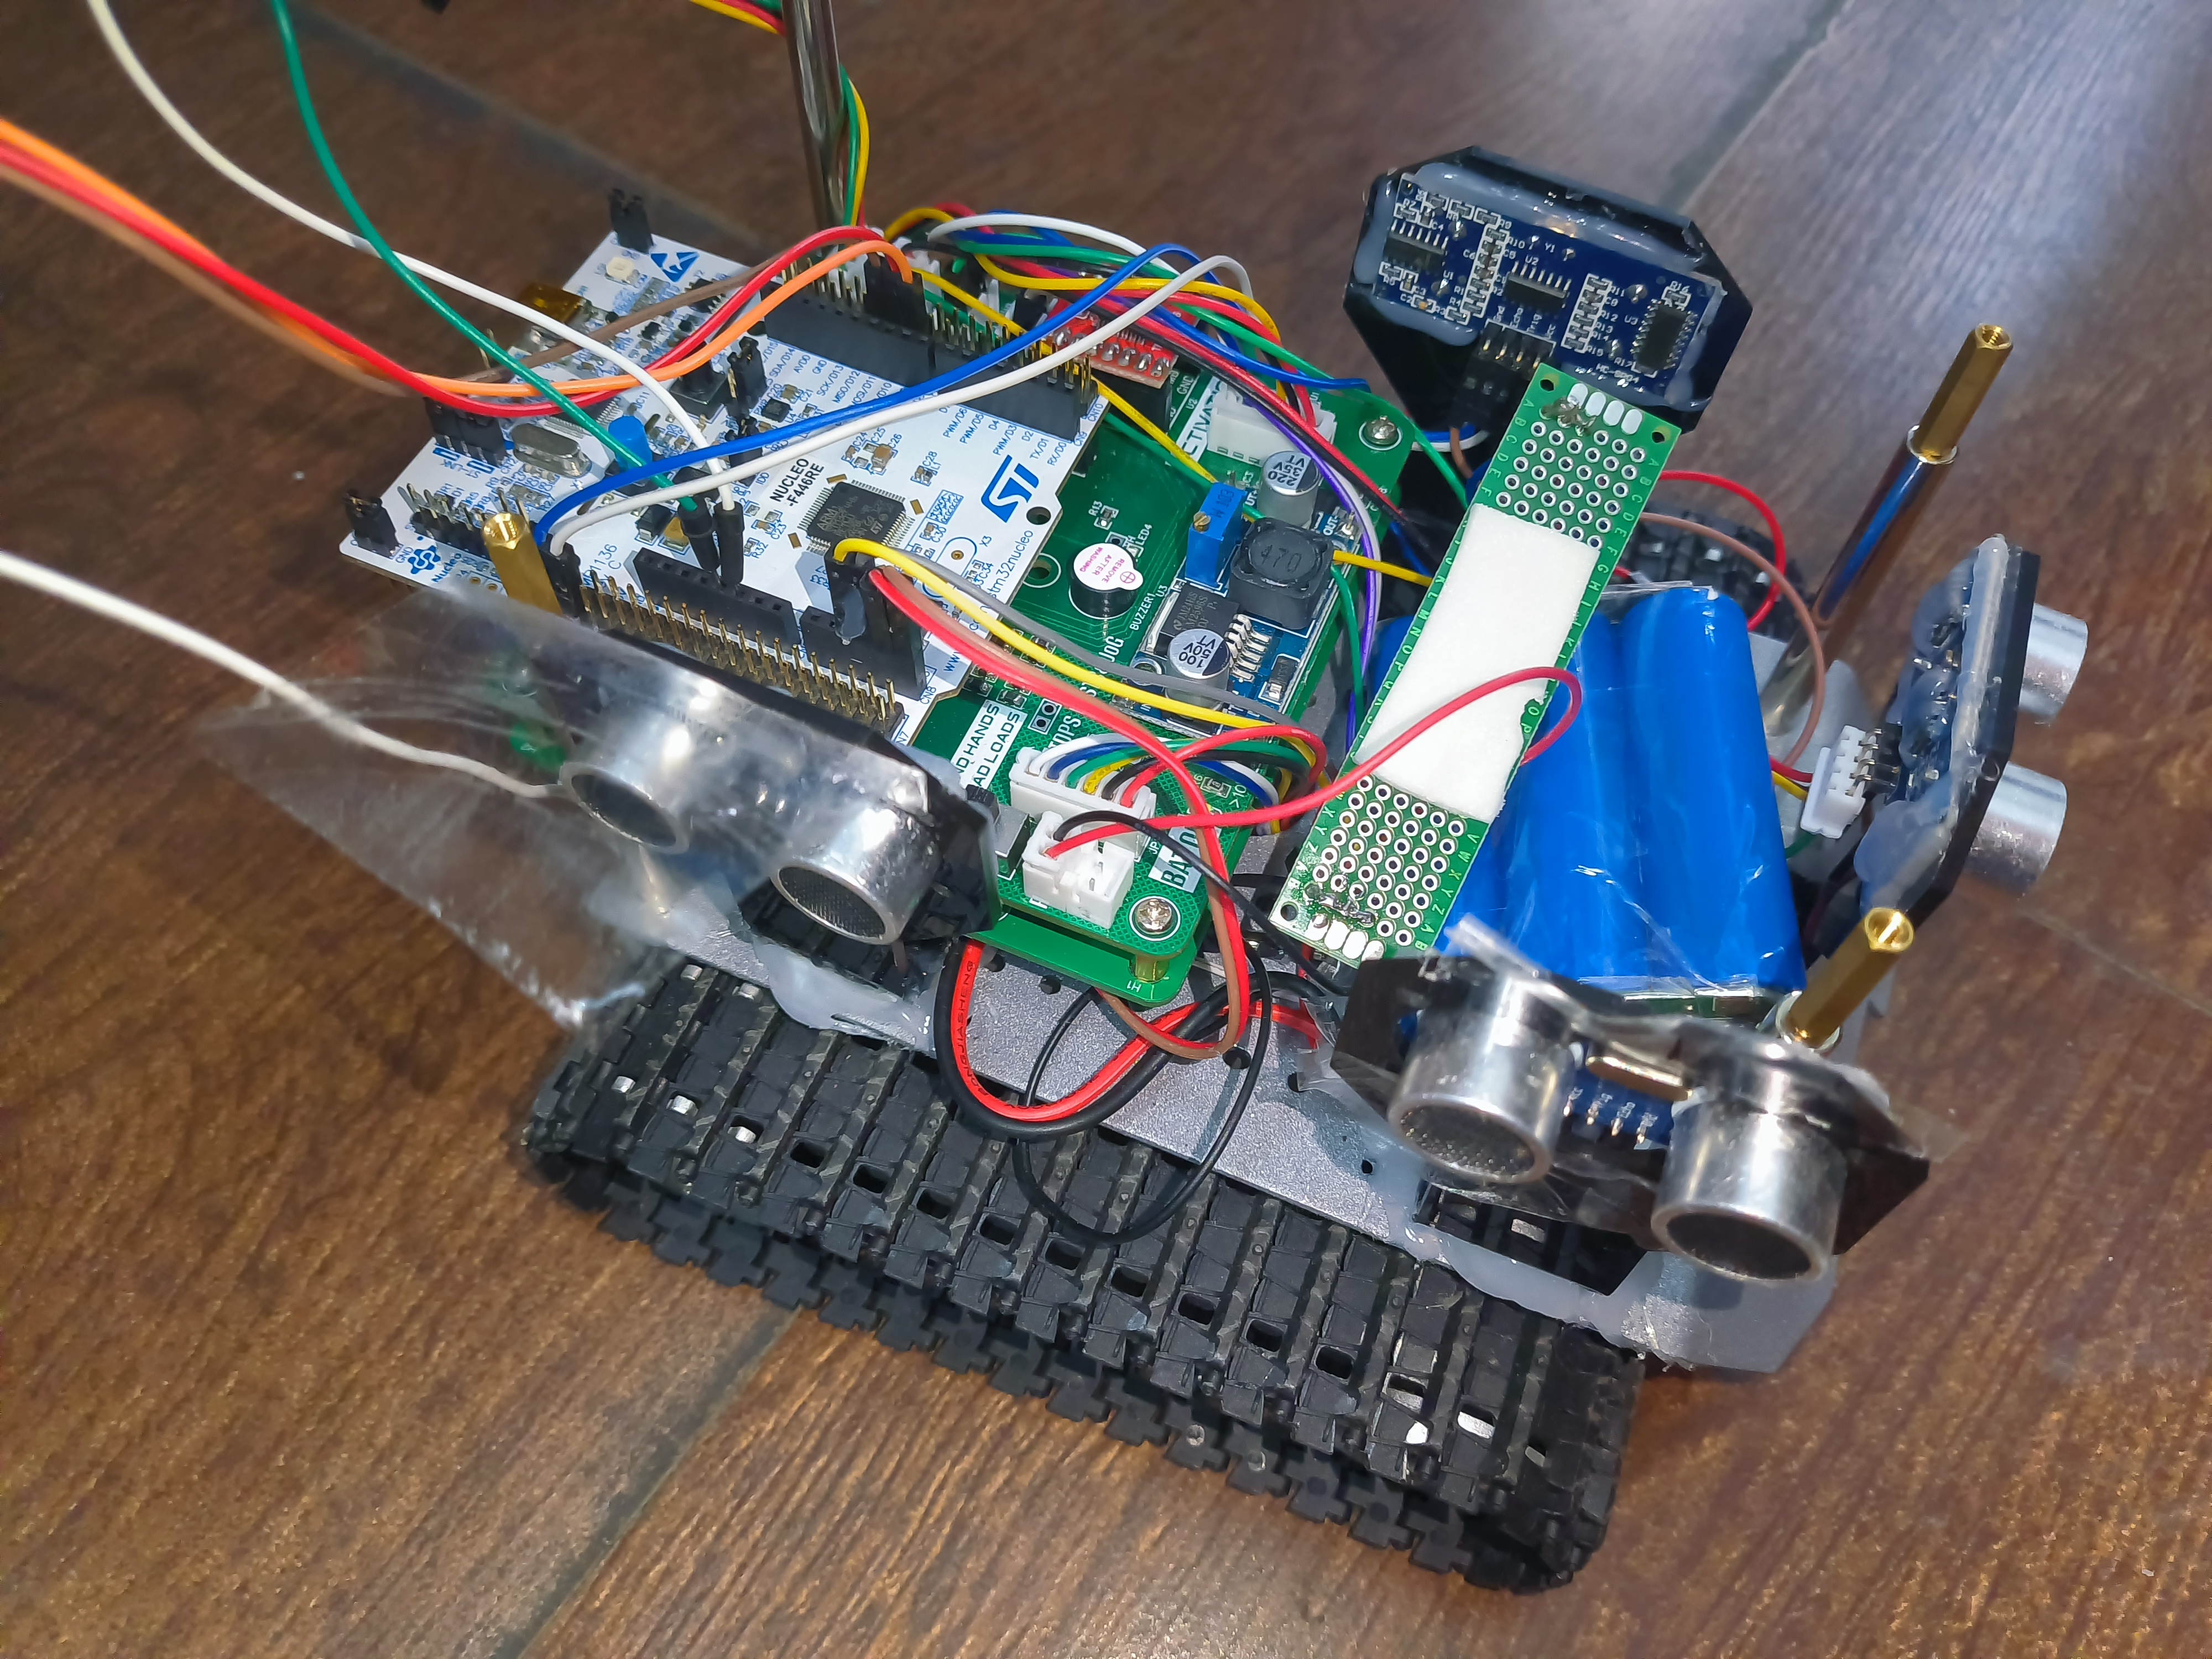
\includegraphics[width=0.5\textwidth]{pic/Hardware Design/Lower Layer.jpg}
\caption{Lower Layer}
\label{fig:Lower Layer}
\end{figure}

The lower layer mounts our self-designed and developed PCB and the STM32 on top of it. The battery is placed in front of the PCB. On the front side, on the left and right side, the ultrasonic modules needed are placed. The PCB and the STM32 are placed on the lower layer because the base board of the upper layer protects the electronic components from burning due to direct sunlight on a sunny day and from circuit damage due to rain on a rainy day. The ultrasonic module needs to match the height of the bottom of the railing in Patio 2 to complete the patrol, so it is also placed on the bottom layer.

    \subsubsection*{Upper Layer}
\begin{figure}[H]
  \centering
  \begin{minipage}[t]{0.48\textwidth}
    \centering
    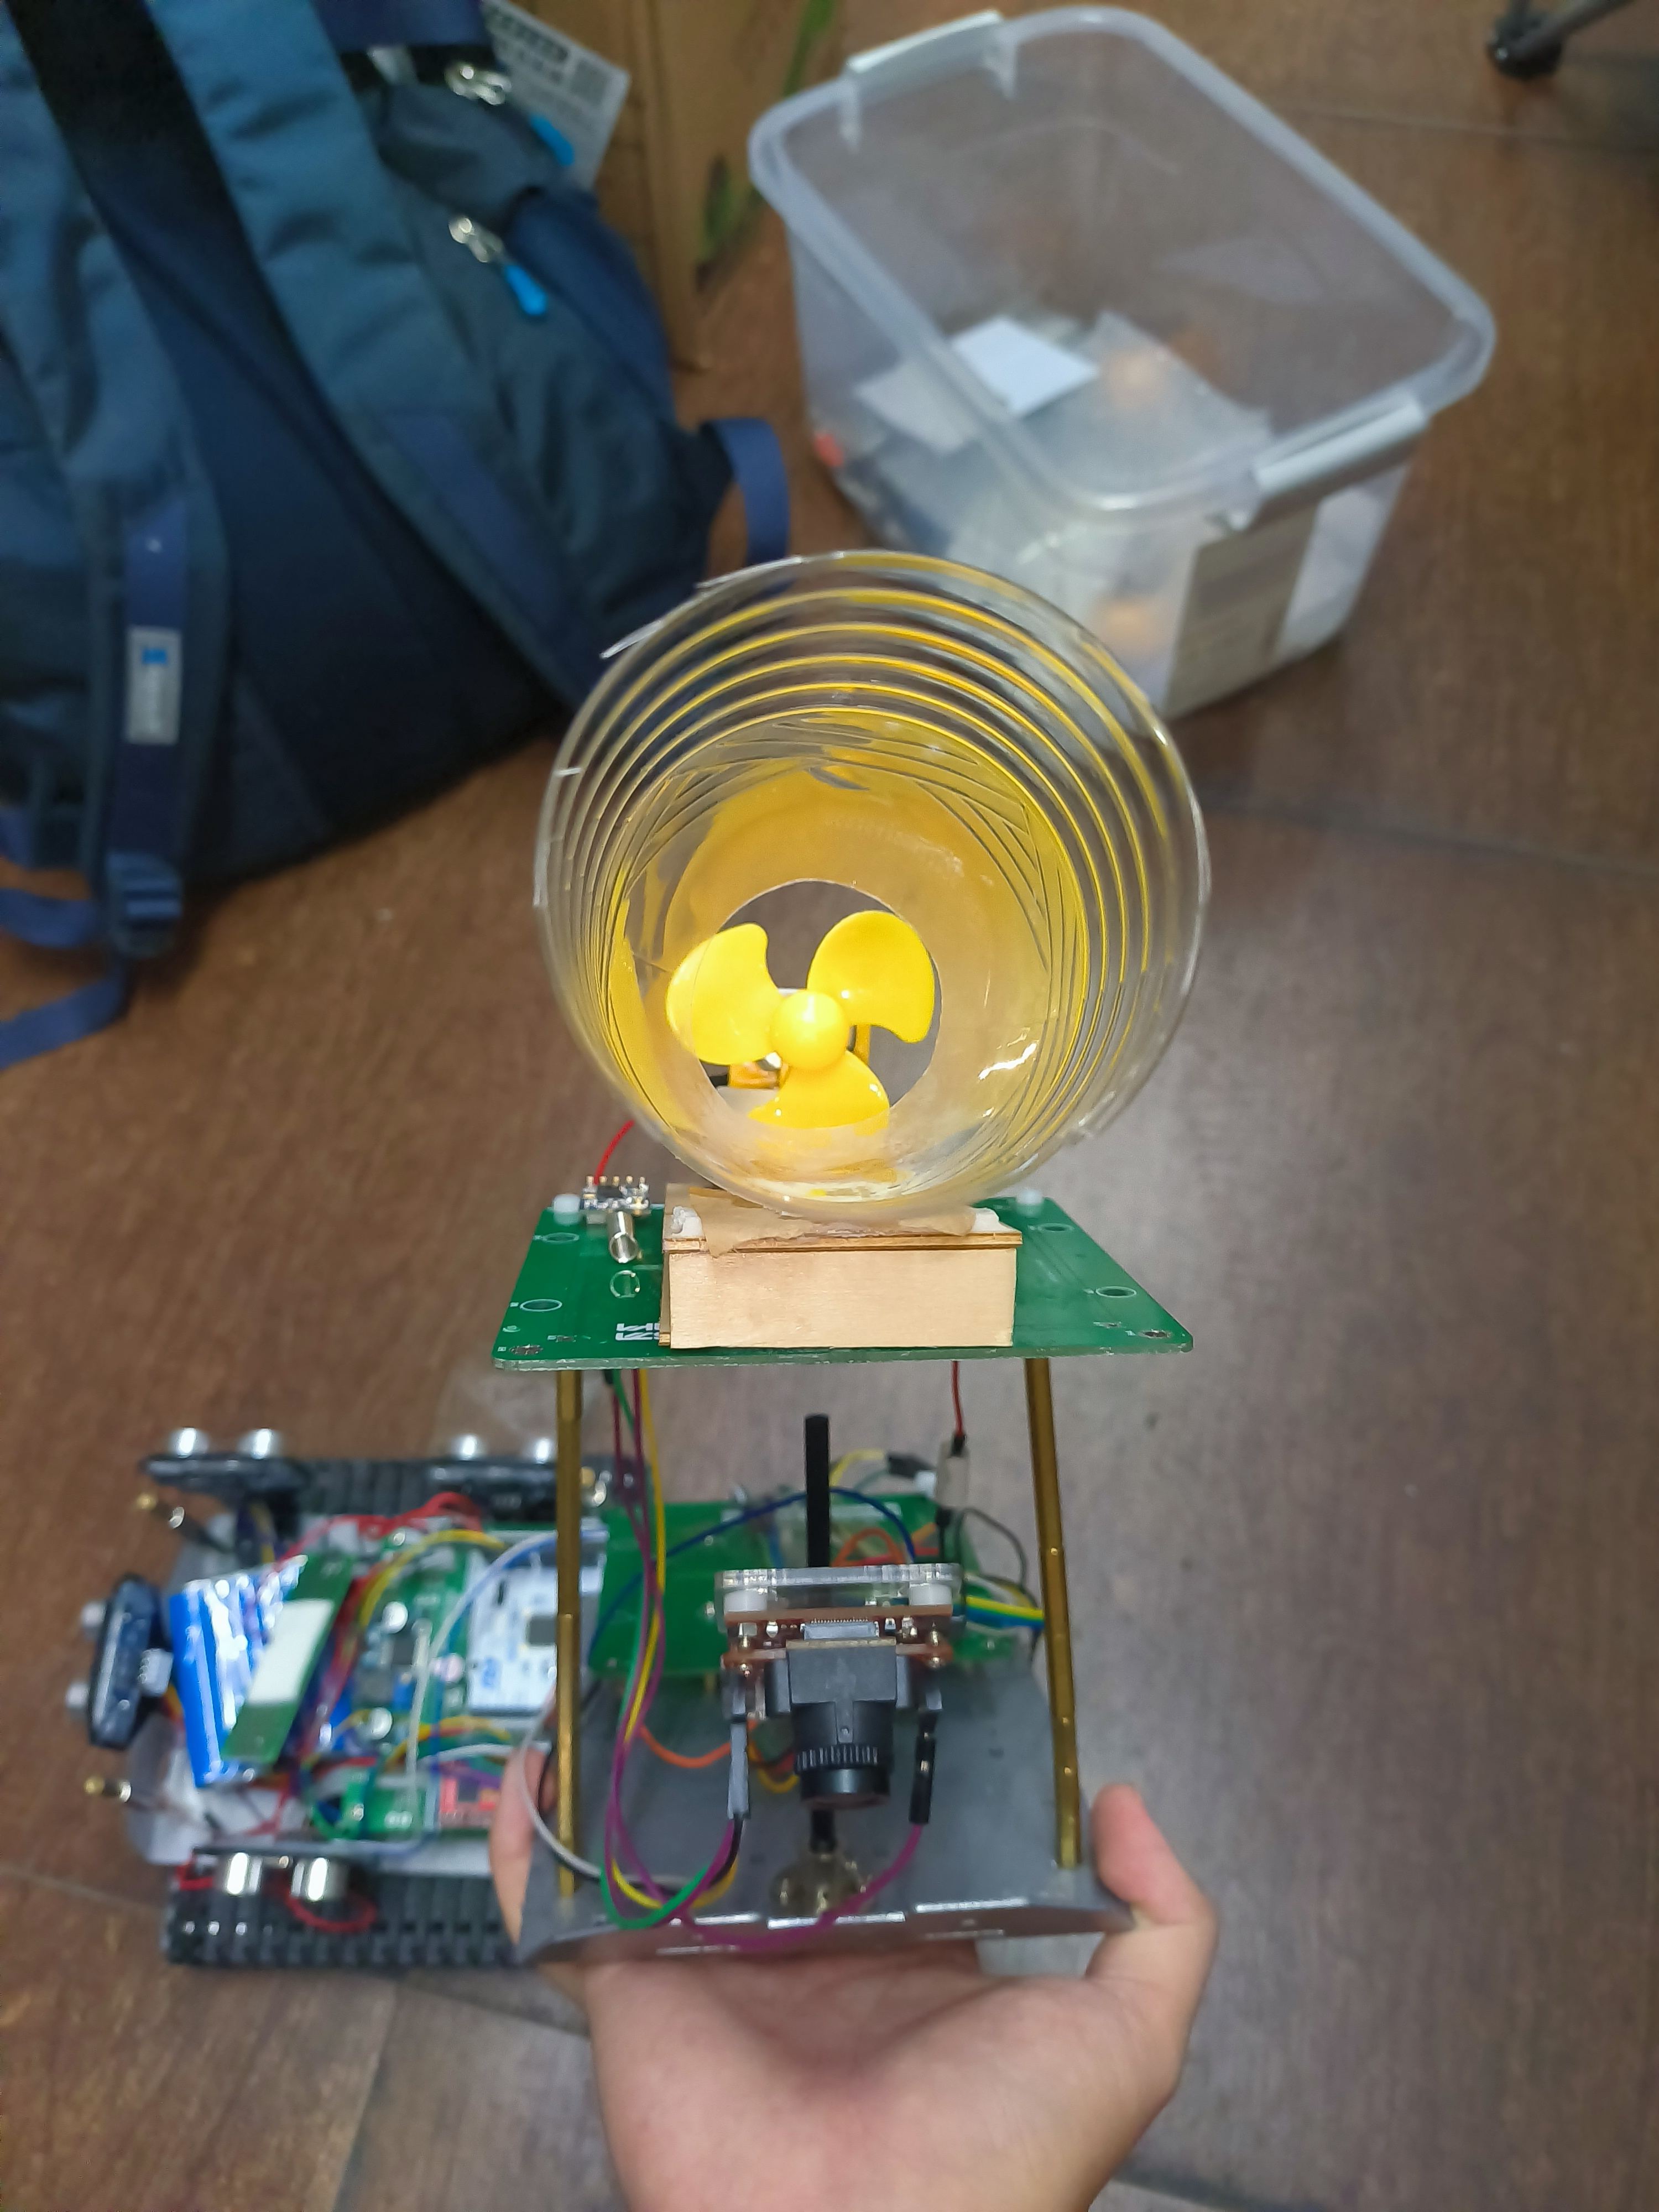
\includegraphics[width=\textwidth,height=0.38\textheight]{pic/Hardware Design/Upper Layer Front View.jpg}
    \subfigure{Upper Layer Front View}
    \label{fig:Upper Layer Front View}
  \end{minipage}\hfill
  \begin{minipage}[t]{0.48\textwidth}
    \centering
    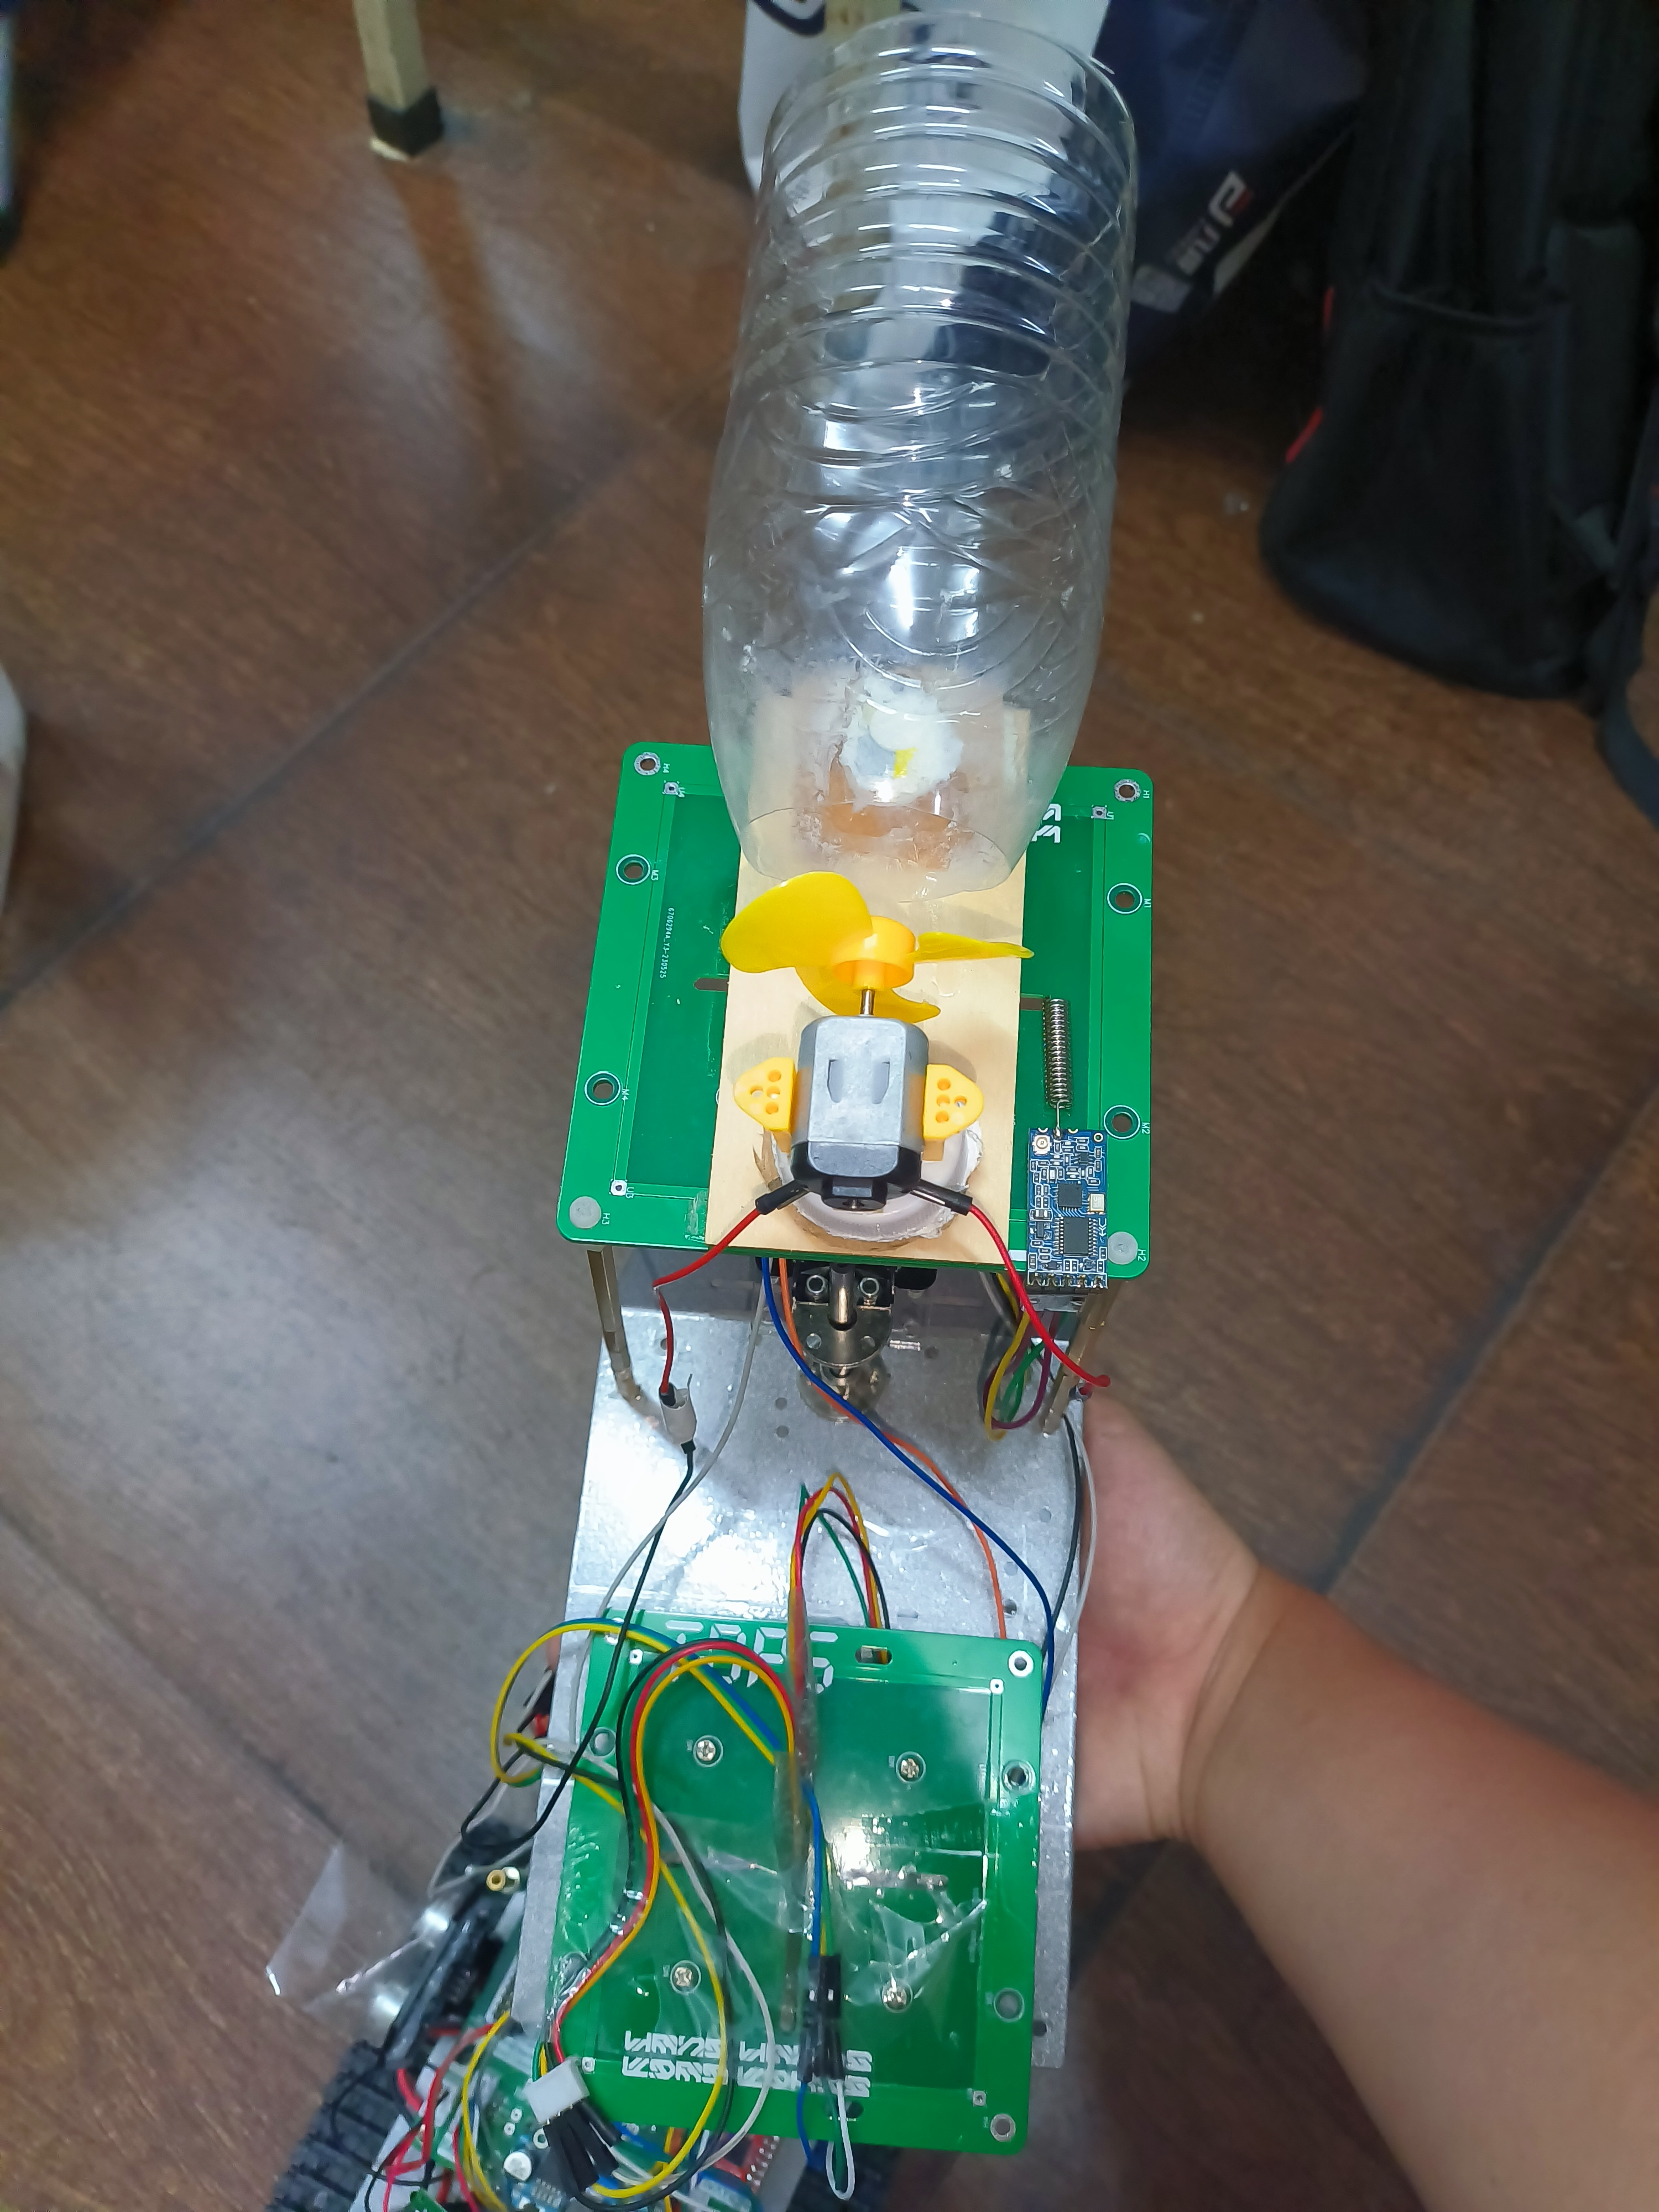
\includegraphics[width=\textwidth,height=0.38\textheight]{pic/Hardware Design/Upper Layer Back View.jpg}
    \subfigure{Upper Layer Back View}
    \label{fig:Upper Layer Back View}
  \end{minipage}
  \caption{Upper Layer}
  \label{fig:both_images}
\end{figure}








The picture here shows the upper layer, with the OpenMV and the table tennis release module. They are placed on the upper level because in Patio 1 the OpenMV needs to be at a certain height above the ground to achieve a better view and to simplify the optimisation of the patrol algorithm. Too low a height will result in worse viewing angles. In Patio 2 the arrow recognition part also needs the OpenMV to be at an appropriate height above the ground to match the arrow. The table tennis release module also needs to match the height of the bucket to ensure that the ball falls smoothly into the bucket. 

\subsection{Description of Some Components}
\subsubsection*{Steel Sheet}
Steel plate structures have high strength and are resistant to breakage or deformation, making them an ideal material for constructing the base plate. Furthermore, there are numerous manufacturers available for custom-made steel plates, allowing us to quickly obtain the desired steel plates at a lower cost. We simply need to provide the corresponding dimensions, and the manufacturer can promptly cut and deliver the plates to us.

\subsubsection*{Copper Column}
Copper columns were chosen as the material for connecting and securing the upper and lower layers. Its structural strength meets the requirements and it is corrosion-resistant, preventing rusting and satisfying the need for long-term outdoor testing. Additionally, during the vehicle's operation, the screws tightly engage with the copper columns, preventing excessive vibrations caused by inadequate fixation between the upper and lower layers, thereby greatly reducing the risk of damage to electronic components. Different lengths of copper columns were used in the actual construction process to accommodate various needs.
    
\subsubsection*{Tracked Drive System}
We adopted a tracked drive system instead of the traditional wheeled drive system because the tracked drive system offers several advantages that the wheeled system lacks. Firstly, traditional wheeled vehicles require four motors to control four wheels, which makes it more challenging to develop a drive system for a smart vehicle. In contrast, a tracked vehicle only requires two motors to control the main wheels of each track, significantly simplifying the drive system. Secondly, tracked vehicles perform better in off-road and climbing tasks, providing smoother travel on various ground surfaces.
    
\subsection{Analysis and Discussion}
In fact, during the entire vehicle assembly process, we encountered major challenges in the early stages, including the selection of the vehicle's drive system, the choice of base plate material, and the design of the vehicle's structure.

For the drive system, we ultimately chose a tracked system instead of the traditional wheeled system. The tracked system provided better off-road capabilities and maneuverability, while also simplifying the motor control system, reducing development time and cost.

We considered three materials for the base plate: carbon fiber, acrylic, and steel. Carbon fiber offers high strength and lightweight properties, but it has longer processing times, higher costs, and limited availability of processing plants, which made it less suitable for our project. Acrylic, on the other hand, has a favorable cost-performance ratio and numerous processing plants, but we had concerns about its structural strength. Ultimately, we chose steel as the base plate material because there are many processing plants specializing in steel cutting, allowing us to quickly obtain the desired base plate at a lower cost, effectively reducing development time and cost.

Copper was chosen as the material for the fixing pillars due to its availability in various lengths. Additionally, its corrosion resistance and non-rusting properties met the requirements for long-term outdoor testing of the vehicle.

Since each layer of the base plate was designed independently and then manufactured by processing plants, we had precise control over the dimensions of the steel base plate. This allowed us to meet the requirements of accommodating all electronic components while maintaining flexibility in design.
\begin{table}[h!]
  \begin{center}
    \caption{Comparison of Materials to be selected}
    \begin{tabularx}{\textwidth}{|X|X|X|X|}
      \hline      
      \textbf{Material} & \textbf{Density $g/{cm}^3$} & \textbf{Tensile Strength $Mpa$} & \textbf{Additional Characteristics}\\
      \hline
      carbon fiber & 1.5 & 3400 & Fatigue-resistant 
      
      Corrosion-resistant\\
      \hline
      acrylic & 1.2 & 50 & Cheap 
      
      Wear-resistant 
      
      Easy processing\\
      \hline
      Steel & 8 & 515 &  Corrosion-resistant 
      
      High hardness\\
      \hline
      Copper & 8.96 & 200-350 & Corrosion-resistance\\
      \hline
    \end{tabularx}
  \end{center}
\end{table}
\newpage
\section{Circuit Drive}\label{sec:CD}
\colorbox{yellow}{\textbf{Developer 1:} Zheng Jiashu 2614397L}

\colorbox{yellow}{\textbf{Developer 2:} Gao Tianji 2614386G}

\subsection{Motor Drive}
\subsubsection{Importance}
On the one hand, if the motor is directly controlled by a microcontroller unit (MCU) whose load capacity is often weak, the power output of the DigitalOut pin of the MCU is insufficient to drive the motor to work. Even if the voltage of 3.3V or 5V meets the requirements of the motor, the current intensity may be too small to successfully rotate the motor because the DC motor is usually a large current inductive load. In this case, the MCU may also be burned out due to continuous full load output. On the other hand, if the motor is directly powered by a power supply, the system cannot control the speed and direction of the motor. Therefore, the motor driver is a necessary component used to connect the motor, MCU, and power supply together and protect the circuit.

\subsubsection{TB6612FNG Module}
TB6612FNG as shown in Figure \ref{fig:mt1} is a high voltage driver IC for DC motor with output transistor in LD MOS structure with low ON-resistor \cite{zzs1}. One TB6612FNG driver chip can control two DC motors to do different actions at the same time. It can output 3.2A current at most in the voltage range of 2.5V to 13.5V, and features overheating self-breaking and feedback detection \cite{zzs1}. TB6612FNG can directly control the motor, set its control level through the input of the main control chip, and then it can drive the motor in forward and reverse rotation, with simple operation and excellent stability, which meets the large current driving requirements of DC motor. 

\begin{figure}[H]
  \centering
  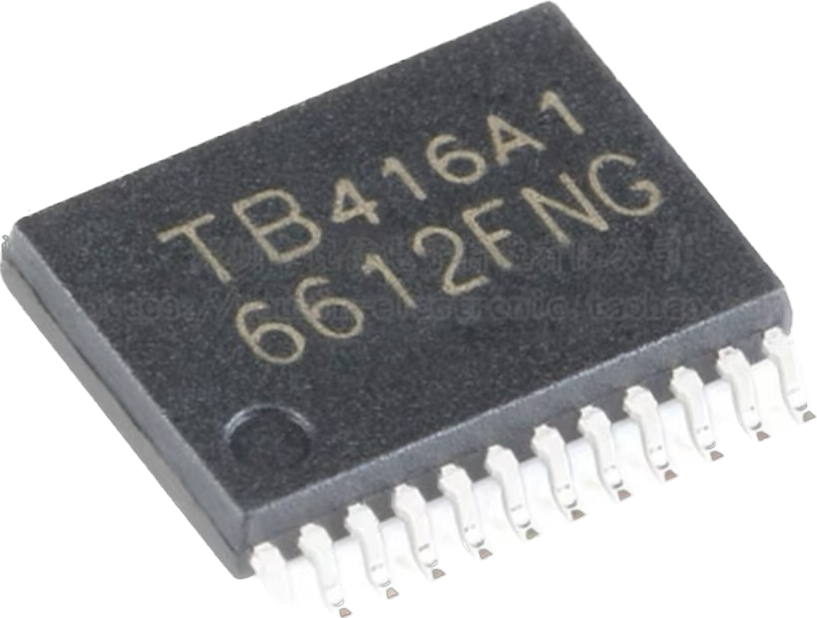
\includegraphics[width=0.35\textwidth]{pic/Motor Drive/1.png}
  \caption{TB6612FNG \cite{zzs1}}
  \label{fig:mt1}
\end{figure}

\subsubsection{Principle}
Figure \ref{fig:mt2} shows the inside structure of TB6612FNG. $V_{cc}$ provides power supply for control logic circuits. $V_m$ provides power supply for output to drive motors. The STYB detects the chip status to control the standby mode, based on the rule that a high-level (3.3V/5V) input will enable and a low-level input will put it into standby \cite{zzs1}. As for the control logic shown in Table \ref{tab:mt1} and the MOSFET-H bridge circuit shown in Figure \ref{fig:mt3}, they are the key to achieving the chip's function.

\begin{figure}[H]
  \centering
  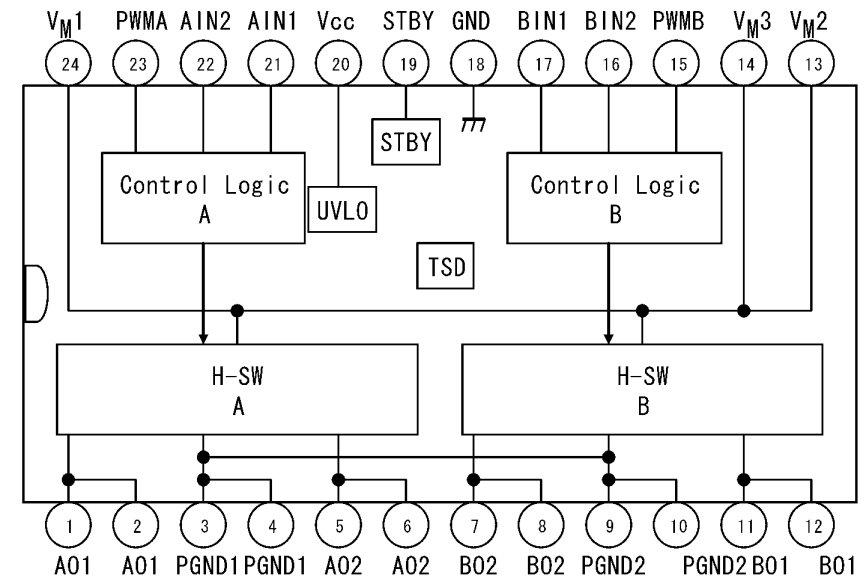
\includegraphics[width=0.6\textwidth]{pic/Motor Drive/2.png}
  \caption{TB6612FNG \cite{zzs1}}
  \label{fig:mt2}
\end{figure}

\begin{table}[H]
    \centering
    \begin{tabular}{|c|c|c|}
    \hline
        IN1 & IN2 & Conducted MOSFET \\ \hline
        1 & 0 & Q2 Q3 \\ \hline
        0 & 1 & Q1 Q4 \\ \hline
        1 & 1 & Q2 Q4 \\ \hline
        0 & 0 & None \\ \hline
    \end{tabular}
    \caption{The Control Logic} 
    \label{tab:mt1}
\end{table}

For example, if the input for IN1 is high-level signal and for IN2 is low-level signal, that is, 10, Q1, Q4 are on and Q2, Q3 are off as shown in Figure \ref{fig:mt3}(a). The current flows from Q1, from the positive terminal of the motor, through the negative terminal of the motor, and then out of Q4, completing a circuit in which the motor will rotate in a certain direction.

\begin{figure}[H]
  \centering
  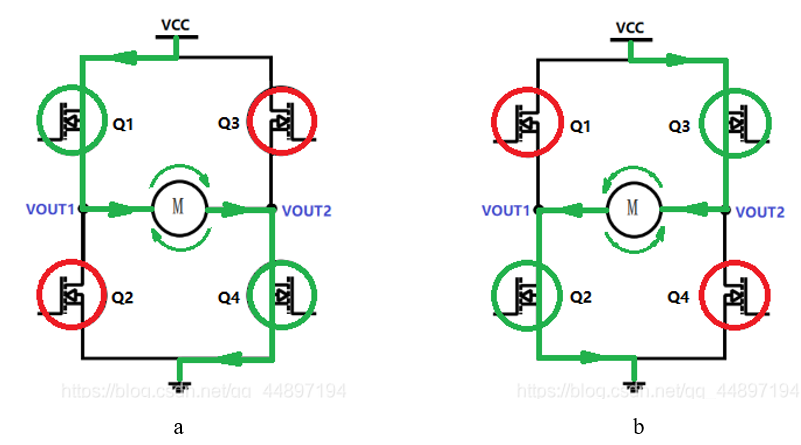
\includegraphics[width=0.6\textwidth]{pic/Motor Drive/3.png}
  \caption{H Bridge Circuit}
  \label{fig:mt3}
\end{figure}

In Figure \ref{fig:mt3}(b), if the input for IN1 is low-level signal and for IN2 is high-level signal, that is, 01, Q1, Q4 are off and Q2, Q3 are on. The current flows from Q3, from the positive terminal of the motor, through the negative terminal of the motor, and then out of Q2, completing a circuit in which the motor will rotate in an inverse direction.

\subsubsection{Circuit Design}
Circuit shown in Figure \ref{fig:mt4} was the design of our motor drive which use a TB6612FNG. The same interface except GND of the chip is combined into 1 pin in this circuit. Meanwhile for $V_{cc}$ and $V_m$, filtering capacitors are connected between the pin of the chip and the pin of the motor drive to prevent noise interference. 

\begin{figure}[H]
  \centering
  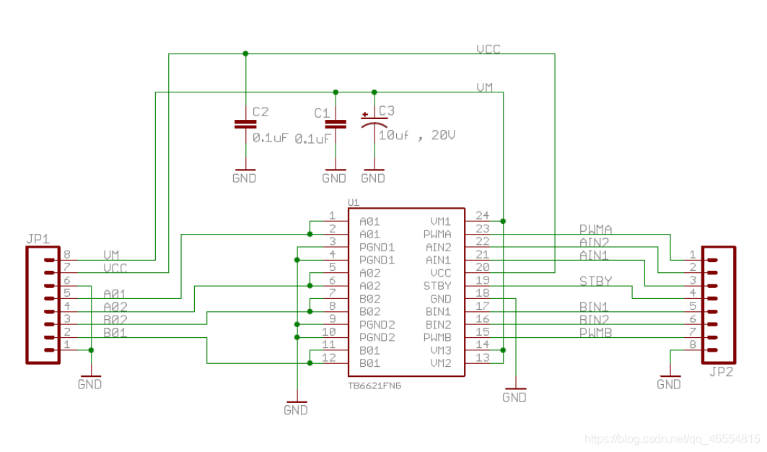
\includegraphics[width=1\textwidth]{pic/Motor Drive/4.png}
  \caption{The Design of Our Motor Drive Based on TB6612FNG}
  \label{fig:mt4}
\end{figure}

\subsubsection{Application}

According to our design in Figure \ref{fig:mt4}, there are 14 different pins and the usage of each pin of the motor drive is shown in Table \ref{tab:mt2}.

\begin{table}[H]
    \centering
    \begin{tabular}{|c|c|c|}
    \hline
        PIN & Function & Connection \\ \hline
        VM & Motor drive voltage & 2.5 to 13.5V supply \\ \hline
        VCC & Chip drive voltage & 3.3V or 5V supply \\ \hline
        STBY & Activate the chip & 3.3V or 5V supply \\ \hline
        PWMA & PWM control for motor A & MCU \\ \hline
        PWMB & PWM control for motor B & MCU \\ \hline
        AIN1, AIN2 & Logic input for motor A & MCU \\ \hline
        BIN1, BIN2 & Logic input for motor B & MCU \\ \hline
        AO1, AO2 & Output of motor A & Motor A \\ \hline
        BO1, BO2 & Output of motor B & Motor B \\ \hline
        GND & 0V reference potential level & Common ground with MCU \\ \hline
    \end{tabular}
    \caption{The Usage of Each Pin}
    \label{tab:mt2}
\end{table}
\newpage
According to the control logic and the design of the circuit, the truth table to this motor drive can be summarized as shown in Table \ref{tab:mt3}. It is obvious that, two input signals, IN1 and IN2, can choose one of three modes such as CW, CCW, and Stop mode, which is the most important reference for us to write codes for controlling the rover to turn right, turn left or stop.

\begin{table}[H]
    \centering
    \begin{tabular}{|c|c|c|c|c|c|c|}
    \hline
         \multicolumn{4}{|c|}{INPUT} & \multicolumn{3}{|c|}{OUTPUT} \\ \hline
        IN1 & IN2 & PWM & STBY & OUT1 & OUT2 & MODE \\ \hline
        H & H & H/L & H & L & L & Short brake \\ \hline
        L & H & H & H & L & H & \textcolor{red}{CCW}\\ \hline
        L & H & L & H & L & L & Short brake \\ \hline
        H & L & H & H & H & L & \textcolor{red}{CW} \\ \hline
        H & L & L & H & L & L & Short brake \\ \hline
        L & L & H & H & \multicolumn{2}{|c|}{High Impedance} & \textcolor{red}{Stop} \\ \hline
        H/L & H/L & H/L & L & \multicolumn{2}{|c|}{High Impedance}& Standby \\ \hline
    \end{tabular}
    \caption{Truth table for motor drive \cite{zzs1}}
    \label{tab:mt3}
\end{table}


\subsection{Master Control Unit}
\subsubsection{Selection Criteria}
Based on the analysis of the various modules in the appeal, we have summarised some of the requirements for the main MCU:
 \begin{enumerate}

\item  There is a sufficient number of pins to meet the requirement to integrate and connect all components such as motor drivers, openmv, HC-SR04 etc.
\item The functions of ports of the master MCU needs to be sufficient for the communication between the modules to control them, e.g. UART, IIC, GPIO, etc.
\item The master MCU should have the ability to supply power to external components (3.3V and 5V) in order to facilitate the proper operation of the table tennis ball release module and IMU.
\end{enumerate}



\subsubsection{STM32}
STM32F446RE (STM32) as shown in Figure \ref{fig:mt5} was chosen as our master MCU to run the controlling code to control or communicate with all modules mentioned above. The STM32 board provides an affordable and flexible way for us to try out new concepts and build prototypes by choosing from the various combinations of performance and power consumption features, provided by the STM32 microcontroller.

\begin{figure}[H]
  \centering
  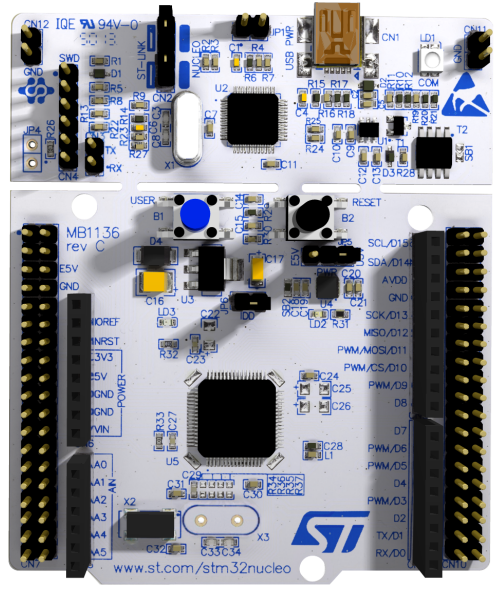
\includegraphics[width=0.35\textwidth]{pic/Motor Drive/15.png}
  \caption{STM32 Nucleo-64 board \cite{zzs3}}
  \label{fig:mt5}
\end{figure}

The STM32 are based on the high-performance Arm Cortex-M4 32-bit RISC core operating at a frequency of up to 180 MHz \cite{zzs3}. The Cortex-M4 core features a floating point unit single precision supporting all Arm single-precision data-processing instructions and data types \cite{zzs3}. It also implements a full set of DSP instructions and a memory protection unit that enhances application security \cite{zzs3}. The STM32 board incorporate high-speed embedded memories (Flash memory up to 512 Kbytes, up to 128 Kbytes of SRAM), up to 4 Kbytes of backup SRAM, and an extensive range of enhanced I/Os and peripherals connected to two APB buses, two AHB buses and a 32-bit multi-AHB bus matrix \cite{zzs3}. All devices offer three 12-bit ADCs, two DACs, a low-power RTC, twelve general-purpose 16-bit timers including two PWM timers for motor control, two general-purpose 32-bit timers \cite{zzs3}.

\begin{figure}[H]
  \centering
  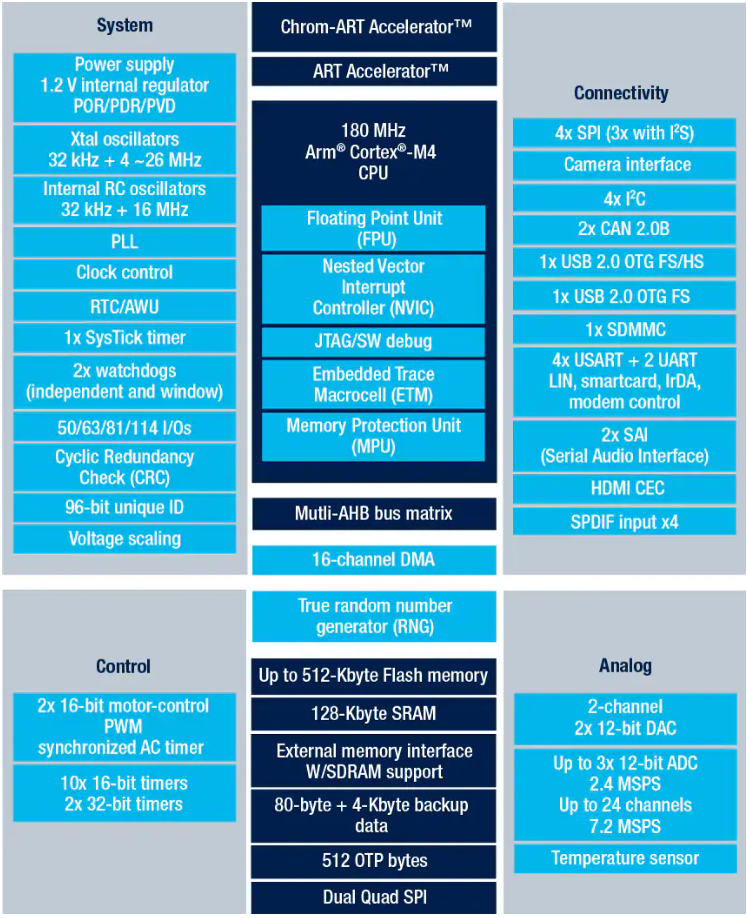
\includegraphics[width=0.45\textwidth]{pic/Motor Drive/16.png}
  \caption{Functions of STM32}
  \label{fig:mt6}
\end{figure}

Therefore, as shown in Figure \ref{fig:mt6}, STM32 provides sufficient ports to connect with. Eight General-Purpose Input/Output (GPIO) ports are allocated to the motors. Two I2C ports are used to receive the data from MPU-6050. One of the Universal Asynchronous Receiver/Transmitter (UART) ports to communicate with the visual module, receiving update from and sending commands to OpenMV. Besides, the GPIO ports could also be used to connect and control peripherals such as the HC-SR04.

\subsection{Signal Lines}
\begin{figure}[H]
  \centering
  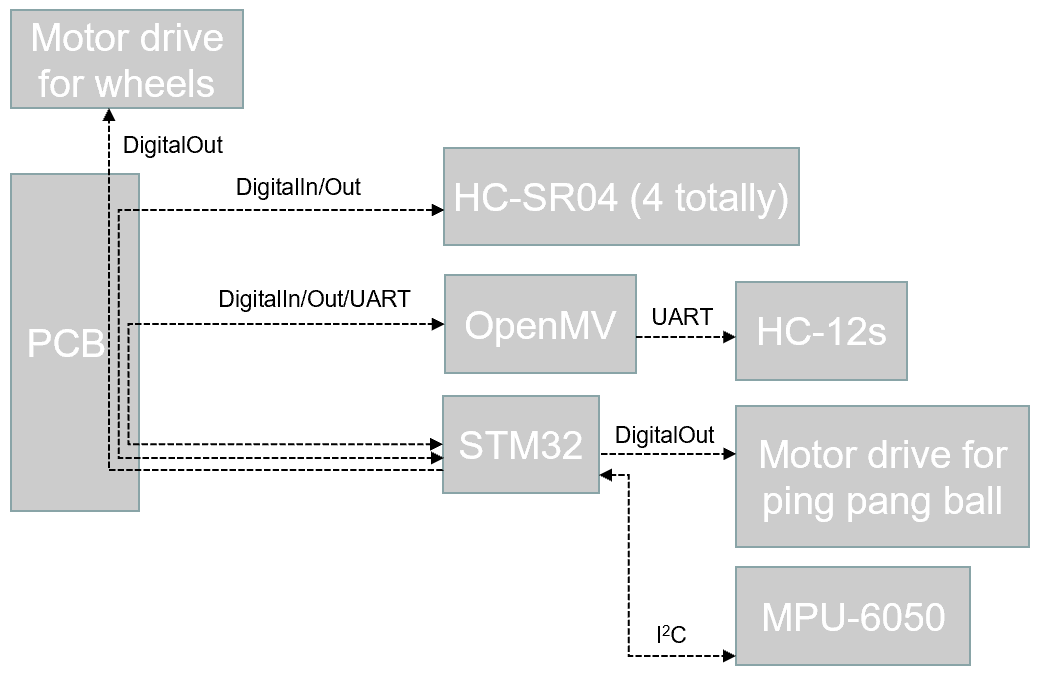
\includegraphics[width=0.8\textwidth]{pic/Motor Drive/17.png}
  \caption{Total signal path of our rover}
  \label{fig:mt7}
\end{figure}

As shown in Figure \ref{fig:mt7}, the communication between STM32 and OpenMV uses DigitalOut/In and UART methods which will be introduced later through the PCB. The communication between STM32 and HC-SR just uses DigitalOut/In through the PCB. Wheel motors are controlled by STM32 using DigitalOut method through PCB as well. HC-12 would receive the time information directly from OpenMV via UART transmission protocol. STM32 directly communicates with MPU-6050 via I2C transmission protocol and controls fan’s motor using DigitalOut method. The reason why signal lines for HC-12, motor of the fan and MPU-6050 do not go through the PCB is that wires connected to these components have to extend to their special location instead of being fixed in PCB which will be discussed by Si Yuan. In brief, the ping pong ball release device needs to be wired to the top layer of the rover in order to accommodate the height of the basket, while the HC-12 also needs to be mounted on the top layer in order for the signal to be transmitted smoothly outwards by the antenna. As for the MPU-6050, it needs to be installed on the most stable part of the rover - the chassis - to reduce the impact of vibration on the accuracy of the angle measurement.

\newpage
\subsection{Power Supply Distribution}
Figure \ref{fig:mt8} shows the power distribution for the whole rover.

\begin{figure}[H]
  \centering
  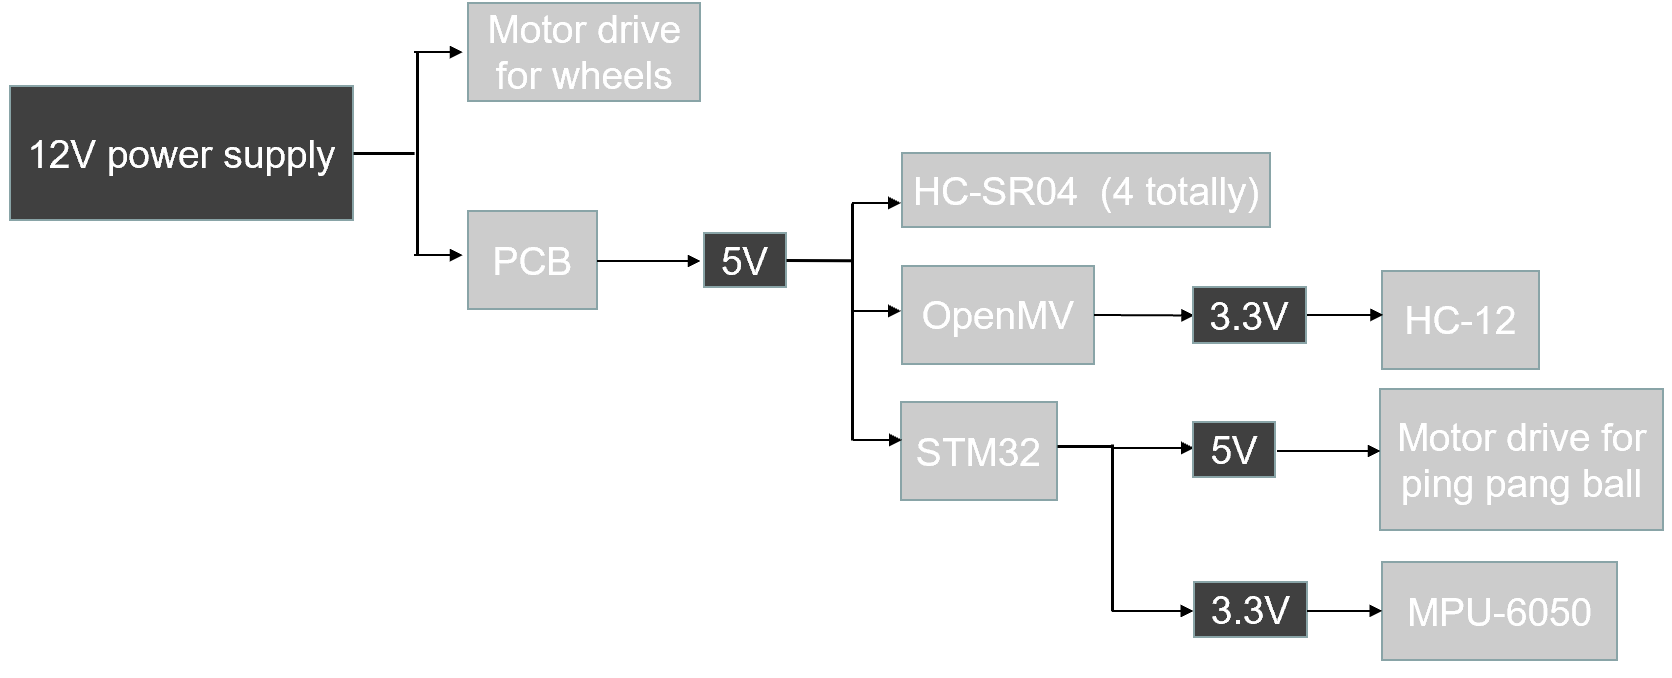
\includegraphics[width=1\textwidth]{pic/Motor Drive/18.png}
  \caption{Total power distribution of our rover}
  \label{fig:mt8}
\end{figure}

\subsubsection{12V Power Supply}
For powering the entire rover, the 12V LiPo battery as shown in Figure \ref{fig:mt9} is the best choice. The reasons for this are twofold. Firstly, 12V LiPo batteries which have the advantages of being offset in price and easy access to purchase are widely used to power trolley motors. Secondly, the motor that drives the rover to move needs a large enough voltage input to ensure dynamics, and meanwhile, a large voltage power supply can simply be stepped down to power other low power components, providing sufficient space for the design of other modules.

\begin{figure}[H]
  \centering
  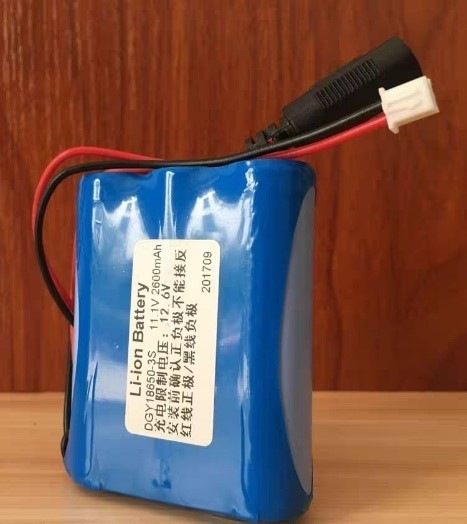
\includegraphics[width=0.5\textwidth]{pic/Motor Drive/19.jpg}
  \caption{Power supply for our rover}
  \label{fig:mt9}
\end{figure}

\subsubsection{5V After Bucking}
Obviously, 12V power supply is too high to power other modules, which means bucking is eaasential in PCB. There are two problems for this procedure, including the voltage magnitude after step-down and the design of step-down circuit.

By inveastugating the user manual of STM32 as shown in Figure \ref{fig:mt10} , it can be found that only when it is powered by about 5V input, there is no limitations. Forturnately, instruntions for components used in other modules such as OpenMV and HC-SR04 also adaptes 5V supply.

\begin{figure}[H]
  \centering
  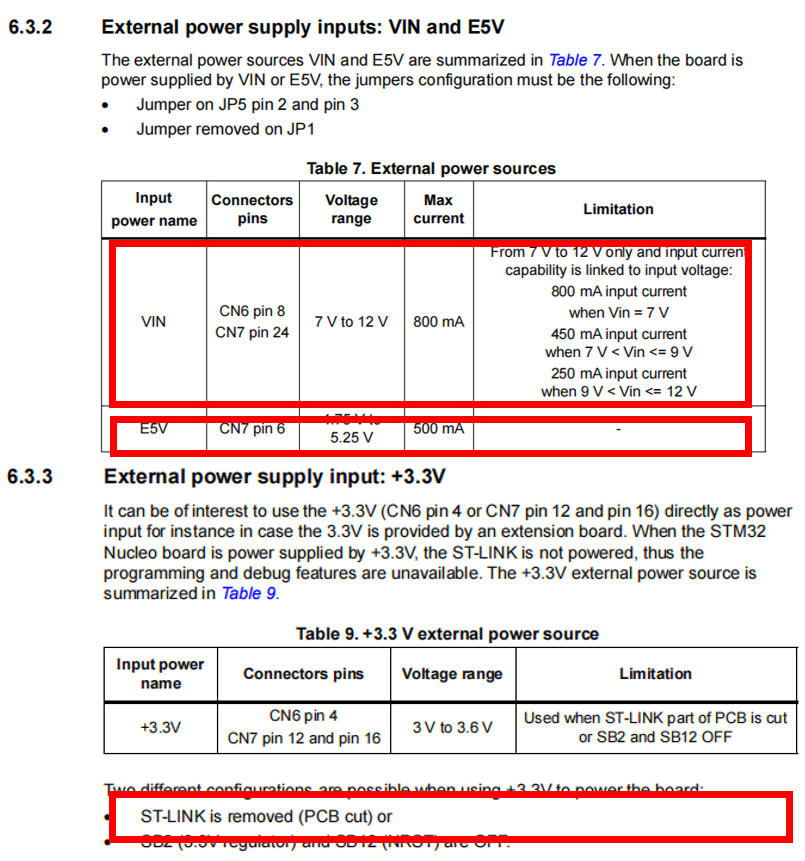
\includegraphics[width=0.9\textwidth]{pic/Motor Drive/20.png}
  \caption{Information about power supply input of STM32 \cite{zzs3}}
  \label{fig:mt10}
\end{figure}

There is the design for the step-down circuit in PCB shown in figure \ref{fig:mt11} which uses a three-band linear regulator L7805CV as shown in Figure \ref{fig:mt12}. The L7805CV is used to form a regulated power supply with very few peripheral components, and the chip has internal protection circuits for overcurrent, overheating and adjustment tubes, making it reliable, easy to use and inexpensive.

\begin{figure}[H]
  \centering
  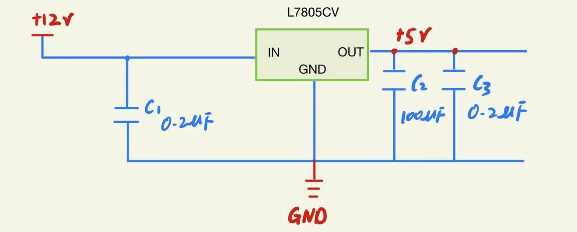
\includegraphics[width=0.9\textwidth]{pic/Motor Drive/21.png}
  \caption{DC buck circuit}
  \label{fig:mt11}
\end{figure}

\begin{figure}[H]
  \centering
  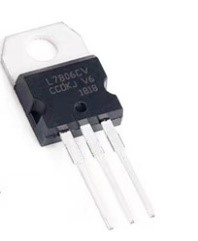
\includegraphics[width=0.3\textwidth]{pic/Motor Drive/22.jpg}
  \caption{L7805CV}
  \label{fig:mt12}
\end{figure}

The role of capacitors in the circuit shown in Figure \ref{fig:mt11} is as follows:

A bypass capacitor is connected in parallel to the input of the power supply: the bypass capacitor is an energy storage device that provides energy to the local devices, it homogenises the output of the regulator and reduces the load demand. The bypass capacitor is capable of being charged and discharged to the device. The bypass capacitor uses the interference in the input signal as a filter, and to minimise the impedance, it is important to be as close as possible to the supply power pin and ground pin of the load device, which can be a good protection against ground potential raising and noise caused by excessive input values. The input capacitor also protects the chip by preventing excessive voltage backflow at the output from burning the chip when power is lost.

The output of the power supply is connected in parallel with a decoupling capacitor: if the capacitance of the load in the circuit is relatively large, the power supply has to charge the capacitor to complete the signal jump. When the rising edge is steeper, the power supply current is higher and the inductors in the circuit (especially on the various chip pins) bounce back. This current is therefore effectively a noise and can affect the normal operation of the front stage. The decoupling capacitor takes this interference from the output signal as a filtering object to prevent the interfering signal from returning to the power supply to smooth out the voltage glitch, filter out high frequency noise and maintain a response time for the power supply after a power failure.

\subsubsection{Power Supply from STM32 and OpenMV}
The OpenMV can output a continuous 3.3V supply while the STM32 can output a continuous 3.3V or 5V supply. As already discussed in the signal lines, the signals are transmitted directly by wire from the OpenMV or STM32 to the HC-12, the motor drive of the ping pong ball release and the MPU-6050, so for convenience the power supply for these devices is also provided directly by the STM32 and OpenMV. In order to ensure that the fan has enough wind to suck in and blow out the ping pong balls, the motor has to drive the fan blades with enough wind to rotate them. Through the experiments mentioned in the notebook, a 5V supply was found to be a better option. Moreover, by investigating the HC-12 and MPU-6050 instructions, 3.3V was fortunately found to be just the appropriate supply voltage for them \cite{zzs2}.
    

    
\newpage
\section{PCB (Printed Circuit Board)}\label{sec:PCB}
\colorbox{yellow}{\textbf{Developer:} Liang Hengrui 2614017L}

PCB – the printed circuit board, is a system board that provide electrical connection and mechanical support for all elements assembled on it [1]. PCB is widely used in various kind of electronic devices to reduce volume and cost, provide stabler interconnection and higher performance and eventually increase the reliability of the product. In our smart vehicle project, a PCB board was designed, fabricated and applied to carry functional modules like STM-32, motor driver and power supply module. All the modules that are assembled on the PCB are listed in Table \ref{table:pcb1}
	\begin{table*}[!h]
	\centering
		\begin{tabular}{|c|c|c|}
		\hline
 \textbf{MODULE NAMES} &\textbf{FUNCTION} &\textbf{CONNECTION TO PCB} \\
  \hline
 \textbf{STM32} &Centre processor &Direct plug in  \\
 \hline
 \textbf{OPENMV} &Visual sensor  &Wire connection \\
 \hline
 \textbf{MOTOE DRIVER} & Drive fan and wheels & Direct plug in \& wire connection \\
 \hline
\textbf{POWER} & DC power supply & Direct soldering \& wire connection\\
\hline
\textbf{ULTROSONIC} & Sensor  & Wire connection\\
\hline
\textbf{BLUETOOTH} & Message transmission & Wire connection\\
\hline
\end{tabular}
\caption{The modules information that assembled on the PCB}
\label{table:pcb1}
	\end{table*}
	
\noindent
Meanwhile, the PCB also provides stable and simplified electrical connection between all functional modules. It prevented the massive use of connecting wires, improved the reliability, simplified the structure and reduced the volume of our smart vehicle. The structure of our smart vehicle before and after using the PCB are demonstrated in Figure \ref{fig:pcb1} and Figure \ref{fig:pcb2}

\begin{figure}[H]
  \centering
  \subfigure[The structure of our smart vehicle before using a PCB]{
    \includegraphics[scale=0.15]{pic/PCB_figure/1_PCB.png}
    \label{fig:pcb1}
  }
  \hspace{0.5cm}
  \subfigure[The structure of our smart vehicle after using a PCB]{
    \includegraphics[scale=0.15]{pic/PCB_figure/2_PCB.png}
    \label{fig:pcb2}
  }
  \caption{PCB Effect}
  \label{fig:pcbA}
\end{figure} 


\newpage
\noindent
It can be seen obviously, a usage of PCB transformed the smart vehicle to be smaller, more concise and reliable. \vspace{0.5em}

\noindent
The working of PCB part can mainly be divided into two part – the deign part and the assemble part. In design part, the schematic diagram and the packaging layout are finished. In the assemble part, passive elements and the functional modules were assembled on the PCB manually. Both of these two parts are detailed in following section.
\subsection{Design Part}
In design part, it was aiming to use EDA tools (EasyEDA [2] for our group project) to generate schematic diagram for all devices which were going to be assembled on the PCB, choosing suitable packaging types and finishing proper arrangement and electrical connections on the PCB layout. Most of the components can be obtained from online EasyEDA library while special components also can be designed freely. After well designed, the design files were sent to a factory and the origin PCBs for our smart vehicle were fabricated.
\subsubsection{Components schematic diagram}
Schematic diagram demonstrates all the needed components on the PCB and their electrical connection pins. Therefore, the main information used to draw the schematic diagram are based on the specification of all modules in Table 1 and extra datasheets. The whole schematic diagram is demonstrated in Figure \ref{fig:pcb3} while schematic diagrams and relevant analysis of each block are talked in below sub-sections separately. 
\begin{figure*}[!h]
	\centering
	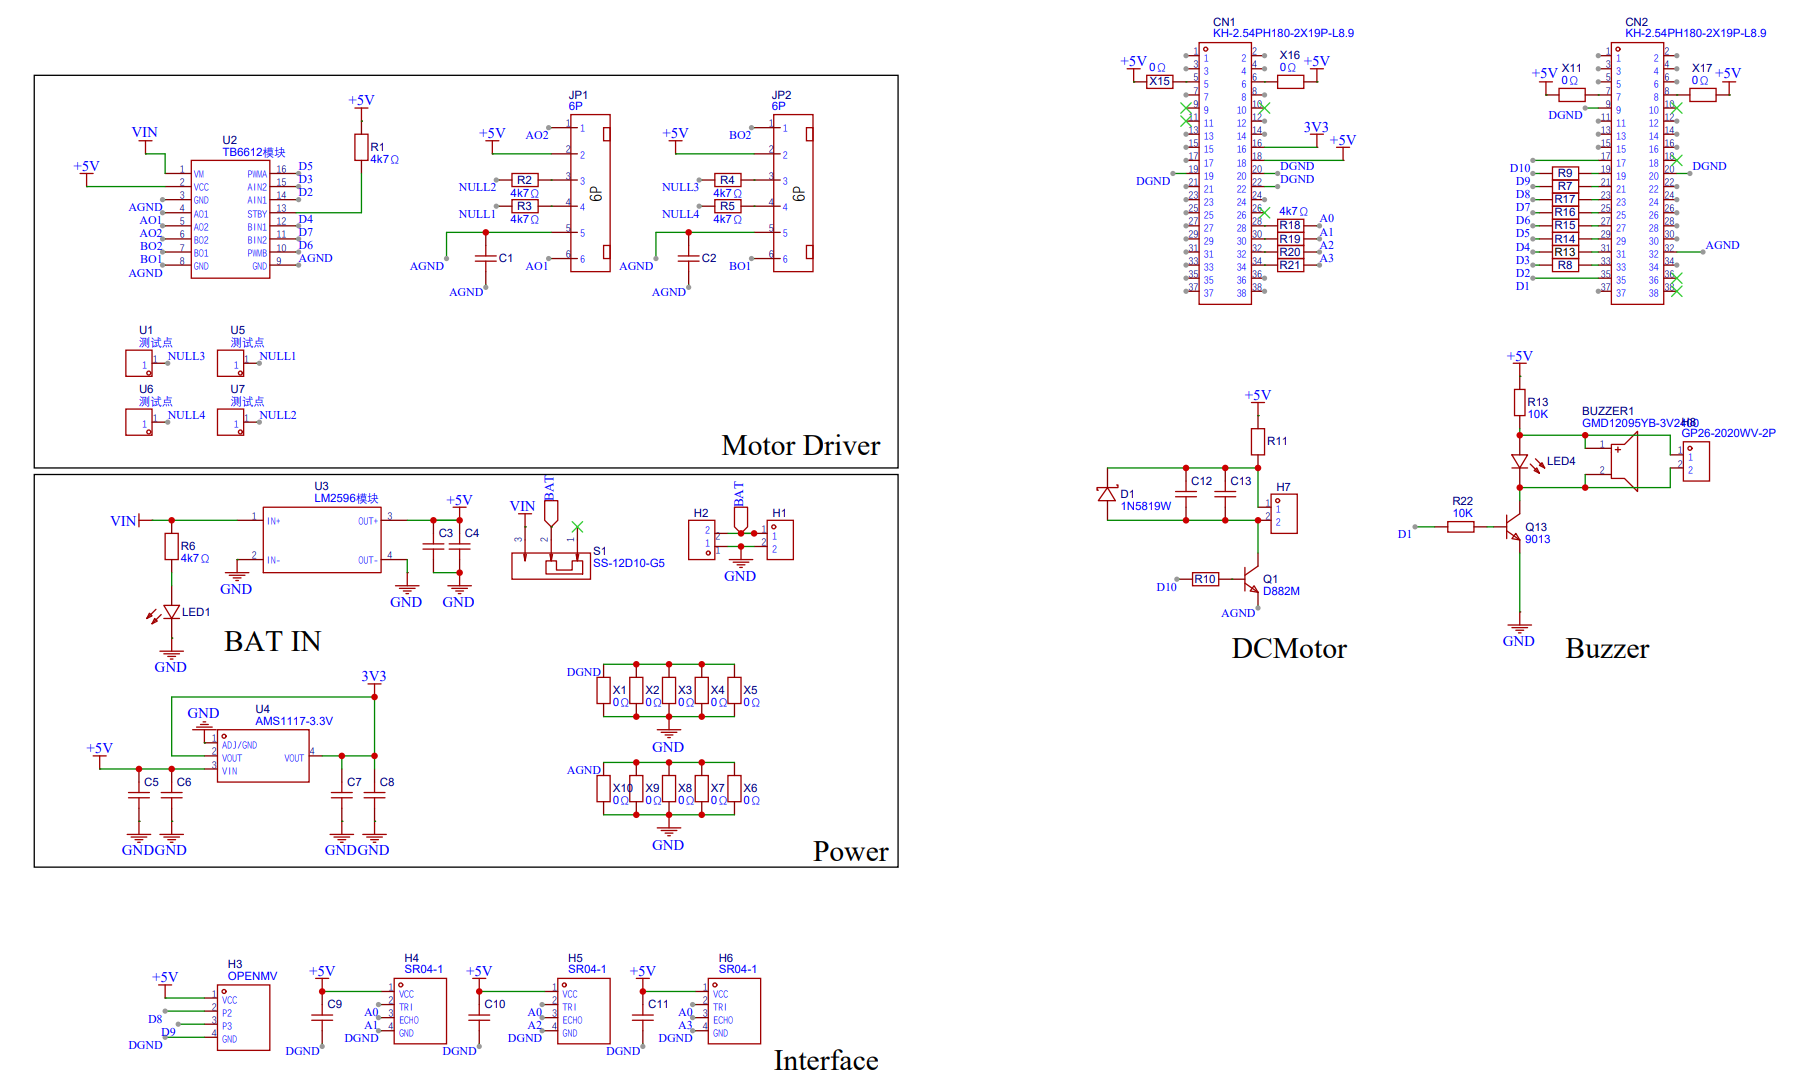
\includegraphics[scale=0.35]{pic/PCB_figure/3_PCB.png}
	\caption{The complete schematic diagram of all components on PCB}
    \label{fig:pcb3}
\end{figure*}

\subsubsection{STM32}
Considering that STM32 was usually separately programmed and adjusted, for convenience, we did not choose to directly solder the STM32 on the PCB, instead, two sets of female headers were used to act as a mediate component between the STM32 and the PCB board. The schematic diagram of these two sets of female headers is shown in Figure \ref{fig:pcb4}, connections of used pins were clearly defined.

\begin{figure*}[!h]
	\centering
	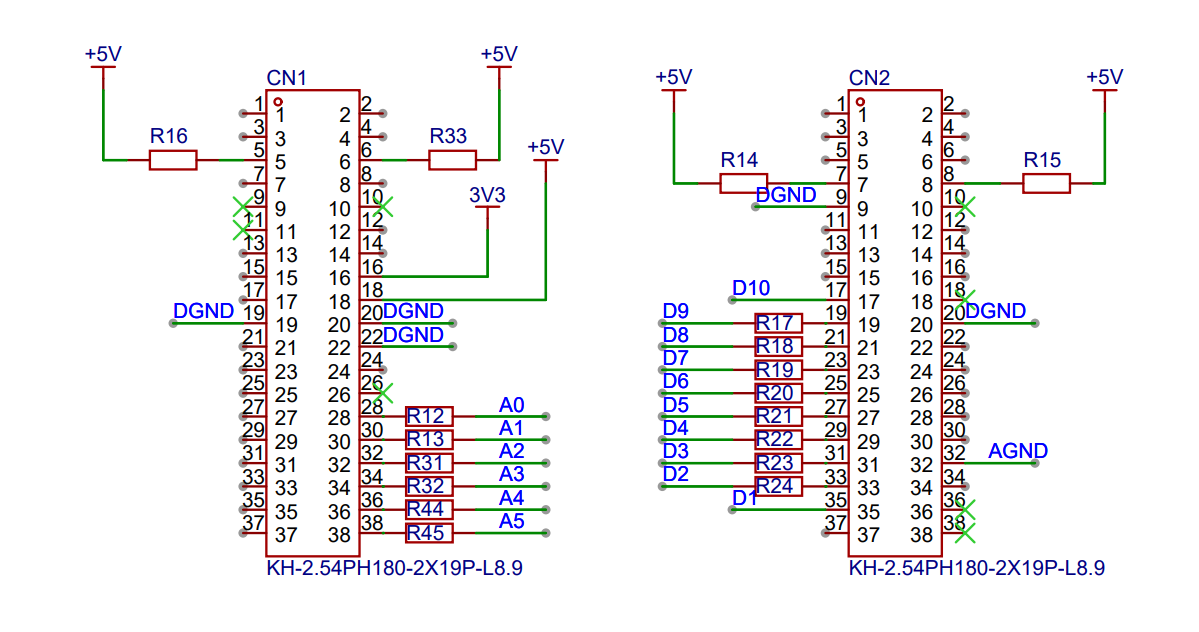
\includegraphics[scale=0.34]{pic/PCB_figure/4_PCB.png}
	\caption{The two sets of female headers to carry the STM32}
    \label{fig:pcb4}
\end{figure*}

\noindent
Once needed to be assembled onto the PCB, the STM32 could be directly plugged into the female headers while when required to be programmed alone, it also can be easily extract from them.
\subsubsection{Motor Drive}
In motor driver part, shown in Figure \ref{fig:pcb5}, a TB6612 chip module was used to power the motors of wheels and the fan. Two female headers are used to connect the wheels. Four test points were used for test in assemble processes and act as extra connection pins.

\begin{figure*}[!h]
	\centering
	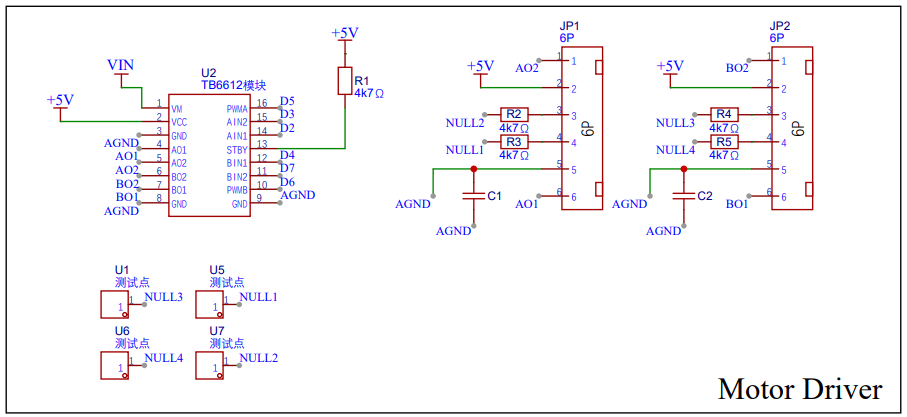
\includegraphics[scale=0.6]{pic/PCB_figure/5_PCB.png}
	\caption{The schematic diagram of Motor Driver}
    \label{fig:pcb5}
\end{figure*}

\subsubsection{Power}
As for power supply, shown in Figure \ref{fig:pcb6}, two DC to DC converters were used and a switch was used to control the power cut off. Two sets of pins with different directions are used to provide connection to battery. The use of different directions is to make sure the connection can be compatible with various kinds of batteries. Besides, two sets of parallel resistors were used to prevent high frequency noise from the ground signal. 

\begin{figure*}[!h]
	\centering
	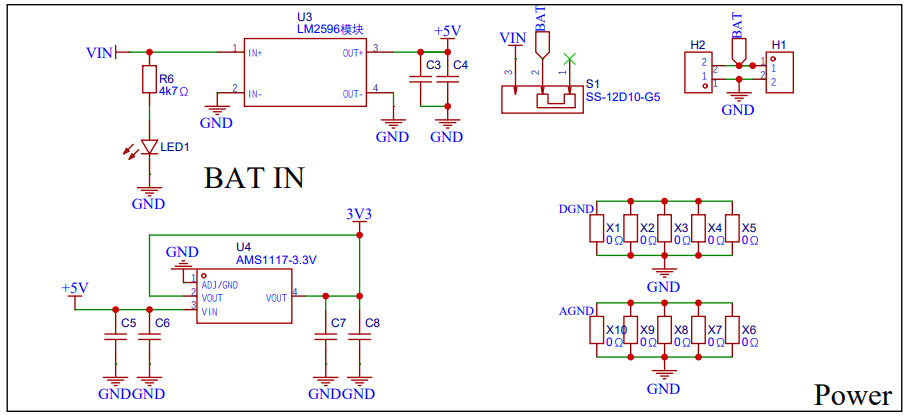
\includegraphics[scale=0.6]{pic/PCB_figure/6_PCB.png}
	\caption{The schematic diagram of Power block}
    \label{fig:pcb6}
\end{figure*}

\subsubsection{OpenMV and ultrasonic modules}
OpenMV and the ultrasonic modules used in this project were required to have specific angle and distance with the task props. Therefore, it is not suitable to soldering them directly on the PCB, as an alternative, connecting interfaces soldered on PCB were used to connect the OpenMV and ultrasonic modules. The schematic was shown in Figure \ref{fig:pcb7}
\begin{figure*}[!h]
	\centering
	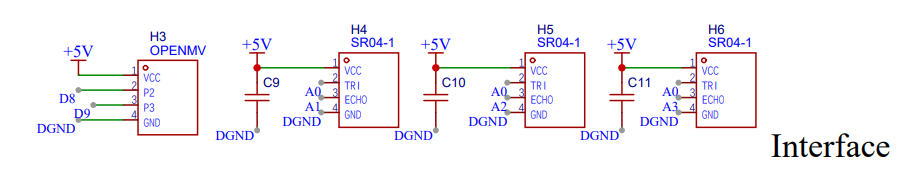
\includegraphics[scale=0.6]{pic/PCB_figure/7_PCB.png}
	\caption{The schematic diagram of interfaces for OpenMV and ultrasonic modules}
    \label{fig:pcb7}
\end{figure*}
\subsubsection{Buzzer and LED}
A buzzer and several LEDs were used to indicate whether the circuit on the board is working properly as we expected. And these devices are soldered on the PCB directly along with the passive devices. Their schematic diagram is shown as blow in Figure \ref{fig:pcb8}
\begin{figure*}[!h]
	\centering
	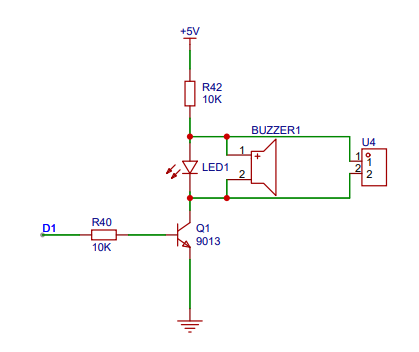
\includegraphics[scale=0.7]{pic/PCB_figure/8_PCB.png}
	\caption{The schematic of a buzzer and a LED}
    \label{fig:pcb8}
\end{figure*}
\subsubsection{Layout arrangement}
After finishing the work in schematic diagram, the devices were transformed from the schematic diagram into real form packaging on PCB. Then, arrange the devices on the space of the PCB, make the arrangement neatly, has a high space-use efficiency and avoid cross line as possible. Figure \ref{fig:pcb9} gives an example of arranging the devices.

\begin{figure*}[!h]
	\centering
	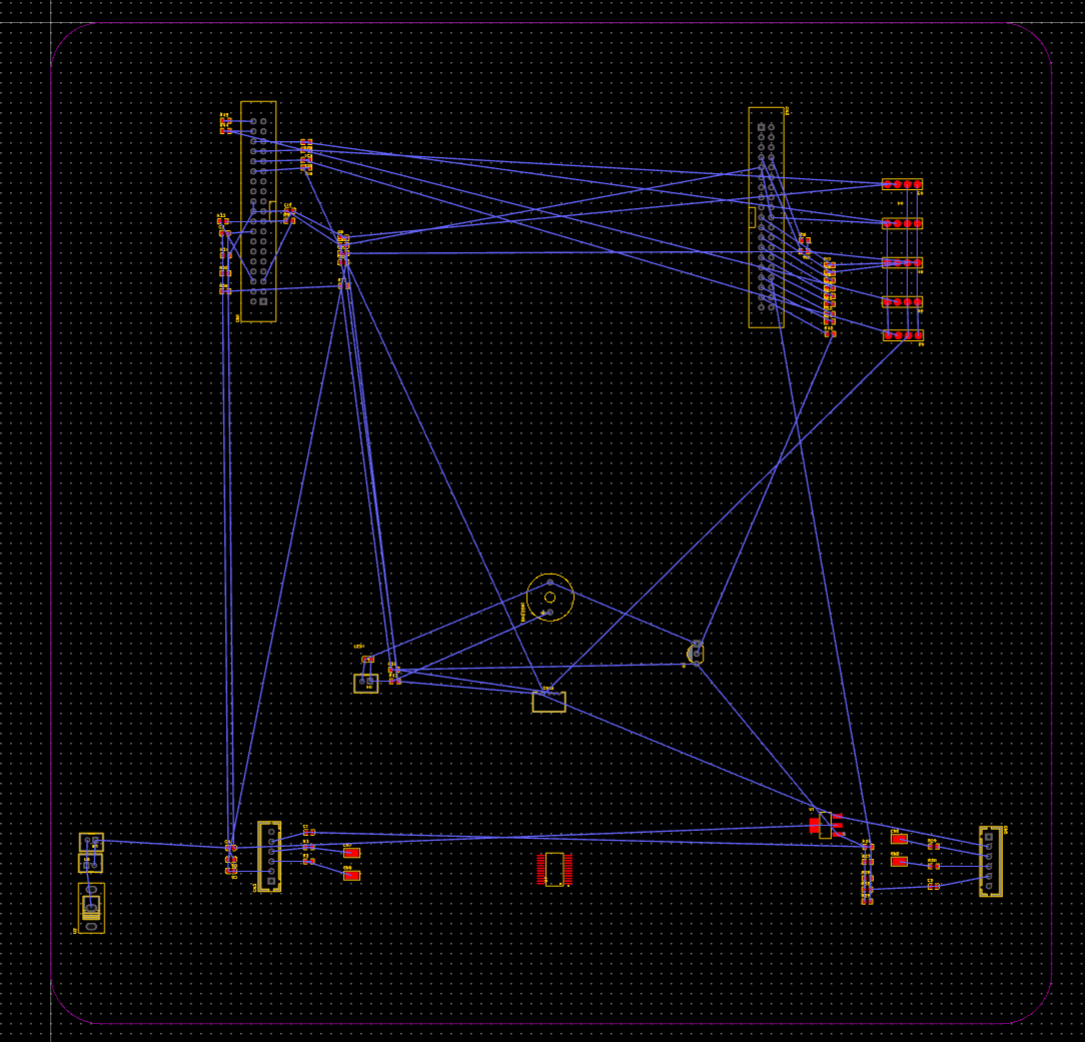
\includegraphics[scale=0.43]{pic/PCB_figure/9_PCB.png}
	\caption{An example of arranging devices on a PCB}
    \label{fig:pcb9}
\end{figure*}

\subsubsection{Wiring and interconnection}
After the arrangement, all the devices need to be connected following the instruction lines to generate proper signal, power and ground signals. Before connecting, specific rules can also be defined and Figure \label{fig:pcb10} gives an example of connecting through wires, vias or copper layer. At last, all devices were connected properly among 4 layers by applying various types of connecting methods.
\begin{figure*}[!h]
	\centering
	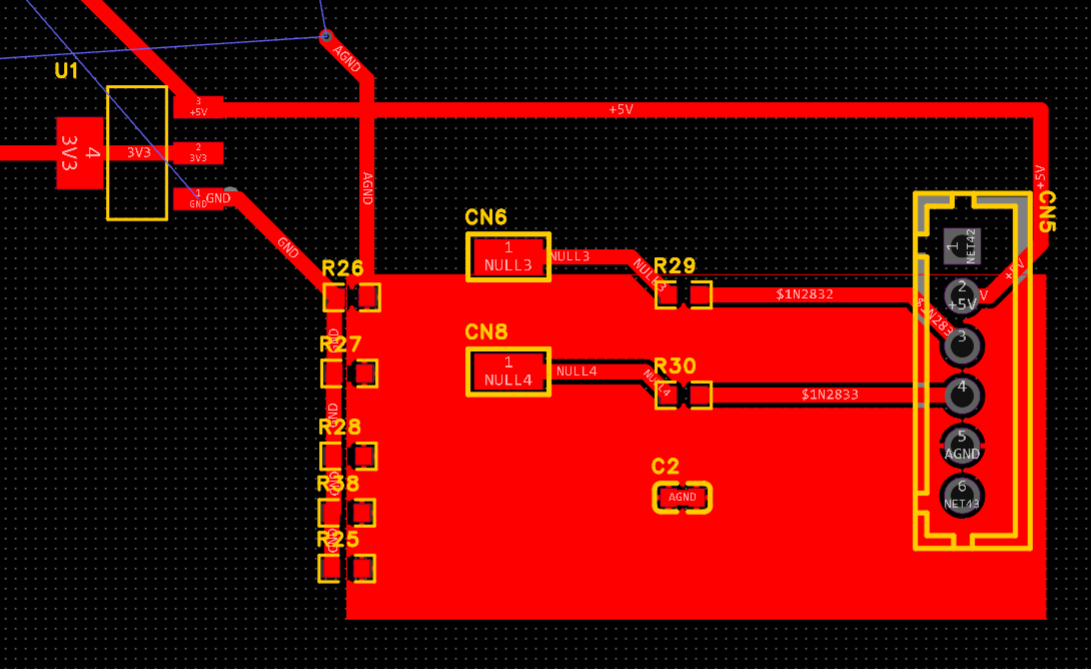
\includegraphics[scale=0.28]{pic/PCB_figure/10_PCB.png}
	\caption{ An example of connections on a PCB}
    \label{fig:pcb10}
\end{figure*}
\subsubsection{Adding silk screen painting}
Silk screen painting is descriptive signs on the top layer, it gives comments, instruction or identification on a PCB board. Figure \label{fig:pcb11} gives an example of adding silk printing on our PCB board and how it looks like in a 3D view.
\begin{figure*}[!h]
	\centering
	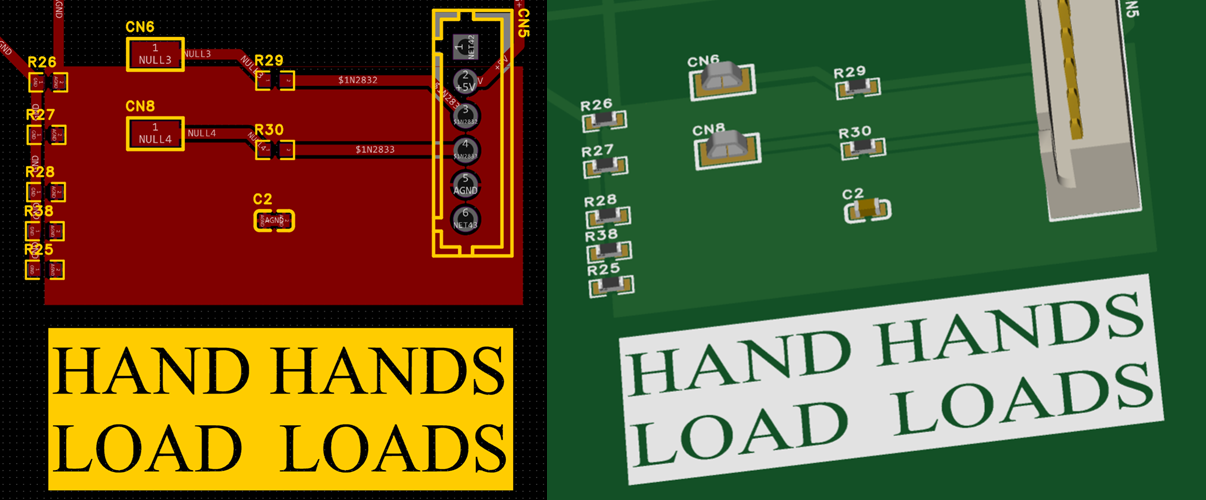
\includegraphics[scale=0.25]{pic/PCB_figure/11_PCB.png}
	\caption{An example of adding silk printing and its 3D view}
    \label{fig:pcb11}
\end{figure*}
\subsubsection{Final result}
After all the design work was done, perform the design rule check (DRC) to make sure all the design was properly obeying the defined rule and fix any error that find in the check. Finally, the correct design files can be exported as Gerber files and sent to the factory. The final designed PCB board is shown in Figure \ref{fig:pcb12}.
\begin{figure*}[!h]
	\centering
	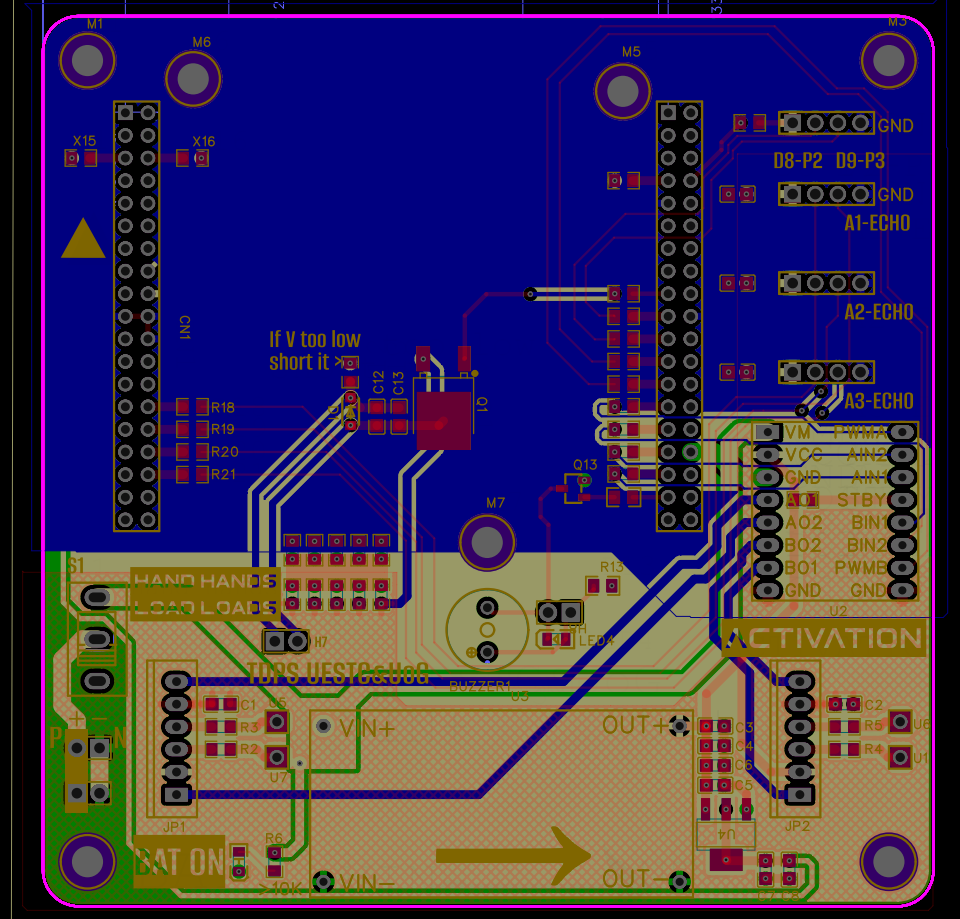
\includegraphics[scale=0.3]{pic/PCB_figure/12_PCB.png}
	\caption{The final complete PCB design}
    \label{fig:pcb12}
\end{figure*}
\subsection{Assemble Part}
In assemble part, it was mainly focused on the fabricated PCBs and the elements received from outsourcing factory. The received raw PCB cannot be directly used in our smart vehicle but after adding all required components on it. Figure \ref{fig:pcb13} shows the bare PCB with no extra components added on it.
\begin{figure*}[!h]
	\centering
	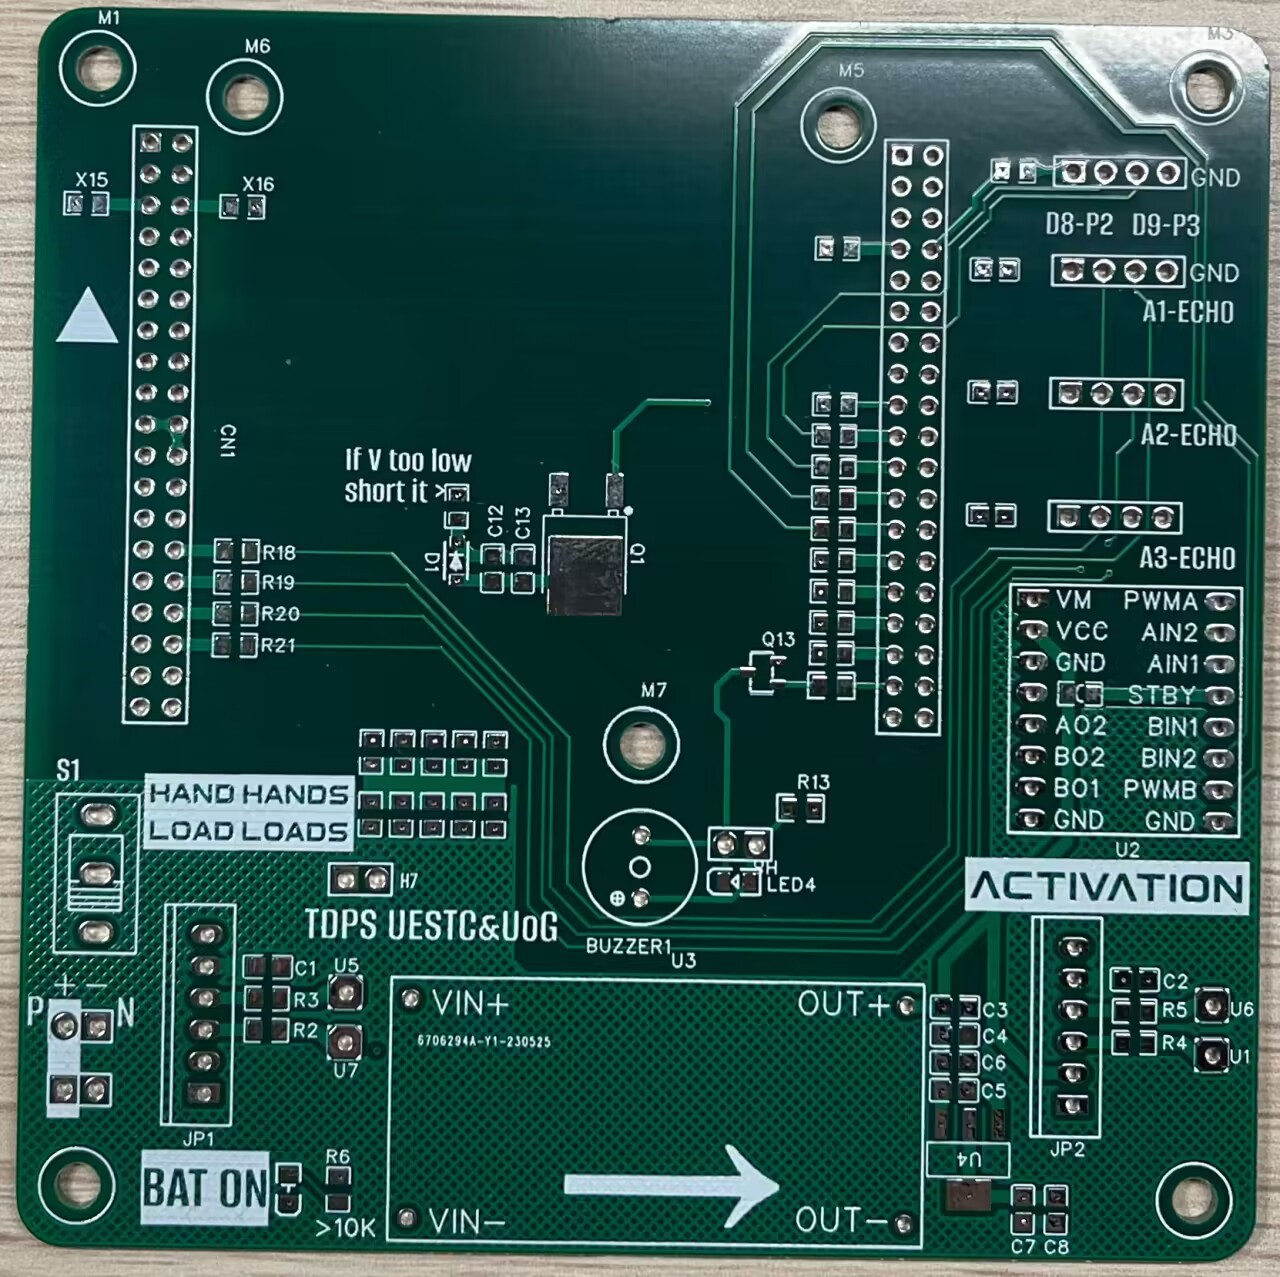
\includegraphics[scale=0.17]{pic/PCB_figure/13_PCB.jpg}
	\caption{Bare PCB board}
    \label{fig:pcb13}
\end{figure*}
\subsubsection{Assembling of passive devices and mediate connectors}
The passive devices that used on our PCB are chip resistors and chip capacitors. Chip resistors and chip capacitors are very thin and tiny devices usually assembled on electrical boards. The processing of assembling chip resistors and capacitors on the PCB can be divided into two steps – (1) add solder paste at needed places and stick the passive devices on it physically; (2) use a heating stage to melt the solder paste, adjust the location of the devices and cool down to form tight bond chemically. Figure \ref{fig:pcb14} gives an example of this process. 
\begin{figure*}[!h]
	\centering
	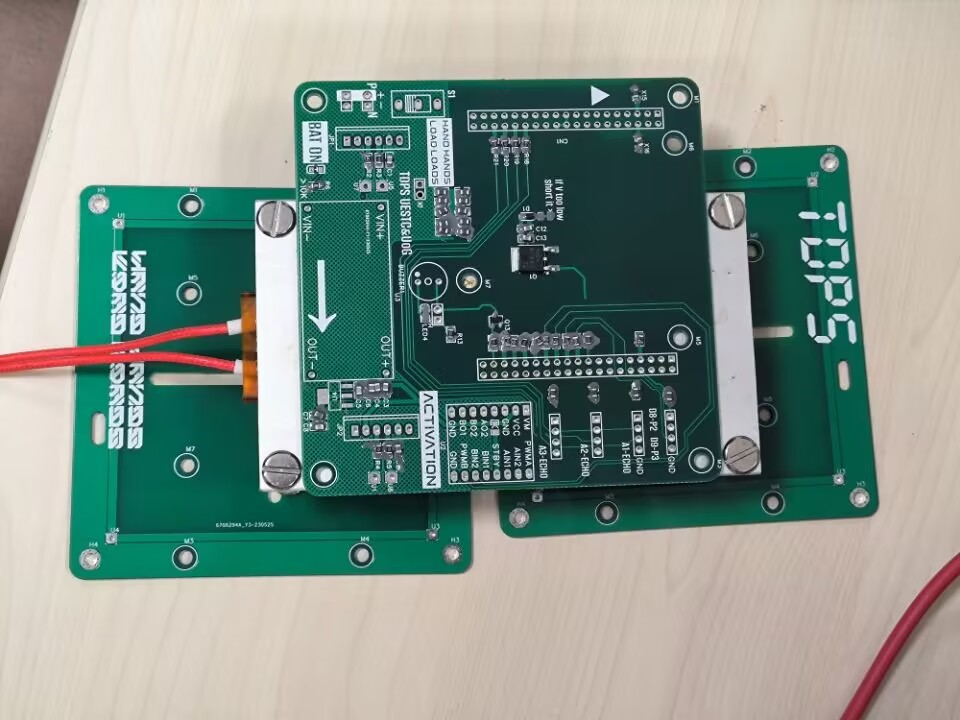
\includegraphics[scale=0.25]{pic/PCB_figure/14_PCB.jpg}
	\caption{An example of passive devices adding process}
    \label{fig:pcb14}
\end{figure*}

\noindent
The mediate connectors used are pin headers and female headers to connect the IC devices. For mediate connectors, their pins were firstly aligned with the via holes on PCB, then a soldering iron was used to heat the pins and the solder was added to form stable connection. The soldered connection was shown in Figure \ref{fig:pcb15}.
\begin{figure*}[!h]
	\centering
	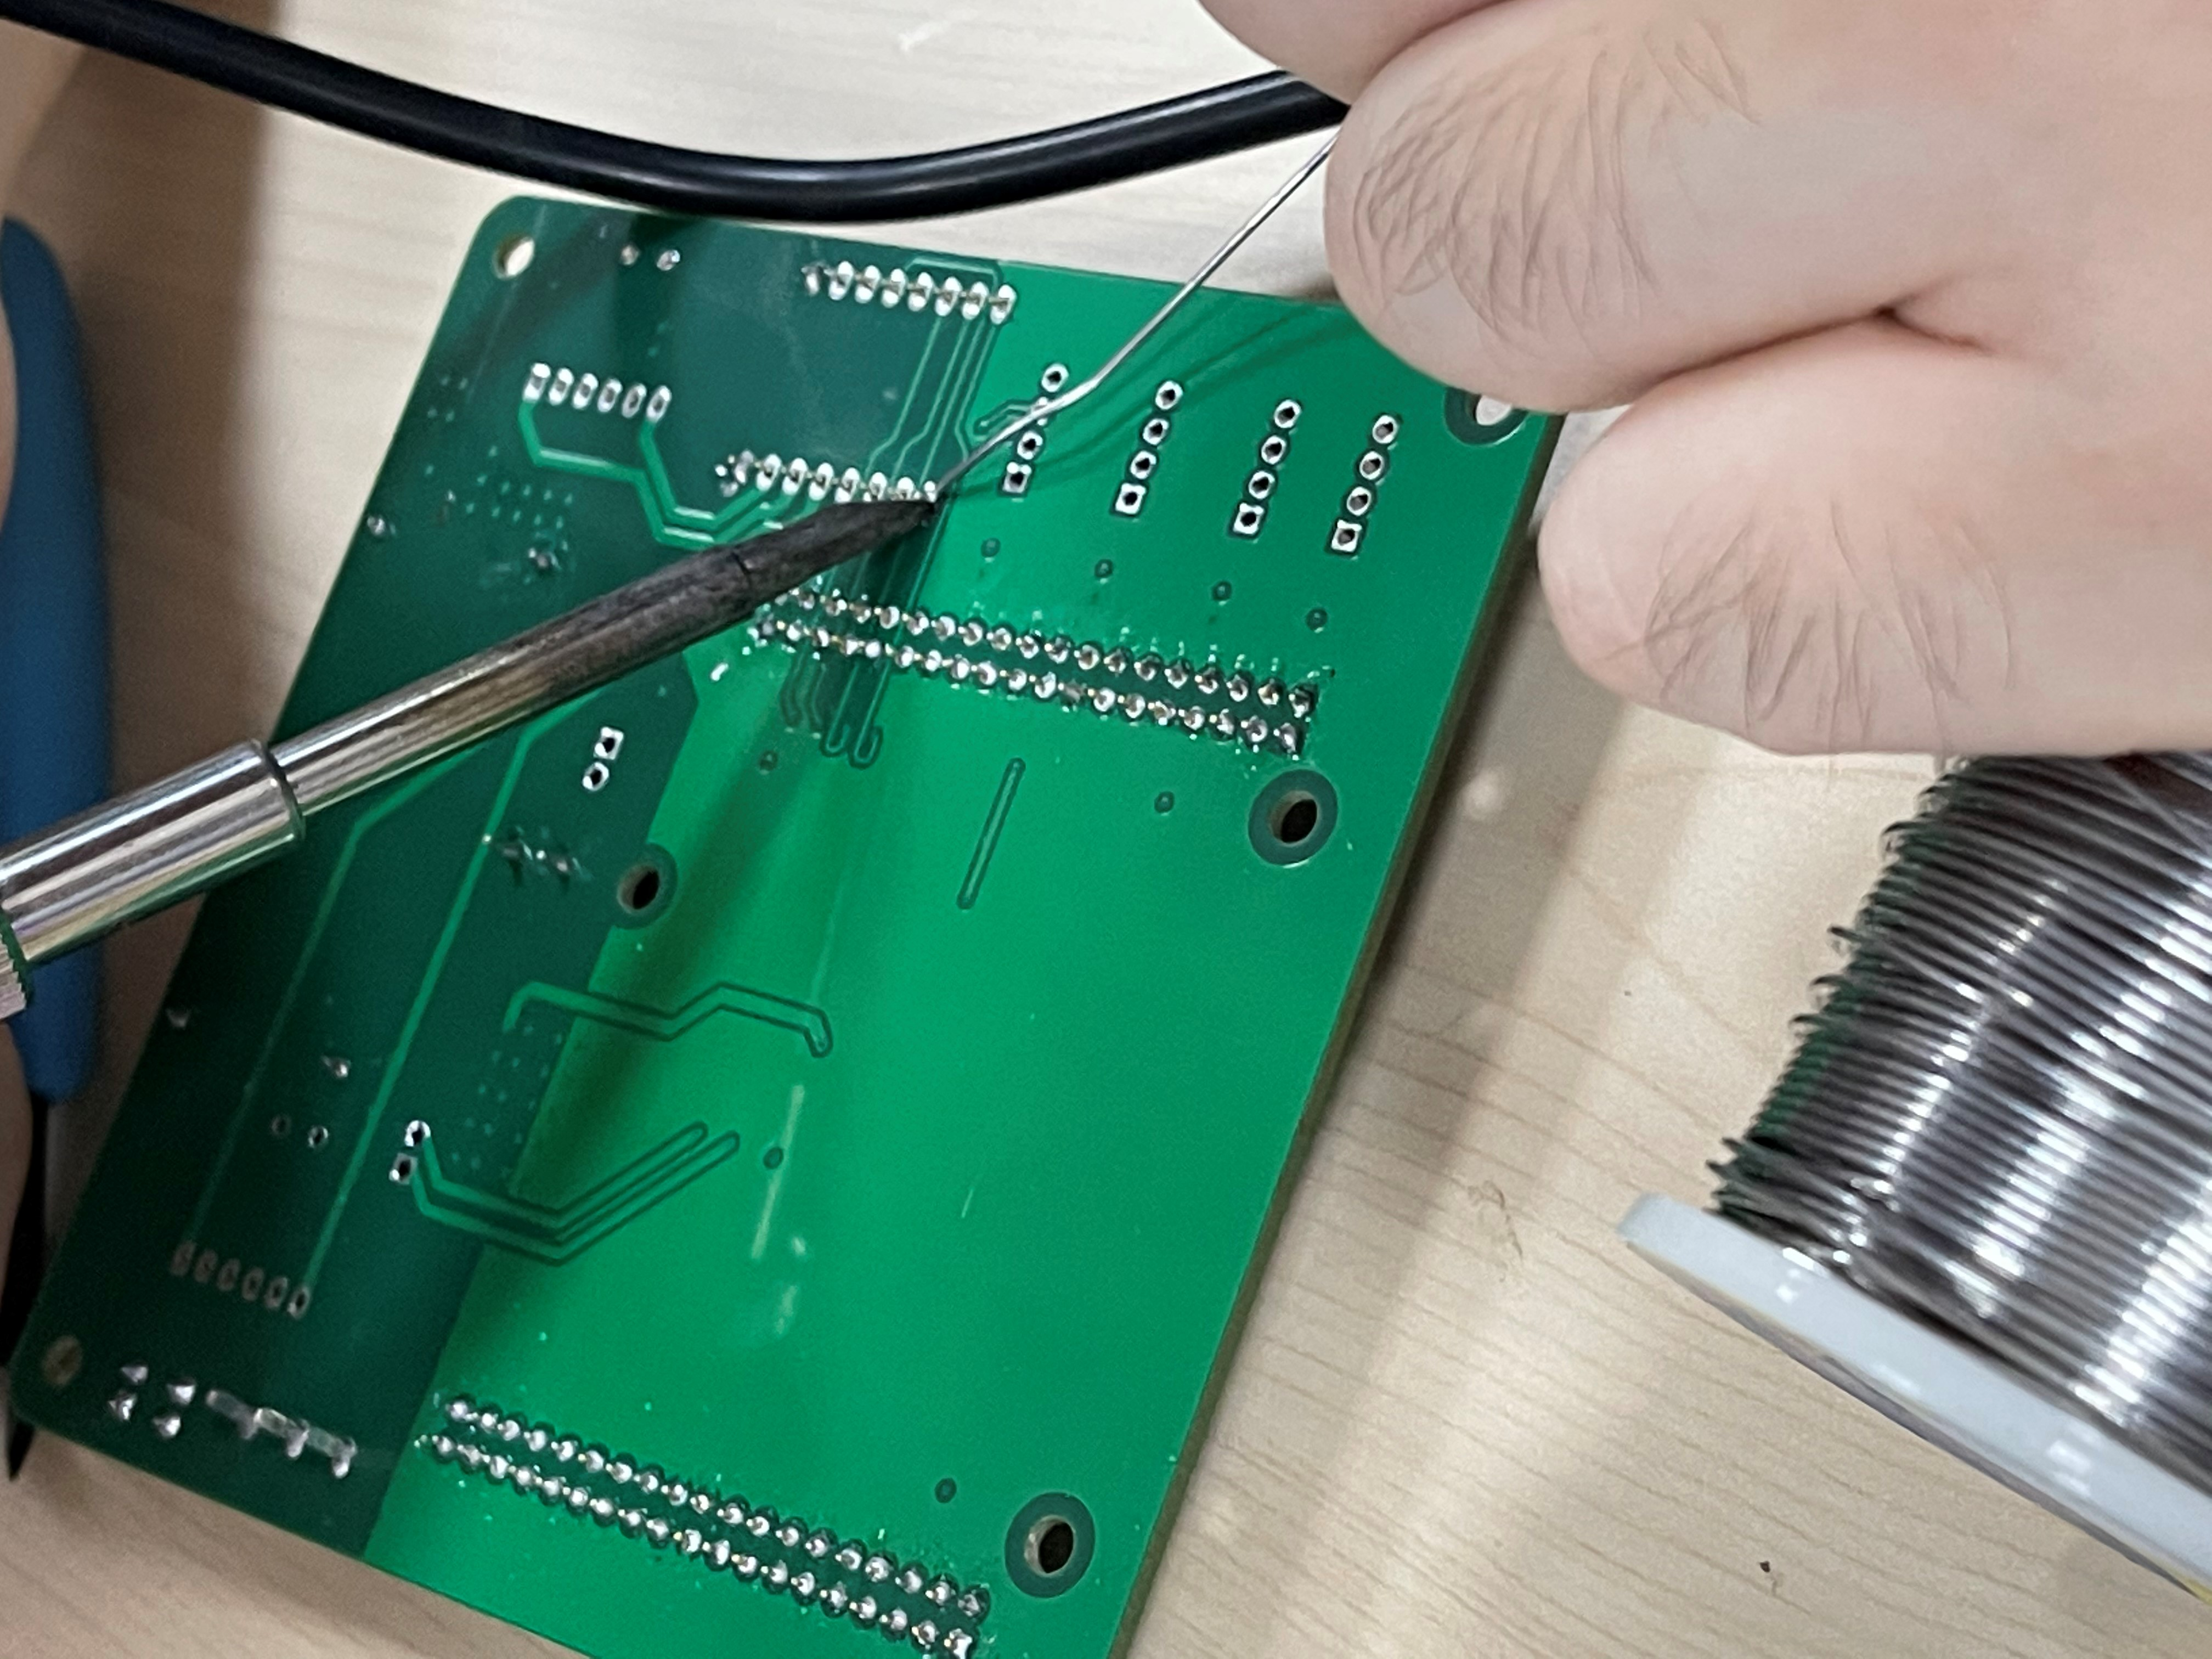
\includegraphics[scale=0.05]{pic/PCB_figure/15_PCB.jpg}
	\caption{Soldering the connection}
    \label{fig:pcb15}
\end{figure*}
\subsubsection{Assembling of functional modules}
After adding passive devices and mediate connectors, the functional modules can finally be assembled on the PCB board. For STM32 and the motor driver chip, they can be directly plugged into the female headers, while for the OpenMV, ultrasonic and Bluetooth modules, they were connected to the PCB board by connecting wires to interfaces on the PCB. And the completed functional PCB board of our smart vehicle was demonstrated in Figure \ref{fig:pcb16}.

\begin{figure*}[!h]
	\centering
	\includegraphics[scale=0.12]{pic/PCB_figure/16_PCB.png}
	\caption{The complete PCB board used in smart vehicle}
    \label{fig:pcb16}
\end{figure*}

\newpage
\section{Communication between Boards}\label{sec:itc}
\colorbox{yellow}{\textbf{Developer:} Lyu Guandong 2614397L}

\subsection{Introduction}
This part presents a comprehensive study on the implementation and usage of Universal Asynchronous Receiver/Transmitter (UART) for serial communication within a miniature autonomous line-tracing vehicle. The primary aim of the project was to establish effective and efficient data transmission between the numerous electronic components within the vehicle, leveraging UART as the key communication protocol.

As an IEEE student major, my work has been guided by the principles of the Institute of Electrical and Electronics Engineers, aiming to foster technological innovation and excellence for the benefit of humanity. The IEEE standards have significantly influenced the design and implementation of this project, ensuring a reliable and optimized data transmission system.

The autonomous line-tracing vehicle is a small-scale model car that uses sensors and control algorithms to trace and follow a specific line path. This function requires a seamless and robust communication between its multiple components, including sensors, microcontrollers, and actuators. In this context, UART was selected due to its simplicity, reliability, and ability to facilitate asynchronous communication between these components, resulting in effective data transmission without the need for a clock signal.

This part is intended to provide an overview of the design, implementation, and performance evaluation of UART-based serial communication within the line-tracing vehicle. It includes an analysis of the communication requirements for the vehicle, reasons for choosing UART, implementation details, challenges encountered during the process, and solutions developed to overcome those.

Furthermore, the report will offer a detailed examination of the data transmission performance, addressing the efficiency of the implemented UART communication protocol. Potential areas of improvement and recommendations for future work will be proposed, aiming to enhance the vehicle's overall performance and reliability.

Overall, this project emphasizes the practical application of theoretical knowledge and IEEE principles to solve real-world challenges in the field of robotics and automation. The ultimate goal of this work is not only to develop an efficient line-tracing vehicle but also to contribute to the broader understanding and application of UART communication within complex electronic systems.

To ensure our car can drive alone the line, we need openmv and stm32 work together.Openmv is responsible for capturing the images of the road and processing the images, and STM32 is responsible for driving the car correctly. This requires the data can be transformed between these two components. The very beginning, we chose a very simple way to tell STM32 which way to go, we used two DigitalOut signals. the openmv will get the angle between the car and the road, and then determine whether the route takes the left or the right side of the car. If the route is on the right, then let one port output high-level and the other output low-level, and vice versa. When the road is as the same direction with the car, then output low-level on both ports. The stm32 can easily receive information in this way, however, this is too stupid for the car because it can only turn left or turn right of fixed angle. Then we tried another way to transmit the information, we directly send the angle to stm32 and use the algorithm in stm32 to determine the difference of speed of motors on different sides. In this way, the small car will become more flexible and steer more accurately. This requires the use of serial communication. We finally chose the UART for the communication because it is easy to use and reliable in this case. Connect Tx and Rx port in openmv with RX and TX port in stm32, ground them and set the same bout rate for this two components. Then we can transmit the data from openmv to stm32. It is worth mentioning that I use variable in string format when transferring data, and use the command atoi to convert it to integer variables after it is received by stm32. In addition, in stm32 we need to define and initialize the registers to store the received data and then call from them.

\subsection{Basic information about UART}
Universal Asynchronous Receiver/Transmitter (UART) is a type of serial communication protocol that's crucial in the field of computer hardware and telecommunications. The simplicity, cost-effectiveness, and ease of implementation have made UART a go-to choice for many low-speed short-distance data transmission needs.

The principle of UART communication revolves around two key elements: the transmitter (which sends the data) and the receiver (which receives the data). Let's delve deeper into the working mechanism of both:
\subsubsection{Transmission}
The transmitting UART first converts the data from parallel to serial form. The data to be transmitted is usually 8-bit, but can be 5, 6, 7, or 9 bits, depending on the system's requirement. Before transmission, a start bit is added at the beginning and one or two stop bits are added at the end of the data. The start bit is always low (or '0') and the stop bit is always high (or '1'). This way, each block of data is surrounded by a start and stop bit, this format is known as a "frame". The addition of these bits allows the receiving UART to recognize when the data bits are being transmitted. The data package transmitted through UART is shown in \ref{com:pac}
\begin{figure}[!h]
    \centering
    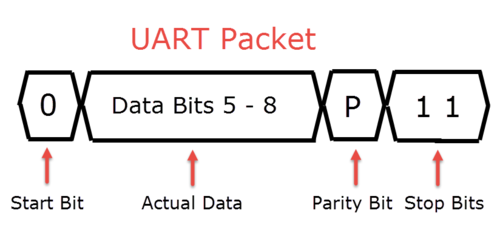
\includegraphics[scale=0.7]{pic/communication/uart1.png}
    \caption{Data Package in UART}
    \label{com:pac}
\end{figure}
\subsubsection{Receiver}
The receiving UART identifies the start bit, collects the data bits, and then stops upon recognizing the stop bit(s). The received serial data is then converted back to parallel data.

The term "asynchronous" in UART means that it doesn't require a clock signal to synchronize the sending and receiving units. Instead, both units must agree on the data rate before communication begins. This rate is known as the baud rate and it signifies the speed at which data is transferred. For example, a baud rate of 9600 means 9600 bits are sent per second.

UART also supports full-duplex communication, which means data can be transmitted and received simultaneously. This is made possible by using two data lines - Transmit Data (TX) and Receive Data (RX).

Error detection is another key feature of UART. It has a parity bit for basic error detection. This bit is set (either to '1' or '0') in the transmitter depending on the number of logic 1's in the data to make the total number of 1's either even (for even parity) or odd (for odd parity). The receiver checks this bit to detect if any bit errors have occurred during transmission.

In our autonomous line-tracing vehicle project, the microcontroller uses UART to communicate with the various components. Data from the line-tracking sensor is sent to the microcontroller through UART, and the microcontroller sends control signals to the actuators (like motors) in the same way. The consistent and efficient two-way communication facilitated by UART ensures the vehicle can smoothly trace the line.

\subsection{Circuit Connection between Boards for UART}
The Universal Asynchronous Receiver/Transmitter (UART) protocol requires minimal connection to facilitate communication between two boards, such as microcontrollers. Usually, only three wires are necessary: one for transmitting data (TX), one for receiving data (RX), and a common ground reference (GND).
\begin{itemize}
    \item TX: This pin is used for transmitting data. The TX pin of the first board is connected to the RX pin of the second board
    \item RX: This pin is used for receiving data. The RX pin of the first board is connected to the TX pin of the second board
    \item GND (Ground): Both boards need to share a common ground. Therefore, connect the GND pin of the first board to the GND pin of the second board
\end{itemize}

Thus, the data transmission flow would be: Board 1 TX $\rightarrow$ Board 2 RX and Board 1 RX $\leftarrow$ Board 2 TX.

In our autonomous line-tracing vehicle, the microcontroller (STM32) communicates with sensors and actuators using UART. The RX, TX, and GND pins of the microcontroller would connect to the respective TX, RX, and GND pins on the sensors or actuator control boards.

Lastly, proper software setup on both boards is crucial to specify the baud rate, parity, and stop bits. Both boards must use the same configuration to communicate properly.

\subsection{Communication Between STM32 and Openmv}
STM32 and OpenMV are powerful microcontrollers that can communicate with each other through the UART protocol. STM32 is typically used for real-time applications due to its exceptional performance and broad range of features, while OpenMV is designed for machine vision applications, providing built-in image processing capabilities.

In the context of our autonomous line-tracing vehicle, the OpenMV camera detects the line to be traced and calculates the angle between its heading direction and the line. This angle is then communicated to the STM32 microcontroller, which adjusts the vehicle's path accordingly.

The communication between the two boards is achieved through UART, as follows:
\begin{itemize}
    \item The OpenMV board calculates the angle between its heading direction and the line. This angle is stored in a string variable
    \item The OpenMV board then sends this string variable through its TX pin. The UART communication is set at a baud rate of 9600
    \item The transmitted data travels along the connected wire to the RX pin of the STM32 board
    \item Upon receiving the data, the STM32 microcontroller parses the string to extract the angle
    \item Based on this angle, the STM32 board makes necessary adjustments to the direction of the motors of the vehicle, aligning it properly with the line
\end{itemize}

The results of this communication are evident in the accurate line-tracing capabilities of the vehicle. The continuous feedback from the OpenMV board enables real-time adjustments to the vehicle's path, making it adept at following even complex, curving lines. Compared with the Plan A, this control system is much more flexible and accurate.

The choice of a 9600 baud rate provides a balance between speed and error resistance in the transmission. While higher baud rates could transmit data faster, they may increase the chance of transmission errors. Conversely, slower baud rates may provide fewer errors but might not be able to keep up with the real-time nature of the vehicle's requirements. Hence, 9600 is a commonly chosen baud rate that provides a good trade-off between speed and reliability.

Through this UART-based communication, the combination of STM32 and OpenMV allows the autonomous line-tracing vehicle to function reliably and effectively.

\subsection{Communication between Openmv and HC-12}
In this specific application, we are using the HC-12 to wirelessly transmit data from the OpenMV camera module to a computer. The data sent includes the present time captured by the OpenMV, as well as the information of the group members working on the project.

Here is the basic setup for the communication:
\begin{itemize}
    \item The OpenMV board obtains the present time and the relevant group member information, and packs this data into a string variable
    \item This string is then sent from the OpenMV to the HC-12 module using UART at a pre-agreed baud rate (9600 bps)
    \item The HC-12 module then wirelessly transmits this data to a corresponding HC-12 module connected to the computer
    \item The computer-based HC-12 receives the data and sends it to the computer through a USB-UART bridge (since computers typically do not have a UART interface)
    \item The computer can then display or process the received data, which includes the present time captured by the OpenMV and the group member information
\end{itemize}

The circuit between HC-12 and Openmv is shown in \ref{hc12-cir}

\begin{figure}[!h]
    \centering
    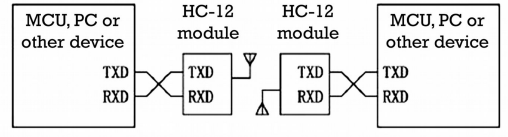
\includegraphics{pic/HC12/hc12-3.png}
    \caption{Ciruit Connection for HC-12}
    \label{hc12-cir}
\end{figure}

The successful result of this communication would be the accurate and timely reception of the data string at the computer end, with all the included information intact. The setup allows for real-time wireless transmission of data between the line-tracing car and the computer, facilitating monitoring and control.

Finally, it's important to note that error checking mechanisms are essential to ensure the integrity of the transmitted data. In a typical UART setup, this is often achieved through the use of parity bits, although other error detection methods can also be employed.
\begin{figure}[H]
    \centering
    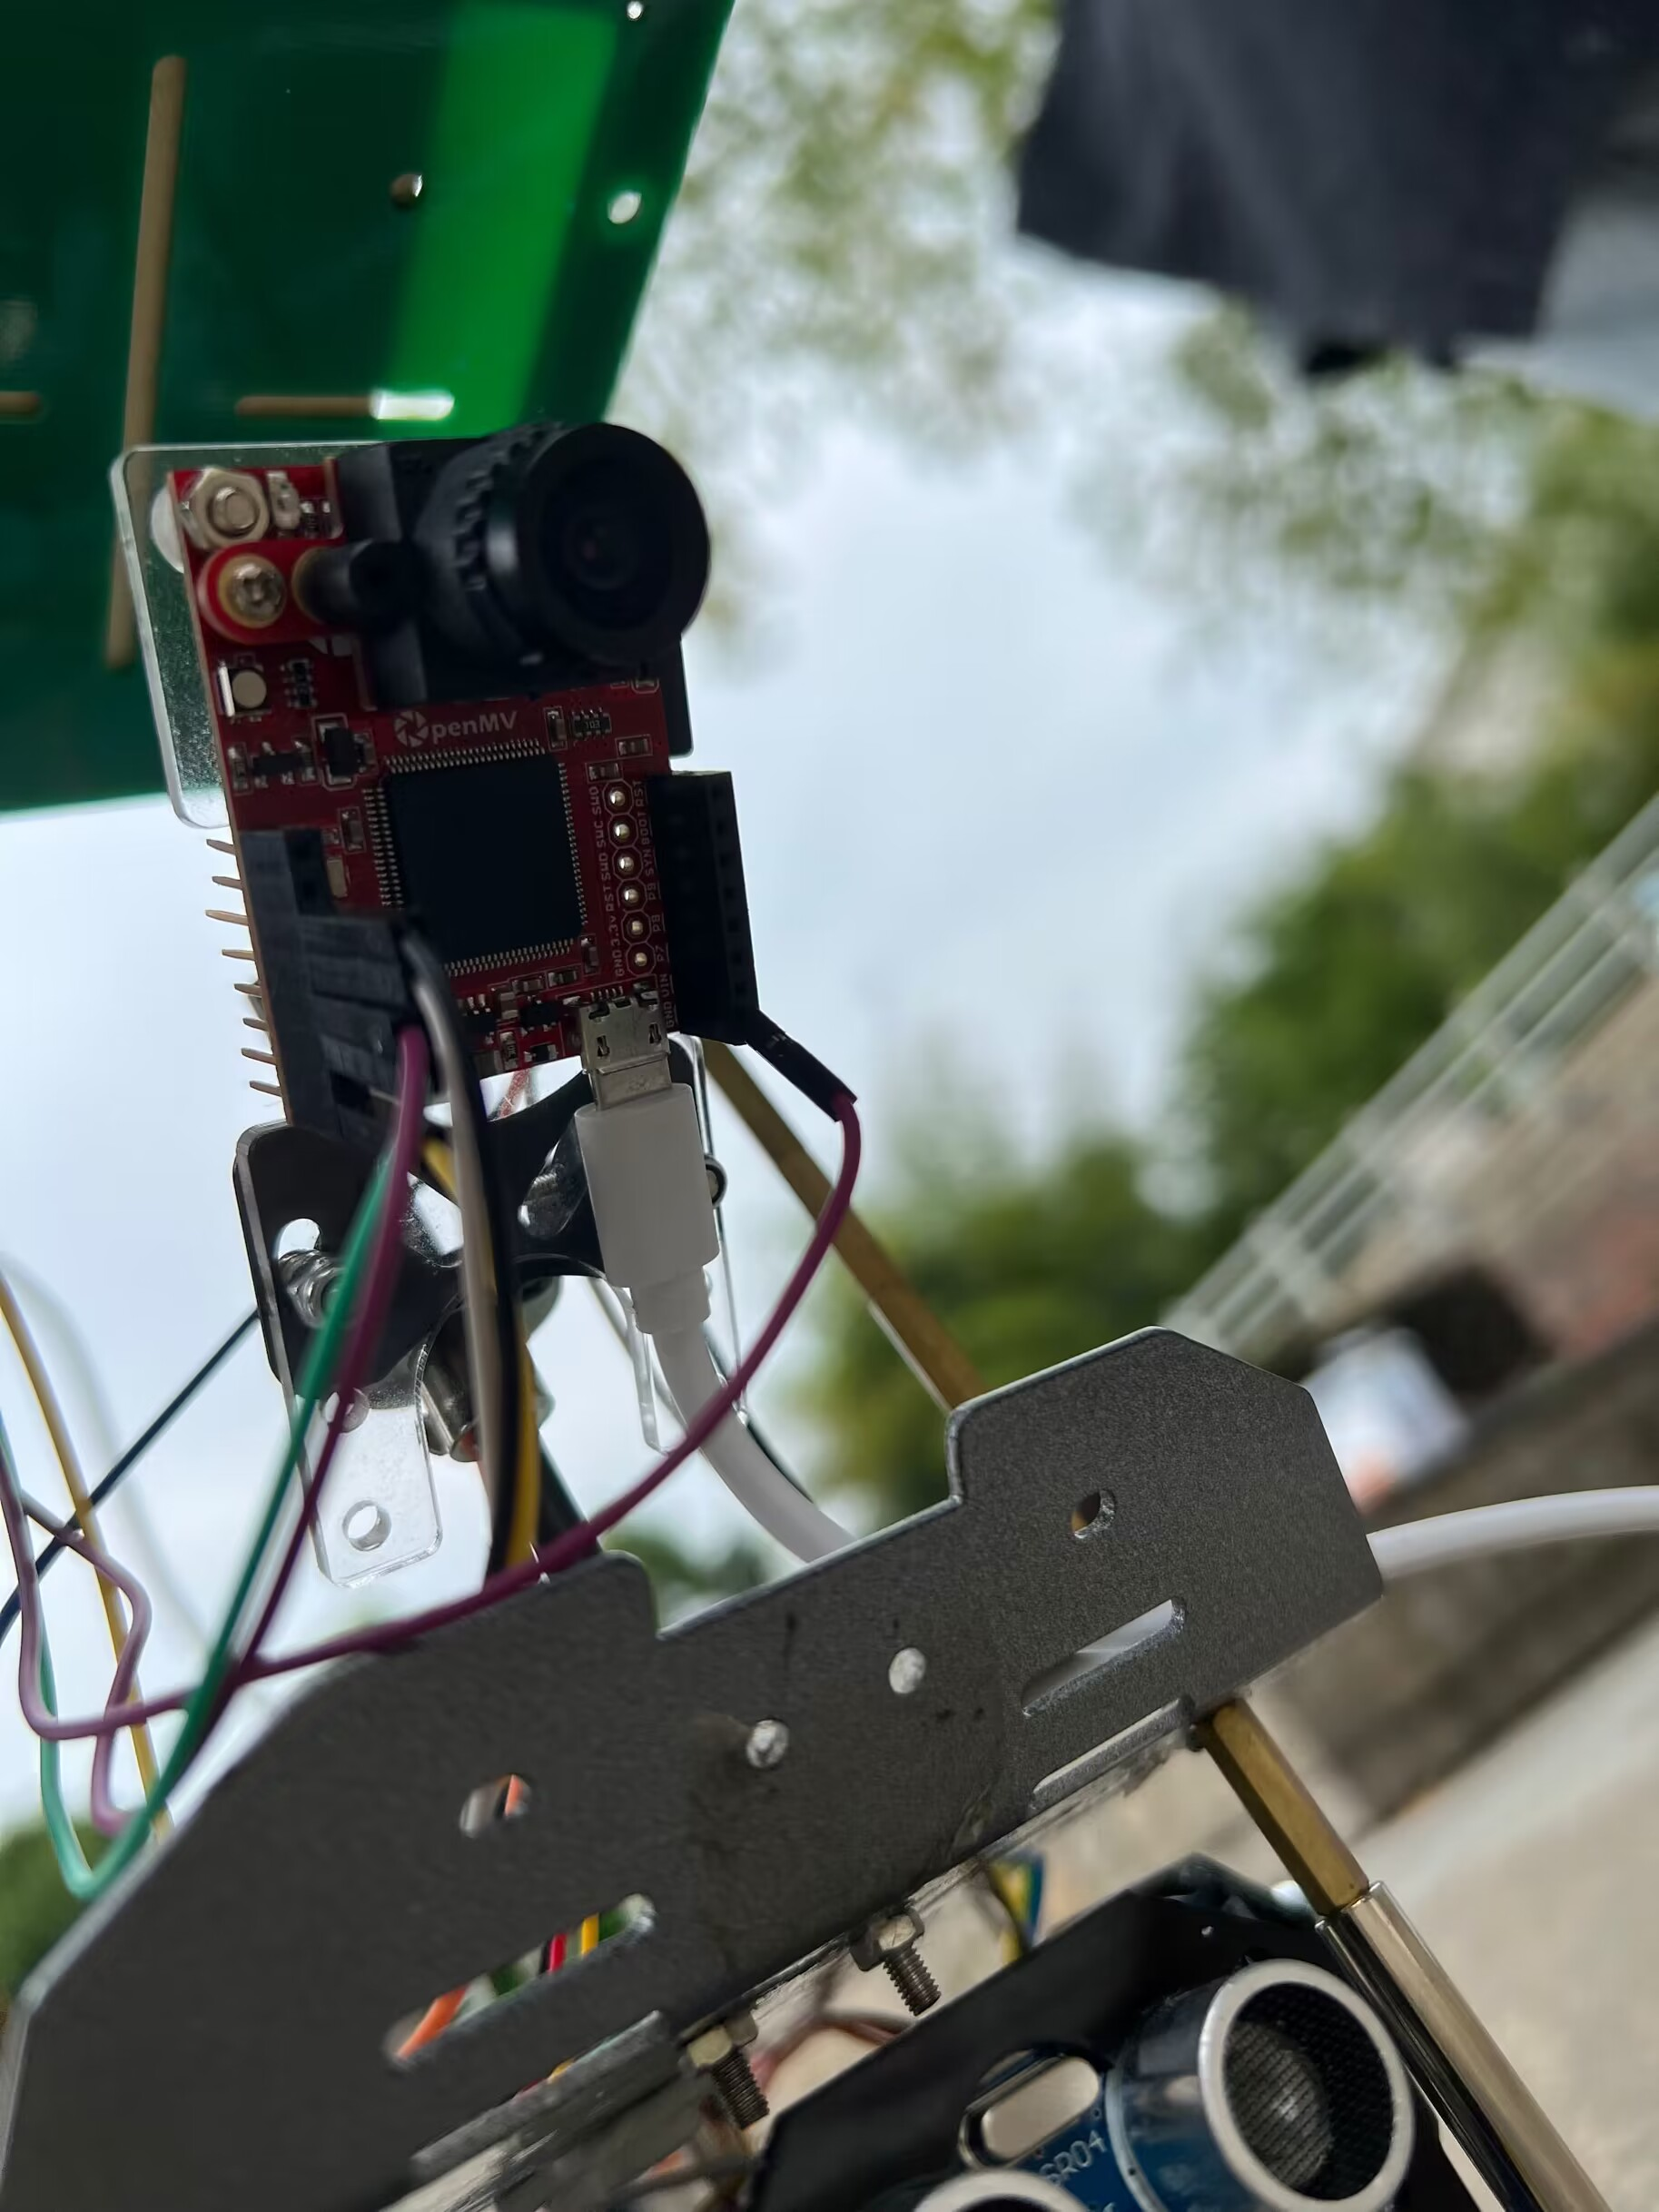
\includegraphics[scale=0.1]{pic/communication/uart3.png}
    \caption{Real Circuit Connection}
    \label{cir-real}
\end{figure}

\newpage
\section{Track Recognition and Tracing}\label{sec:Tracing}
\colorbox{yellow}{\textbf{Developer:} Bi Bodong 2613939B}

\subsection{Introduction}	
In this section, my task is to utilize OpenMV to detect paths in Patio1 and transform them into variables that can be understood and processed by computers. The objective is to achieve a high level of robustness, demonstrating good performance across different positions on the road. To accomplish this goal, I have designed two image preprocessing methods in advance and ultimately selected one of them. For the final variable transformation, I opted to employ a linear regression algorithm. In the following, I will provide a detailed explanation of my contributions.
    
subsection{OpenMV}
The OpenMV Smart Machine Vision Module is a low-power microcontroller processor board that can achieve various visual recognition effects. After integration into the OpenMV, the entire chip has a total of 16 pins, including nine signal transmission pins, a 3.3V power supply pin, a reset pin, a boot pin, a frame sync bit, a power supply port, and a ground port. It is also equipped with 4 built-in LEDs, one red, one green, one blue, and a reverse LED. Additionally, it comes with an SD card slot that supports a maximum of 2GB. The OpenMV Cam also has a built-in RPC (Remote Python/Program Call) library, allowing users to easily connect the OpenMV Cam to a computer, SBC (such as Raspberry Pi), or microcontroller (such as Arduino).
    
Furthermore, with this small module version, users can conveniently program the OpenMV in Python using the compiler provided by the MicroPython operating system, instead of using complex languages like C or C++. This makes it easier for users to handle complex machine vision algorithms and work with high-level data structures. Additionally, users have full control over the OpenMV camera and its inputs and outputs. They can freely capture photos and videos, record, and identify the external environment.
     
\subsection{Digital Image Processing}
Digital image processing skills are the fundamental theories for extracting effective information from images. This information will be used in later procedures for direction identification. The specific methods employed include grayscale processing, binarization, erosion, and robust linear regression.
    
\subsubsection*{grayscale operation}
Based on our on-site investigation of patio 1, we found that some paths have colors that are very similar to their surroundings, making it difficult for OpenMV to distinguish them solely based on RGB information. Additionally, the accuracy of route identification is greatly affected by weather conditions, leading to performance fluctuations. Moreover, RGB images contain a large number of features, and processing such features with OpenMV would require more time. This can result in vehicles being unable to provide timely and accurate feedback on road information. Therefore, before processing the images from the camera, they are converted into grayscale images.
The conversion formula for transforming RGB images into grayscale is as follows:
\begin{tcolorbox}
$$\text{Grayscale value} = 0.299 \times \text{R} + 0.587 \times \text{G} + 0.114 \times \text{B}$$
\end{tcolorbox}
Where R denotes red value, G denotes Green value, B denotes Blue values

Grayscale images carry less color information, and we do not solely rely on this information, providing convenience for subsequent processing stages.
    
\subsubsection*{Binarization}
Considering the future processing needs, the gray-scale image should be converted into a binary image that contains only pure white and pure black colors. In other words, the binary image only has two gray-scale values, namely 0 and 255. When binarizing the gray-scale image pixels, a threshold gray-scale value is used. Pixels with a gray-scale value higher than the threshold are adjusted to 255, while those with a gray-scale value lower than the threshold are set to 0.

This process is necessary and inevitable because the path angle calculation methods can only handle binary images.

Through continuous experimentation and adjustment, we have ultimately chosen to use a threshold parameter of 95. This means that color blocks with a gray-scale value higher than 95 are considered as 255, while color blocks with a gray-scale value lower than 95 are considered as 0. We have also applied the invert operation, which converts white blocks to black blocks. There are two reasons for doing this: it facilitates debugging, and it reduces the impact of brightness changes caused by weather variations on the gray-scale image.

\subsubsection{Dilatation and Erosion}
To obtain effective data and eliminate outliers, a scheme of erosion followed by dilation was used. This functionality is based on the built-in functions of OpenMV, as shown below:

\begin{lstlisting}[language=Python]
Image.dilate(2)
Image.erode(2)
\end{lstlisting}

The principle of erosion is to remove smaller white independent blobs in a black-and-white binary image using image convolution. This effectively eliminates outliers. On the other hand, dilation, also implemented using convolution, enlarges the white pixels in the image, significantly increasing the road-related information. The resulting effect, as shown in the Figure \ref{fig:tr}, is highly significant.

\begin{figure}[H]
  \centering
  \subfigure[Before Operation]{
    
\includegraphics[width=0.27\textwidth]{pic/Tracing/erosion2.jpg}
    \label{fig:tr11}
  }
  \hspace{0.5cm}
  \subfigure[After Operation]{
    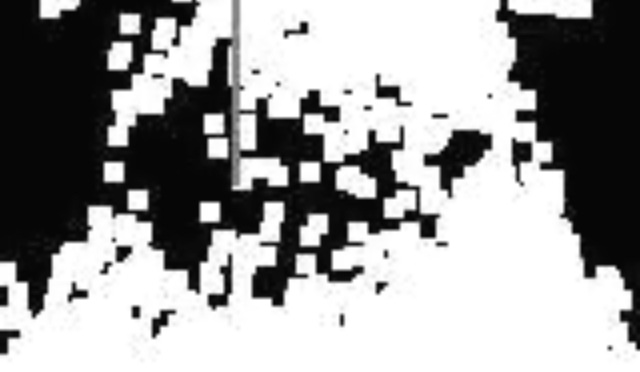
\includegraphics[width=0.27\textwidth]{pic/Tracing/erosion1.jpg}
    \label{fig:tr12}
  }
  \caption{Effect of Dilatation and Erosion}
  \label{fig:tr}
\end{figure}

\subsubsection*{Resolution}
During the actual testing process, we found that the choice of image capture resolution is also crucial. A high capture resolution can result in a high processing load on OpenMV, a low frame rate of image output, and ultimately the vehicle being unable to make timely corrections to its driving direction based on road information and potentially veering off the track. On the other hand, a low capture resolution with poor accuracy can lead to subpar performance in linear regression and unsatisfactory line tracking results. After weighing the pros and cons, we ultimately chose QQQVGA (80*60) resolution. At this resolution, even after grayscale processing and binarization, the image still yields good linear regression results, and the frame rate meets the requirement for timely correction of the vehicle's driving state.

\subsection{Approaches to Get Correct Direction}	
In this section we deal with images that have undergone basic image processing and expect to derive variables from them that can represent directions and can be understood by the machine. To do this, we explored two possible options and finally chose one of them

\subsubsection{Median of White Pixels Method with Analysis and Discussion}
The previous description mentioned that after the image undergoes binarization processing, the road portion will be highlighted in white. In this part, our main idea is to determine the direction of the turn by judging which side the white pixels lean towards in the image. This sounds very effective and does not require significant performance consumption. Additionally, the PID algorithm can be omitted during the turning process. Therefore, we initially chose this method for navigation experiments.

After a period of offline testing, we found that this method performs very well on straight roads. As long as the binarization process correctly highlights the road, the algorithm can ensure the car's stable straight-line movement. This made us very pleased. We set the Threshold to turn as shown in the Table \ref{tab:threshold}. 

\begin{table}[H]
  \centering
  \begin{tabular}{|c|c|c|c|}
    \hline
    Direction & LEFT & FORWARD & RIGHT \\
    \hline
    Meidum Value & $M<30$ & $30<M<50$ & $M>50$ \\
    \hline

  \end{tabular}
    \caption{THRESHOLD for Direction}
  \label{tab:threshold}
\end{table}

The following are the experimental results on straight road sections:

\begin{figure}[H]
  \centering
  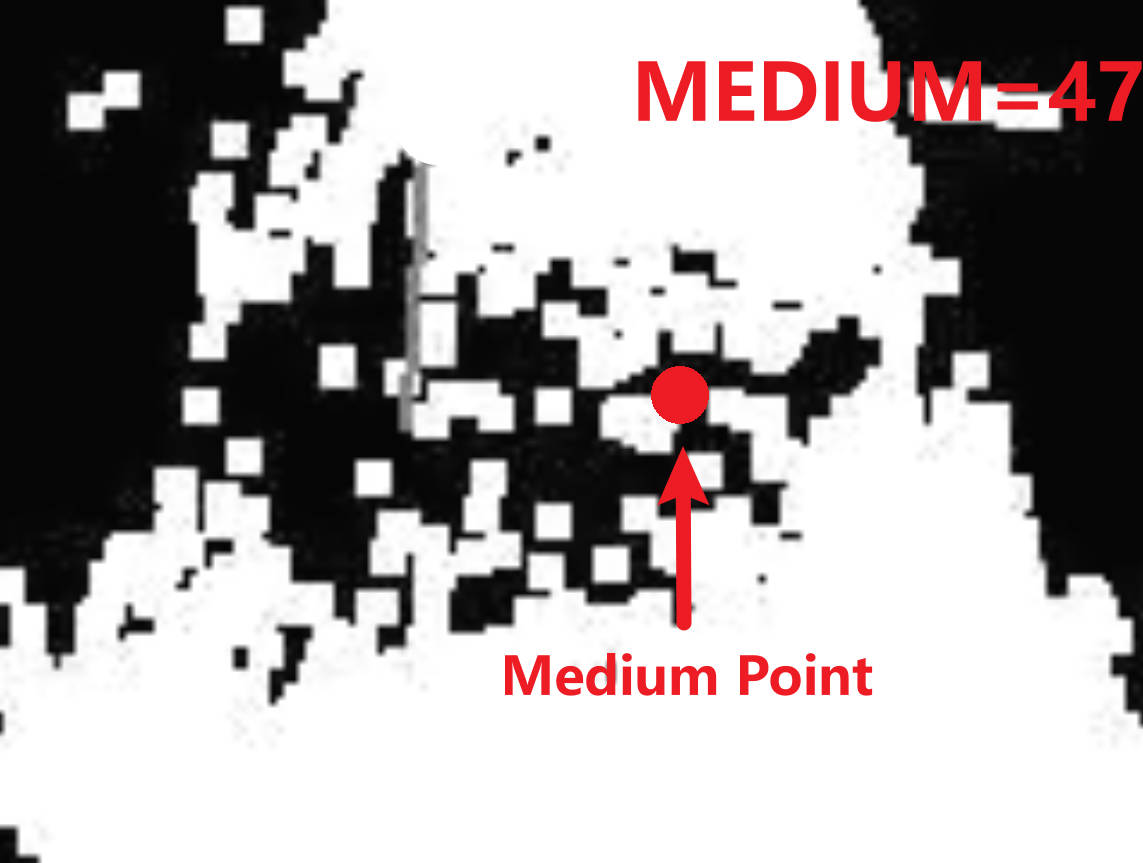
\includegraphics[width=0.35\textwidth]{pic/Tracing/Forward.jpg}
  \caption{Forward Result}
  \label{fig:example}
\end{figure}

It can be seen that the median of the white pixels obtained by the algorithm aligns well with the direction of the road. The algorithm also did not make any misjudgments on different straight road sections. To further improve the performance of the algorithm, I chose to use OpenMV's built-in algorithm to remove all small white blobs. This reduces the algorithm's load and minimizes the impact of tiny outliers.

However, we soon discovered a fatal flaw in this algorithm when using binarization as the basic image processing operation. It performs extremely unstably when a turn is required. This is because during a turn, the road needs to appear in the lower-left or lower-right of the image to correctly trigger the algorithm, as shown in the figure below:

\begin{figure}[H]
  \centering
  \subfigure[Expected right image]{
    
\includegraphics[width=0.3\textwidth]{pic/Tracing/right1.jpg}
    \label{fig:subfig1}
  }
  \hspace{0.5cm}
  \subfigure[Expected left image]{
    
\includegraphics[width=0.3\textwidth]{pic/Tracing/left1.jpg}
    \label{fig:subfig2}
  }
  \caption{Ideal turning condition}
  \label{fig:twosubfigures}
\end{figure}

However, in many cases, when making a turn, the white pixels will be evenly distributed in the lower half of the image. 

\begin{figure}[H]
  \centering
  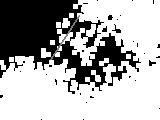
\includegraphics[width=0.3\textwidth]{pic/Tracing/wrong.jpg}
  \caption{An example for unstable condition}
  \label{fig:example}
\end{figure}

This causes the median of the white pixels' x-axis to not significantly lean towards the left or right. We considered reducing the turning threshold to improve this issue, but it would result in frequent lane departures during the straight phase. Therefore, we ultimately abandoned this approach and switched to using the linear regression method.
	\subsubsection{Linear Regression Method with Analysis and Discussion}
The linear regression algorithm is a method to obtain the "line" object after basic image processing (such as grayscale image binarization or edge detection), allowing the car to recognize the path and turn automatically like a human. First, we introduce the robust linear regression algorithm we have chosen.

The underlying algorithm of robust linear regression is based on the Theil-Sen linear regression algorithm. The basic idea of the algorithm is to calculate the slopes between all pairs of points in the data, and then select the median of these slopes as the estimated slope of the linear relationship. Then, based on the median slope, the intercept corresponding to each data point is calculated, and the median of these intercepts is selected as the estimated intercept of the linear relationship. This yields the final model of Theil-Sen regression. This algorithm has good robustness to outliers, as outliers do not have a significant impact on the final model. This is exactly what we need. Due to the complex ground conditions and inconsistent reflectivity of some sections in Patio1, the binarization processing cannot fully highlight the road, and sometimes even the gaps between bricks at the roadside are treated as white, which we define as the road, i.e., outliers, as shown in the Figure \ref{fig:linear regression}(Red arrow):



\begin{figure}[H]
  \centering
  \subfigure[Raw image]{
    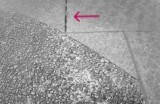
\includegraphics[width=0.33\textwidth]{pic/Tracing/turn-QQVGA.jpg}
    \label{fig:subfig1}
  }
  \subfigure[Image after binaryzation]{
    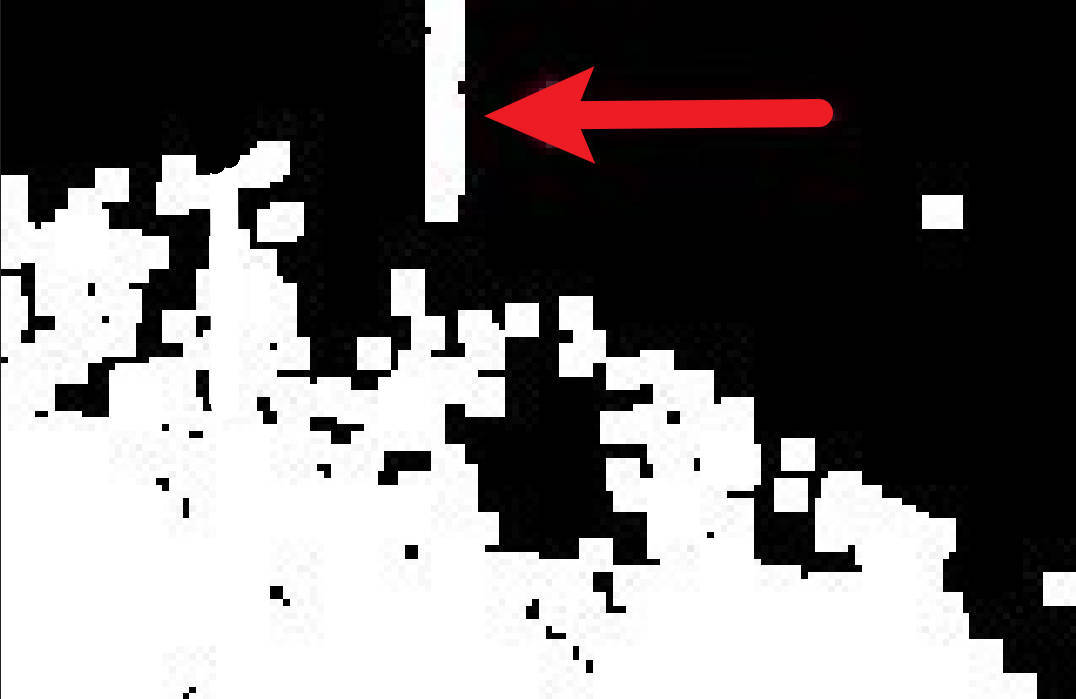
\includegraphics[width=0.33\textwidth]{pic/Tracing/turn-black-QQVGA.jpg}
    \label{fig:subfig2}
  }
  \vspace{0.5cm}
  \subfigure[Raw image]{
    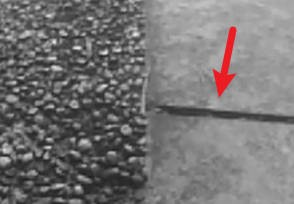
\includegraphics[width=0.33\textwidth]{pic/Tracing/outliers2.jpg}
    \label{fig:subfig3}
  }
  \subfigure[Image after binaryzation]{
    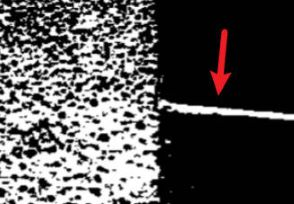
\includegraphics[width=0.33\textwidth]{pic/Tracing/outliers.jpg}
    \label{fig:subfig4}
  }
  \caption{Some examples for outlier}
  \label{fig:linear regression}
\end{figure}


The Theil-Sen linear regression algorithm can adapt well to this situation. The following is a comparison between the Theil-Sen linear regression algorithm and the fast linear regression algorithm based on least squares when significant outliers are present in Figure \ref{fig:compare} (The lines obtained by linear regression have been processed to make them more visible):


\begin{figure}[H]
  \centering
  \subfigure[Theil-Sen Regression]{
    \includegraphics[width=0.25\textwidth]{pic/Tracing/Robust.jpg}
    \label{fig:compare1}
  }
  \hspace{0.5cm}
  \subfigure[Least Square Method]{
    \includegraphics[width=0.25\textwidth]{pic/Tracing/Fast.jpg}
    \label{fig:compare2}
  }
  \caption{Comparison between two possible methods}
  \label{fig:compare}
\end{figure}


It can be seen that the estimation of the fast linear regression is completely wrong, while Theil-Sen linear regression produces more desirable results, which is turn left. However, implementing Theil-Sen linear regression algorithm is a challenging task. Fortunately, OpenMV provides a powerful library function,

\begin{lstlisting}[language=Python]
line = Image.get_regression()

\end{lstlisting}


We only need to set the "Robust" parameter to True to call the Theil-Sen linear regression. Based on this library function, I have encapsulated a Tracing function:

\begin{lstlisting}[language=Python]
import image

def Tracing(Image,threshold,bool,ROI):
    if bool:
        Image.erode(2)
    Image.dilate(2)
    line = Image.get_regression([threshold], invert=False, robust=True, roi=ROI)
    if (line): Image.draw_line(line.line(), color = 127, thickness=2)
    return line

\end{lstlisting}


which includes the image processing steps mentioned above, making it convenient for debugging in the main program and allowing the main program to focus on logic implementation.

Through the Theil-Sen linear regression algorithm, we successfully obtain the "line" object that can accurately represent the direction under most road conditions. On the OpenMV platform, this line is described using polar coordinates, which means that the line can be described using the polar radius $\rho$ and the angle $\theta$, as shown in Figure \ref{fig:line}. 

\begin{figure}[H]
  \centering
  \includegraphics[width=0.8\textwidth]{pic/Tracing/Line.jpg}
  \caption{An example for line description \cite{AGYEMAN_2017}}
  \label{fig:line}
\end{figure}

These two important parameters can be implemented using methods specific to the line object, shown below:


\begin{lstlisting}[language=Python]
Polar_radius = Line.rho()
Angle = Line.theta()
\end{lstlisting}



These two values will be transmitted to STM32 for further processing via inter-board communication and finally used as parameters for the PID algorithm to control the car.
\subsection{Results}
After employing the aforementioned image processing methods, we achieved acceptable results in Patio1. The following Table \ref{tab:re} presents the statistical summary of anomalies encountered during 10 attempts.

\begin{table}[H]
    \centering
    \begin{tabular}{|c|c|c|c|c|c|c|c|c|c|c|c|c|}
    \hline
        \multicolumn{11}{|c|}{\textbf{Error Counting}} & \multirow{2}{*}{\textbf{Total Error}} \\ \cline{1-11}
        \textbf{Experiment Index} & 1 & 2 & 3 & 4 & 5 & 6 & 7 & 8 & 9 & 10 &\\ \hline
        \textbf{1st Straight Section} & 1 & 0 & 0 & 1 & 0 & 0 & 0 & 0 & 0 & 0 &2\\ \hline
        \textbf{1st turn} & 1 & 1 & 0 & 0 & 0 & 0 & 0 & 0 & 0 & 0 &2\\ \hline
        \textbf{2nd Straight Section} & 1 & 0 & 0 & 0 & 0 & 2 & 0 & 0 & 0 & 1 &4\\ \hline
        \textbf{2nd Turn} & 0 & 0 & 0 & 0 & 0 & 0 & 0 & 0 & 0 & 0 &0\\ \hline
        \textbf{3th Straight Section} & 0 & 0 & 0 & 0 & 0 & 0 & 0 & 0 & 0 & 0 &0\\ \hline
        \textbf{3th Turn} & 0 & 1 & 0 & 0 & 0 & 0 & 0 & 0 & 0 & 0 &1\\ \hline
        \textbf{4th Straight Section} & 1 & 0 & 0 & 0 & 0 & 0 & 0 & 0 & 0 & 0 &1\\ \hline
        \textbf{4th Turn} & 0 & 0 & 0 & 0 & 0 & 0 & 0 & 0 & 0 & 0 &0\\ \hline
        \textbf{5th Straight Section} & 0 & 0 & 0 & 0 & 0 & 0 & 0 & 0 & 0 & 0 &0\\ \hline
    \end{tabular}
    \caption{Results of Attemption of Tracing Module}
    \label{tab:re}
\end{table}
The above results come from tests after the track was disrupted. Due to problems with the chosen technical route, our image tracing module was significantly less effective on the affected sections, and it is evident that the number of times the trolley deviated from its route before the second turn was relatively high.

The choice of edge recognition may be feasible if the impact of road damage is to be addressed. However, due to time constraints, we were not able to switch technical paths in the two days available, which can be improved in the future

\subsection{Conclusions and Future Works}
During the process of completing the entire subsystem, I encountered numerous challenges and gained a wealth of knowledge. Eventually, I delivered this mature module to the team. In the initial design phase, we explored various potential solution paths, which was of paramount importance. These attempts laid a solid foundation for achieving more optimal solutions and significantly broadened my perspective. Subsequently, I conducted offline field tests. In the initial tests, algorithms that I expected to perform exceptionally well did not meet my expectations. This made me realize that solutions developed in the laboratory may not always adapt well to real-world scenarios. As a result, I insisted on on-site development and immediate testing strategies during the subsequent debugging process, which saved me a considerable amount of time. Additionally, through communication with other team members, I discovered that some groups adopted highly complex algorithms that exhibited unstable performance. This indicates that complexity does not necessarily equate to excellent performance. To achieve good results, it is necessary to combine practical considerations and choose the most universally applicable methods for implementation.

Regarding future work, I believe that my visual line-tracing system lacks stability under different weather conditions. After conducting some research, I attribute this issue primarily to the fixed black and white threshold values, which cannot adaptively adjust. However, achieving this adaptive threshold effect is not impossible. I will attempt to implement an algorithm for adaptive thresholding and anticipate that it will result in more stable performance.

\subsection{Acknowledgements to My Friend}
Lastly, I would like to express my gratitude to my team member and roommate, Si Yuan. Throughout the 12-day period of offline development and testing, he accompanied me to the field every day, enduring the scorching summer heat, and assisted me in recording experimental data and organizing materials. Without him, I would not have been able to successfully complete the development of the line-tracing system or maintain my pursuit of excellent performance. He has been an essential source of emotional support and has provided invaluable assistance to my work that cannot be measured in monetary terms.

\newpage
\section{Pitching Function of OpenMV}\label{sec:Pitch}
\colorbox{yellow}{\textbf{Developer:} Bi Bodong 2613939B}
	
\subsection{Pitching Module}

In the early stage of visual system design, we aimed to enable OpenMV to achieve programmable angle adjustment, which would facilitate later line-following debugging. In addition, since arrow recognition in Patio2 requires a camera perspective different from that of the line-tracing task, a programmable pitch adjustment system would allow us to quickly switch camera perspectives during offline testing.

\subsection{Realization of Pitching Module}
The pitch adjustment system is implemented using programmable servos, as shown in the figure below:

\begin{figure}[H]
  \centering
  \includegraphics[width=0.4\textwidth]{pic/servo.png}
  \caption{Programmable Servo}
  \label{fig:servo-1}
\end{figure}

 It can be observed that the servo gimbal has two adjustable angles, and according to the parameter manual, the range of these two angles is 0-180 degrees.
 
 \subsubsection*{Power Supply}
In order to power the servo, we require an external 5V battery. This external battery is connected to the servo using a 2-pin connector. Surprisingly, this external battery can also provide power to the OpenMV simultaneously. As shown in the above diagram, the connection between the servo and OpenMV is straightforward, where the pins on the OpenMV board can be inserted into the corresponding pin sockets on the servo.

 \subsubsection*{Servo Program}
To initialize the servo, we need to program it, which is relatively simple using the built-in Python compiler in OpenMV. The pins of OpenMV will control the motor's rotation angle by outputting PWM signals. Therefore, we only need to set the minimum and maximum input values to control the servo's rotation to the desired angle. The following code shows how we get 180 degree:

\begin{lstlisting}[language=Python]
from pyb import Servo

# Create servo object to control the servo
s1 = Servo(1) # P7-upper servo
s2 = Servo(2) # P8-lower servo

s1.calibration(500,2500,500)
s2.calibration(500,2500,500)

s1.pulse_width(2500)
s2.pulse_width(2500)	
\end{lstlisting}

 \subsubsection*{Reliability Analysis}
 Due to cost constraints, we opted not to purchase servo gimbals equipped with servo motors and instead chose a cheaper version that utilizes stepper motors. However, one major drawback of stepper motors is their lack of precision. In order to assess whether such inaccuracies would affect the camera's performance, a reliability analysis of the servo was conducted using the following methodology:
  \begin{enumerate}

\item \textbf{Outputting a fixed pulse width PWM wave to the servo}
\item \textbf{Use the angle meter to measure the angle of rotation of the servo}
\item \textbf{Calculate the error between the expected rotation angle and the actual rotation angle}
\item \textbf{Calculate the average value of the angular error}
\end{enumerate}
The experimental results are presented as follows:


\begin{table}[H]
    \centering
\begin{tabular}{|*{12}{c|}}

  \hline
  Number of Experiments & 1 & 2 & 3 & 4 & 5 & 5 & 7 & 8 & 9 & 10 & Average Error (Degree)\\
  \hline
  Angle Error (Degree)& 6 & 14 & 3 & 0 & 1 & 11 & 5 & 3 & 17 & 2 &6.2\\
  \hline
  
\end{tabular}
    \caption{Angle Error}
    \label{tab:reliability}
\end{table}

It can be observed that there is a relatively large error in the stepper motor gimbal. The target angle we have chosen is 90 degrees, resulting in an error rate of: 
$$R_{error}=\frac{\text{Average Angle Error}}{\text{Target Angle}}\times 100=\frac{6.2}{90}\times 100=6.8\text{\%}$$
During the initial construction of the vision module, we are unable to assess whether this error will have an impact on line following or arrow recognition. However, this error is no longer negligible. So, in the final integrated debugging of the entire vehicle, the application of this module needs to be carefully considered.

\newpage
\section{Arrow Identification}\label{sec:Arrow}
\colorbox{yellow}{\textbf{Developer:} Ruan Haoxi 2613909R}

\subsection{Task Analysis}
In this part, OpenMV is used to realize the task of arrow identification and send different messages to stm32 according to the heading of the arrow, so that the rover can move to the right direction.
\subsection{Method Analysis}
\subsubsection{Initial Method: Neural Network (Not Applied)}
The platform we choose to achieve the vision task is OpenMV. Because OpenMV supports the Python language and can import the TensorFlow Lite package for machine vision processing, I initially planned to use a neural network to implement an arrow recognition task. That is because using a neural network for visual tasks offers several advantages. For instance, neural networks have the ability to learn and extract complex features from images, enabling them to identify patterns and objects with high accuracy. However, I found neural network may not be the best method to handle arrow identification, because training a neural network requires a large amount of data as a training set. Unfortunately, I did not find a training set which only contains arrows on the internet. Second, neural network is more suitable to handle more difficult vision tasks, for example, identifying a several classes of objects, but not three arrows with different directions. To overcome these limitations, an alternative approach that can be considered is template matching. 
\subsubsection{Final Method: Template Matching Based on OpenMV (Adopted) }
Template matching is a computer vision technique used to locate specific patterns or objects within an image. Template matching involves comparing an input image with a predefined template or pattern to identify matches. In the case of arrow recognition, a template of an arrow shape can be saved in OpenMV in advance , and the image can be searched for similar patterns. It involves comparing a small reference image, known as a template, with the target image. Template matching has many advantages, for instance. It is a simpler and more straightforward approach compared to neural networks, as it does not require extensive training or complex model architectures. Furthermore, template matching is computationally efficient and can be easily implemented on resource-constrained devices like OpenMV cameras. The algorithm is typically lightweight and can run in real-time without significant processing overhead. Moreover, template matching provides interpretability as the matching process is based on direct pixel comparisons between the template and the image. This transparency allows for better understanding and control over the recognition process. 
\subsection{Method Implementation}
Firstly, The pictures of three arrows of with different directions were saved in OpenMV in advance. These three pictures will be the templates of the arrows. 

\begin{figure}[H]
  \centering
  \includegraphics[width=0.5\textwidth]{pic/Arrow Rec/1.png}
  \caption{The pictures of three arrows}
  \label{fig:The pictures of three arrows}
\end{figure}

\begin{lstlisting}[language=Python]
template0 = image.Image("/ahead.pgm")
template1 = image.Image("/right.pgm")
template2 = image.Image("/left.pgm")
a = Image.find_template(template0, 0.70, step=4, search=SEARCH_EX)
r = Image.find_template(template1, 0.80, step=4, search=SEARCH_EX)
l = Image.find_template(template2, 0.80, step=4, search=SEARCH_EX)
\end{lstlisting}
This code is in the Matching function, "/ahead.pgm", "/right.pgm"and "/left.pgm" referred to the pictures of the three arrows, they were saved in OpenMV in advance. The first three rows of code defined them as template0, template1 and template2. "Image.find\_template" is a function used to call out Template matching, it allows OpenMV to compare the images captured by the camera with the  save templates, and match them automatically. a, r and l represent three situations which state ahead, right or left arrow is identified successfully.
\begin{lstlisting}[language=Python]
if a:
    Image.draw_rectangle(a)
    return 0
elif r:
    Image.draw_rectangle(r)
    return 1
elif l:
    Image.draw_rectangle(l)
    return 2
\end{lstlisting}
In this code, I used a if statement to set three conditions. In the first condition, the forward arrow is identified, the function returns 0. In the second condition, the right arrow is identified, the function returns 1. In the third condition, the left arrow is identified, the function returns 3.
\begin{lstlisting}[language=Python]
    if T == 0:
        pinl.high()
        pinr.low()
        time.sleep(0.5)
    elif T == 1:
        pinl.low()
        pinr.high()
        time.sleep(0.5)
    elif T == 2:
        pinl.high()
        pinr.high()
        time.sleep(0.5)
\end{lstlisting}
This code is in the main function, which can call the Matching function and send signals to stm32 using the pins on OpenMV and make the rover turn to different directions. Pinl controls P2 on OpenMV, pinr controls P3 on OpenMV. In the first condition, T=0, that means a forward arrow is identified, pinl has a high level output and pinr has a low level output. In the second condition, T=1, that means a right arrow is identified, pinl has a low level output and pinr has a high level output. In the third condition, T=2, that means a right arrow is identified, both pinr and pinl have a high level output. time.sleep(0.5) is used to make sure that the signal will last for 0.5s, in case that the change of output is too short which cause stm32 can not receive it.
    \subsection{Reliability Analysis}
In order to test the accuracy of template matching method, several experiments are conducted. In each experiments, the three arrows with different directions were placed in front of the camera of OpenMV with a distance range of 15-20 centimeters for 10 times and the outputs of the OpenMV were recorded at the same time. In this experiment, I add a “print” in the code temporarily, which makes it easier to judge whether the arrow is identified correctly. If the forward arrow is identified, the console of the OpenMV IDE print F, if the right arrow is identified, it prints R and for a left arrow, it prints L. The result is listed in the table below.

\begin{table}[H]
    \centering
\begin{tabular}{|*{12}{c|}}

    \hline
  Experiment Index & 1 & 2 & 3 & 4 & 5 & 6 & 7 & 8 & 9 & 10 & Accuracy\\
    \hline
  Forward & F & F & F & F & F & F & F & F & F & F & 100\text{\%}\\
    \hline
  Right & R & L & L & L & R & R & R & R & L & R & 60\text{\%}\\
    \hline
  Left & R & R & L & R & L & L & R & R & L & L & 50\text{\%}\\
    \hline
  
\end{tabular}
    \caption{Result of the first experiment}
    \label{tab:Result of the first experiment}
\end{table}

It can be seen obviously that the accuracy of identifying forward arrow is very high, which is 100\text{\%}, But for left and right arrow the accuracy is very low. From the table I have noticed that left and right arrows were often confused in the identification.
\subsubsection{Problem analysis}
The problem in template matching was that the right and left arrow were often confused in the identification. After analyzing this problem with the knowledge of  the principle of template matching , I believe that the confusion between left and right arrows is due to their templates have high similarity, because the “long bar” of these two arrows take up much space. The fact that the forward arrow can be identified correctly with 100\text{\%} also supports this hypothesis.

\begin{figure}[H]
  \centering
  \includegraphics[width=0.4\textwidth]{pic/Arrow Rec/4.png}
  \caption{High similarity of right and left arrow}
  \label{fig:High similarity of right and left arrow}
\end{figure}

\subsubsection{Solution of the Problem}
The cause of the problem is that the templates of right and left arrow have a high similarity. It can be easily thought that the solution is to reduce the similarity of the templates of right and left arrow. To be more specific, the similar part of the templates should be cut off and only retain the different part. So I chose to cut off the “long bar” of the templates of right and left arrow ad=nd only retain the head of the arrow.

\begin{figure}[H]
  \centering
  \includegraphics[width=0.9\textwidth]{pic/Arrow Rec/5.png}
  \caption{The optimized templates of right and left arrow}
  \label{fig:The optimized templates of right and left arrow}
\end{figure}

\subsubsection{Accuracy Test After Optimization}
After changing the templates of right and left arrows to make them be more different with each other. I carried out the same experiment with the first time to test the accuracy of identification.

\begin{table}[H]
    \centering
\begin{tabular}{|*{12}{c|}}

    \hline
  Experiment Index & 1 & 2 & 3 & 4 & 5 & 6 & 7 & 8 & 9 & 10 & Accuracy\\
    \hline
  Forward & F & F & F & F & F & F & F & F & F & F & 100\text{\%}\\
    \hline
  Right & R & R & R & R & R & R & R & R & L & R & 90\text{\%}\\
    \hline
  Left & L & L & L & L & L & L & L & L & L & L & 100\text{\%}\\
    \hline
  
\end{tabular}
    \caption{Result of the second experiment}
    \label{tab:Result of the second experiment}
\end{table}

It can be seen that the accuracy of identifying right and left arrows increase significantly and the accuracy of identifying forward arrow still remains high. The problem was solved successfully and template matching had a high reliability now.

\subsection{Task of Arrow Identification}
In this task, the rover will identify the arrow placed at point A using vision module: Arrow identification based on OpenMV. At the beginning, the rover will go to point A along the direction of the red arrow, when it will stop before the arrow and keep a distance of 10-20 centimeters from it. At this time, the vision module will be activated and start identifying the arrow. There are totally three conditions. 

\begin{figure}[H]
  \centering
  \includegraphics[width=0.5\textwidth]{pic/Arrow Rec/7.jpg}
  \caption{Sketch map of the task}
  \label{fig:Sketch map of the task}
\end{figure}

1. The arrow at point A is a left arrow, the rover should turn 135 degrees to left and go straight ahead for a distance, then knock the bottle placed at point B. Finally, the rover turn right and go to area E to process the next task.

2. The arrow at point A is a forward arrow, the rover should turn 90 degrees to left and go straight ahead for a distance, then knock the bottle placed at point C. Finally, the rover turn right and go to area E to process the next task.

3. The arrow at point A is a forward arrow, the rover should turn 45 degrees to left and go straight ahead for a distance, then knock the bottle placed at point C. Finally, the rover turn right and go to area E to process the next task.

\newpage
\section{Ultrasonic Distance Detection}\label{sec:SR-04}
\colorbox{yellow}{\textbf{Developer:} Zhang Ziao 2613934Z}

\subsection{HC-SR04}
	
The ultrasonic detection is applied during the project for beacon detection and distance measuring, and the ultrasonic module which is used in the project is HC-SR04. 
	
HC-SR04 is an ultrasonic detecting sensor, and it could be assembled with the Nucleo Development Board, which shapes like Figure \ref{fig:HC-SR04}. The HC-SR04 sensor consists of a transmitter and a receiver. The transmitter emits an ultrasonic pulse, which encounters an obstacle and gets reflected back to the receiver. By measuring the round-trip time of the signal, the HC-SR04 can calculate the distance between the sensor and the object.

This sensor offers several advantages. Firstly, the HC-SR04 provides high accuracy and rapid response, delivering precise measurements in very short time frames. Secondly, it has a relatively large measurement range, typically able to measure distances between 2 centimeters and 400 centimeters according to Figure \ref{fig:Specifications of HC-SR04}. Additionally, the HC-SR04 sensor is known for its low power consumption and straightforward usage, requiring only a few pins and basic circuit connections to enable distance measurement functionality.

However, there are some limitations to consider with the HC-SR04 sensor. Firstly, it may exhibit measurement errors for specific types of objects or in certain environments. For instance, absorbing materials or irregular surfaces can lead to inaccurate distance measurements due to the reflection of ultrasonic waves.

In summary, the HC-SR04 ultrasonic sensor is a powerful and extensively utilized distance measuring sensor. Its features of high precision, rapid response, and ease of use make it an ideal choice for our rover.
\begin{figure}[H]
  \centering
  \includegraphics[width=0.5\textwidth]{pic/HC-SR04/HC-SR04.png}
  \caption{Image of HC-SR04}
  \label{fig:HC-SR04}
\end{figure}
\begin{figure}[H]
  \centering
  \includegraphics[width=0.5\textwidth]{pic/HC-SR04/Specifications of HC-SR04.png}
  \caption{Specifications of HC-SR04}
  \label{fig:Specifications of HC-SR04}
\end{figure}

The the functions of the pins on HC-SR04 and the measuring process of the HC-SR04 can be summarized as follows.

There are 4 pinouts in the HC-SR04 shown in the Figure \ref{fig:HC-SR04}, which are the VCC pin(1), the Trig pin(2), the Echo pin(3) and the GND pin(4). 
\begin{itemize}

\item \textbf{VCC}: connected to the 5V pin on the Nucelo development board to drive HC-SR04. 
\item \textbf{Trig}: used to trigger the ultrasonic pulse. 
\item \textbf{Echo}: Output high level after the ultrasonic waves are sent until the reflected waves are received.
\item \textbf{GND}: connected to ground on the Nucelo development board.
\end{itemize}
To start measuring, a trigger signal is sent to the sensor by applying a high-level pulse of at least 10 microseconds to the trigger pin. Upon receiving the trigger signal, the HC-SR04 activates its transmitter, which converts the electrical signal into a 40 kHz ultrasonic pulse. This emitted pulse propagates through the air in a cone-shaped pattern until it encounters an object or obstacle in its path.

When the ultrasonic pulse reaches an object, it gets reflected back towards the sensor. The HC-SR04's receiver, upon detecting the reflected pulse within a specified time frame, generates an output pulse. The duration of this output pulse corresponds to the time taken for the ultrasonic pulse to travel to the object and back.

By measuring the duration of the pulse, the HC-SR04 sensor can calculate the distance between itself and the object based on the known speed of sound. This calculation involves multiplying the pulse duration by the speed of sound and dividing it by two, as the ultrasonic pulse travels to the object and back.

Overall, through the timing of the emitted and received pulses, the HC-SR04 ultrasonic distance sensor provides an effective means of distance measurement.

\subsection{Application}
\subsubsection{Ultrasonic Sensor Layout}
Three ultrasonic sensors are mounted on the lower layer of the rover. As shown in Figure 3.49, Figure 3.50, and Figure 3.51, we placed one ultrasonic sensor on the front side of the rover, one on the left side, and two on the right side. The ultrasonic sensors are fixed on brackets, which are adhesive-bonded to the lower layer. The height of the ultrasonic sensors is carefully designed to avoid the hollow sections of the railing around the lake in Patio2, ensuring that the sensors can continuously receive distance signals from the ultrasonic waves as the rover moves.
\begin{figure}[H]
  \centering
  \includegraphics[width=0.7\textwidth]{pic/HC-SR04/front view.jpg}
  \caption{Front View of Sensor Layout}
  \label{fig:Front View of Sensor Layout}
\end{figure}
\begin{figure}[H]
  \centering
  \includegraphics[width=0.7\textwidth]{pic/HC-SR04/left view.jpg}
  \caption{Left View of Sensor Layout}
  \label{fig:Left View of Sensor Layout}
\end{figure}
\begin{figure}[H]
  \centering
  \includegraphics[width=0.7\textwidth]{pic/HC-SR04/right view.jpg}
  \caption{Right View of Sensor Layout}
  \label{fig:Right View of Sensor Layout}
\end{figure}

\newpage
\section{Message Wireless Transmission}\label{sec:hc12}
\colorbox{yellow}{\textbf{Developer:} Li Zhengjie 2614370L}

\subsection{Task Requirements}
In the patio 2, there is a square area where the wireless communication happens. When the rover reaches at this designated location, the task of sending the message which contains the team member list and real-time information from the microcontroller on the mechanical trolley to the PC terminal. This wireless communication will be achieved by utilizing HC-12 module for the function of serial communication. The used devices, relevant technical details and principles are introduced briefly in the following content.  





\subsection{HC-12 Module}
HC-12 is a wireless transceiver module commonly used for long-range wireless communication in embedded systems. It provides a simple and convenient way to establish wireless serial communication between microcontrollers or other devices. It supports half-duplex communication and uses a simple AT command set to configure its parameters, such as the frequency, baud rate, and transmission power. It operates in a transparent mode, which means it can be used to replace wired serial communication without modifying the existing code or protocol. In addition, the HC-12 module offers a serial interface, allowing it to be easily connected to microcontrollers. The HC-12 module communicates via radio waves and it uses FSK modulation technology (Frequency Shift Keying Modulation). The following is the basic principle of communication between two HC-12 modules via radio waves.The operating frequency of both HC-12 modules needs to be set to ensure they communicate on the same frequency. HC-12 modules support a range of configurable operating frequencies, such as 433MHz, 868MHz or 915MHz. The operating frequency is set via the AT command (e.g. AT+Cxxx), where xxx is the parameter for the frequency. The data to be sent is sent to an HC-12 module via a serial interface (e.g. UART). the HC-12 module encodes and modulates the data and then converts it to radio waves. The HC-12 module in transmit mode sends the modulated signal as a radio wave. The radio waves travel through the air at a specific frequency and are sent out through an antenna.The HC-12 module in receive mode receives the radio waves in transmit mode through the antenna. Then, it demodulates and decodes the received signal to restore the original data signal. The decoded data is output to the connected devices through the serial port interface. The device can receive the information sent from another HC-12 module by reading the data in the serial port buffer. 

According to the datasheet, the HC-12 module has four serial port transparent transmission modes which are respectively FU1, FU2, FU3, and FU4.The FU1 and FU2 are both power-saving modes which sacrificing the communication distance. While the FU4 is the ultra-long distance communication mode, it could only transmit small amount of data.The FU3 mode balances the communication distance and the amount of the transmitted data.The HC-12 module has channels CH001 to CH127.The default value of wireless channel is 001 and the operating frequency is 433.4MHz. The channel step is 400KHz and the operating frequency of channel 100 is 473.0MHz. The modules always realize the function of wireless transmission in pairs, with data transmitted by means of a half-duplex link. On the purpose of transmitting the message successfully, the transmission mode,baud rate, and wireless communication channel of the two HC-12 modules must stay the same. The factory default module settings are: FU3, 9,600bps (8N1: 8 data bits, no parity, 1 stop bit), CH001 (433.4MHz), 20dBm power (100mW) which are the Figure shows the HC-12 wireless module and matched test stand.

\begin{figure}[H]
  \centering
  \subfigure[HC-USB-T Test Stand]{
    \includegraphics[width=0.4\textwidth]{pic/HC12/hc12-4.png}
    \label{fig:hc12-4}
  }
  \hspace{0.5cm}
  \subfigure[HC-12 Wireless Module]{
    \includegraphics[width=0.4\textwidth]{pic/HC12/hc12-5.png}
    \label{fig:hc12-5}
  }
  \caption{The whole module of the HC-12}
  \label{fig:hc12-4-5}
\end{figure}
The Figure shows the module size of the module:
\begin{figure}[H]
  \centering
  \includegraphics[width=0.4\textwidth]{pic/HC12/hc12-6.png}
  \caption{Module Size}
  \label{fig:hc12-6}
\end{figure}

The streamlined instruction table for key pin: 
\begin{table}[H]
\caption{Pin Definition}
\begin{tabular}{|c|c|c|c|}
\hline
Pin & Definition & I/O & Instruction \\
\hline
1 & VCC & None & Power input, DC3.2V-5.5V, 200mA. \\
\hline
2 & GND & None & Common ground \\
\hline
3 & RXD & Input & URAT input port \\
\hline
4 & TXD & Output & URAT output port \\
\hline
5 & SET & Input & Parameter setting control pin,   effective at low level \\
\hline
6 & ANT & RF Input/Output & 433MHz antenna pin \\
\hline

\end{tabular}
\end{table}

	\subsection{Design Details}
	Initially, it is expected to utilize microcontroller mbed carrying the trickle-charge timekeeping chip DS1302 to realize the acquisition of the real time.The timekeeping chip uses simple serial port to communicate with mbed and mbed utilizes the UART serial communication by HC-12 module to send time information to the PC terminal. However, the pins of the mbed are almost used to support the master control program and the additional wires could make the space in the middle of the car extremely compressed. The method of configuring the real time clock module(RTC) in OpenMV directly is finally chosen to acquire the time information.The time library and pyb library are import to the program to configure RTC and construct the wireless communication channel. After initialing the RTC module as the code shows, the time information of year, month, day, hour, minute and second is sent to PC terminal.
	
	\begin{lstlisting}[language=Python]
Time = (2023, 6, 3, 6, 1, 0, 0, 0)
\end{lstlisting}

In order to make the rover do not send the required message until it reaches at the designated region, an input from the mbed is considered as a switch to control the wireless transmission. When the rover arrives at the designated location, a signal will be generated and sent to OpenMV. As soon as the computer receives the input signal, the transmission will start and send the message after the every interval of one second. The input signal will disappear once the wall could not be detected by ultrasonic sensor so that this transmission process will end after the rover drives out of the designated area.

\begin{lstlisting}[language=Python]
import time
from pyb import RTC
from pyb import UART

uart = UART(3, 9600)

rtc = RTC()

def Transmit(IF_Trans, Time):
    rtc.datetime(Time)
    while (IF_Trans==1):
        current_time = rtc.datetime()
        name = (("Messages: Here we sent the member's name"))
        time_string = "{}/{}/{} {}:{}:{}\n{}".format(current_time[0], current_time[1], current_time[2], current_time[4], current_time[5], current_time[6], name)
        time.sleep_ms(1000)
        uart.write(time_string + '\n')
\end{lstlisting}

	\subsection{Wiring Link}
	One HC-12 module is connected to the OpenMV. The Pin 6 of OpenMV is considered as the switch to give a signal to control the start and end of the transmission. The  Pin 4 is the RX of OpenMV which should be connected to the TX of HC-12 module. The Pin 5 is the TX of OpenMV which should be connected to the RX of HC-12 module. The HC-12 module should also be connected to the Ground and VCC. Another HC-12 module is directly connected to the PC terminal by the HC-USB-T test stand. 
	
	\begin{figure}[H]
  \centering
  \subfigure[Rover Terminal]{
    \includegraphics[width=0.4\textwidth]{pic/HC12/hc12-7.png}
    \label{fig:hc12-4}
  }
  \hspace{0.5cm}
  \subfigure[PC Terminal]{
    \includegraphics[width=0.4\textwidth]{pic/HC12/hc12-8.png}
    \label{fig:hc12-5}
  }
  \caption{Two Terminal Connection}
  \label{fig:hc12-7-8}
\end{figure}

The Serial Debug Assistant shown as Figure is the window to present the received information. After the HC-12 module is connected to the PC terminal, the correct serial port should be chosen.  

\begin{figure}[H]
  \centering
  \includegraphics[width=0.8\textwidth]{pic/HC12/hc12-9.png}
  \caption{Chosen PC Port Tool}
  \label{fig:hc12-9}
\end{figure}

\subsection{Results}
With the python program inserted to the OpenMV, the wireless charging between rover and laptop is realized. After the rover reaches at the designated region, the required message is sent to the PC by HC-12 module repeatedly once a second. The required task of wireless communication is accomplished as the Figure shows.

\begin{figure}[H]
  \centering
  \includegraphics[width=0.85\textwidth]{pic/HC12/hc12-10.png}
  \caption{Result}
  \label{fig:hc12-10}
\end{figure}

The rover successfully transmits the message contains time information, team number and the name list of group members. Sometimes it will receive unexpected message since several groups transmit the message simultaneously can lead to incorrect reception of information. This problem could be solved by change the baud or the working wireless channel since most teams directly use the default settings like 9600 baud and CH001. If the settings are differ from those of other teams, the HC-12 module would not receive unexpected message. One thing to pay attention to is delay due to data processing and transmission which makes major contribution to a few seconds of error, however, it seldom happens. 

\newpage
\section{Table Tennis Ball Release Module}\label{sec:tb}
\colorbox{yellow}{\textbf{Developer:} Zheng Jiashu 2614397L}

\subsection{Initial Design}
Figure \ref{fig:tb1} shows the initial design for the table tennis ball release module.

\begin{figure}[H]
  \centering
  \includegraphics[width=0.7\textwidth]{pic/Table tennis/9.png}
  \caption{The Model for Initial Design}
  \label{fig:tb1}
\end{figure}

However, I improved the design of ball slot in my final design as shown in figure \ref{fig:tb2} considering the stability of this device through many fieldworks and trials. Firstly, the length of the slot extended to prevent the ping pong ball from slipping easily due to the shaking of the rover during operation. Secondly, the shape of the ball slot has been changed to a near complete cylinder to better enclose the table tennis ball, shielding it from the surrounding wind and improving the stability and hit rate of the module.

\begin{figure}[H]
  \centering
  \includegraphics[width=0.85\textwidth]{pic/Table tennis/10.png}
  \caption{The Model for Final Design}
  \label{fig:tb2}
\end{figure}

Figure \ref{fig:tb3} shows the finished product according to the final design which made by wooden boards, plastic water bottle and other materials.

\begin{figure}[H]
  \centering
  \includegraphics[width=0.7\textwidth]{pic/Table tennis/11.jpg}
  \caption{Actual Device}
  \label{fig:tb3}
\end{figure}

\subsection{Structure}

\begin{figure}[H]
  \centering
  \includegraphics[width=0.85\textwidth]{pic/Table tennis/12.png}
  \caption{The Structure of The Device}
  \label{fig:tb4}
\end{figure}

As shown in figure \ref{fig:tb4}, it consists of a slope with angle $\alpha$, a small electric fan on the base and a ball slot. The electric fan is made of a motor and a matching blade. The small angle $\alpha$ ensures that the ball does not fall during normal operation while it allows the ball to be blown out of the slot by the wind. The base raises the height of the motor to prevent the fan blades from contacting the slope when rotating. Table tennis ball is placed in the slot before beginning task1 in patio2.  

\subsection{Connection}

\begin{figure}[H]
  \centering
  \includegraphics[width=1\textwidth]{pic/Table tennis/13.png}
  \caption{The Connection Between the Device and The Components of The Rover}
  \label{fig:tb5}
\end{figure}

As shown in Figure \ref{fig:tb5}, two pins of the motor are connected to two output pins of the motor drive. For this motor drive, the three input pins are connected to three DigitalOut pins of MCU. Additionally, 5V output of MCU is used to power and activate the motor drive. Finally, all of three GND pins of the motor drive are connected with the ground of MCU together.

\subsection{Control Method}

According to the control logic of the motor drive and Figure \ref{fig:tb5}, it is obvious that this fan can be controlled by setting output of three DigitalOut pins of STM32.

\begin{table}[H]
    \centering
    \begin{tabular}{|l|l|l|l|}
    \hline
        Mode & DigitalOut1 & DigitalOut2 & DigitalOut3 \\ \hline
        Inward Suction  & 1 & 0 & 1 \\ \hline
        Outward Blowing  & 1 & 1 & 0 \\ \hline
    \end{tabular}
    \caption{Logic For Two Modes}
    \label{tab:tb1}
\end{table}

Table \ref{tab:tb1} shows the method to controlling the device work in two different modes. For inward suction mode, the fan would blow air inward to inhale the ping-pong ball as shown in Figure \ref{fig:tb6}(a), while for outward blowing mode shown in Figure \ref{fig:tb6}(b), the fan would blow air outward to push the ping-pong ball away from the ball slot and into the basket.

\begin{figure}[H]
  \centering
  \includegraphics[width=1\textwidth]{pic/Table tennis/14.png}
  \caption{Illustration of The Two Modes of Operation}
  \label{fig:tb6}
\end{figure}

\newpage
\subsection{Advantages Analysis}
I will then present to you, item by item, some of the advantages of my device, which make it excellent and stable in various situations

\subsubsection{Light}
One of the focal points of concern in this project lies with the center of gravity of the rover which warrants a critical evaluation. The success of task 2 in patio 1 hinges on a high level of stability in the center of gravity of the rover. In the event that the center of gravity of the car is excessively high, the likelihood of it toppling over persists, regardless of whether it is on or off the bridge. To mitigate this risk, the ping pong ball release has been designed with a lightweight structure that minimizes the alteration of the center of gravity of the rover. With such a design, the impact on the movement of the rover is greatly reduced.

\subsubsection{Steady}
The successful delivery of the ping pong ball to the basket is contingent upon the stability of the device. Specifically, an unstable device may impede the completion of task 2 of patio 2 by causing the ping pong balls to fall off during the rover's run. This issue is exacerbated by the uneven cobblestone surface between the locations of task 1 and task 2, as well as the potentially windy environmental conditions. To address these concerns, the device incorporates three measures to ensure stability. Firstly, the device is designed with a small slope to keep the table tennis balls close to the inside of the device. Secondly, the ball chute is almost completely enclosed, providing protection against external winds. Finally, an inward suction mechanism is implemented during operation to prevent the balls from falling out of the device to the greatest extent possible.

\subsubsection{Simple}
The hardware construction and software code structure of the device possess a straightforward and comprehensible construction for all team members of the group, which helped Si Yuan to design and build the complete cart to a large extent, and also helped Gao Tianji to integrate the system more efficiently. The simplicity of the structure to achieve a complex task demonstrates the innovation and superiority of the idea, which is a core requirement for the design of the ping pong ball release device.

\subsubsection{Cheap and Environmental-friendly}
Moreover, the device's affordability emerges as the ultimate and crucial feature. The use of recycled materials such as plastic water bottles, wooden boards and motors, effectively reduces costs and promotes sustainable principles. As engineers, we ought to acknowledge the significance of sustainability for the advancement of the world in the 21st century. 

\newpage
\section{Navigation}
	
\subsection{Inertial Measurement Unit}\label{sec:itm}
\colorbox{yellow}{\textbf{Developer:} Gao Tianji 2614386G}

\subsubsection{Importance}
The Inertial Measurement Unit (IMU) is essential because it provides crucial rotation data on the rover's orientation for a rover’s control system in real-time. IMUs use accelerometer and gyroscope to measure the acceleration and rotational movements of the trolley, which helps the steering system to adjust the direction and speed of the trolley accurately. With this information, the trolley can navigate through the route accurately and make necessary adjustments to maintain its course.
Without the IMU, the steering system would not be able to determine the precise location and orientation of the rover, making it difficult to navigate through the required route. For example, in task 1 of patio2, it is important to rotate to the exact angle set by the arrow recognition in order to successfully knockout the stand given at the specified position. However, due to external factors such as variations in power supply and ground friction, it is difficult to control the motor at a desired angle using the MCU and motor drive alone. Even if the angle of rotation produces a small error, the rover will gradually increase its offset from the established course over a long period of time in a straight line. Therefore, this gyroscope is added to ensure the accuracy of the rover's turning angle.


\subsubsection{MPU-6050}
The MPU-6050 shown in Figure \ref{fig:mp1} is a Motion-Tracking device that combines a 3-axis gyroscope, 3-axis accelerometer, and a Digital Motion Processor (DMP) all in a small package \cite{zzs2}. 

\begin{figure}[H]
  \centering
  \includegraphics[width=0.4\textwidth]{pic/Navigation/5.jpg}
  \caption{MPU-6050}
  \label{fig:mp1}
\end{figure}

Figure \ref{fig:mp2} shows the X, Y, and Z-axis for MPU-6050 and each axis is called PITCH, ROLL and YAW respectively. The gyroscope measures rotational velocity (rad/s) which is the change of the angular position over time along three axes. The accelerometer measures acceleration (rate of change of the object’s velocity) over the X, Y, and Z-axis. It senses static forces like gravity (9.8m/$s^2$) or dynamic forces like vibrations or movement. Ideally, in a static object, the acceleration over the Z-axis is equal to the gravitational force, and it should be zero on the X and Y-axis.

\begin{figure}[H]
  \centering
  \includegraphics[width=0.45\textwidth]{pic/Navigation/6.png}
  \caption{The orientation of the axes of sensitivity and the polarity of rotation \cite{zzs2}}
  \label{fig:mp2}
\end{figure}

\subsubsection{Application}
The MPU-6050 features 16-bit analog-to-digital converters (ADCs) for digitizing the gyroscope outputs and accelerometer outputs \cite{zzs2}. By calculating both outputs in DMP loading official driver library firmware given by Invensense, the Euler angles of PITCH, ROLL and YAW can be obtained by function \lstinline{Read_DMP()} \cite{zzs2}. For our rover, only the angle data of YAW is enough for accurate steering. Before steering, it should be initialized using functions \lstinline{IIC_Init()}, \lstinline{MPU6050_initialize()} and \lstinline{DMP_Init()} given by Invensense \cite{zzs2} and the angle of YAW of the current position is set to zero degrees in order to get the angle of rotation directly. Communication of this angle data between all registers of the DMP and the MCU is performed using I2C transmission protocol at 400kHz \cite{zzs2}. Therefore, this sensor is ideal for determining the orientation of our rover.

\subsubsection{Connection}
From Figure \ref{fig:mp1} and figure \ref{fig:mp3}, it can be found eight pins in total. XDA and XCL are used to connect external compass which is unnecessary for our rover. AD0 and INT can all operate at low level so there is no need to connect them with MCU. Overall, only four pins are connected with the rover in total. $V_{cc}$ is connected to power supply and GND is connected to the common ground of the rover. SDA and SCL are all connected to pins of MCU supporting I2C transmission protocol.

\begin{figure}[H]
  \centering
  \includegraphics[width=0.9\textwidth]{pic/Navigation/7.png}
  \caption{The connection of pins \cite{zzs2}}
  \label{fig:mp3}
\end{figure}

\begin{table}[H]
    \centering 
    \begin{tabular}{|c|c|}
        \hline
        \textbf{Pin} & \textbf{Function} \\ \hline
        VCC & Power the sensor (3.3V or 5V) \\ \hline
        GND & Common GND \\ \hline
        SCL & SCL pin for I2C communication \\ \hline
        SDA & SDA pin for I2C communication \\ \hline
        XDA & Used to interface other I2C sensors with the MPU-6050 \\ \hline
        XCL & Used to interface other I2C sensors with the MPU-6050 \\ \hline
        AD0 & Use this pin to change the I2C address \\ \hline
        INT & Interrupt pin – can be used to indicate that new measurement data is available \\ \hline
    \end{tabular}
    \caption{Function of each pin}
    \label{tab:mp1}
\end{table}

\subsubsection{Steering Function}
Figure \ref{fig:mp4} shows how the steering function works. First the function is called with the direction sign and the number of degrees of turn entered. Before any commands are executed, all parts of the MPU-6050 are initialised so that the angle at this point is 0. The system then determines the direction of the turn. During the turn the system obtains the angle of rotation in real time and compares it to the target angle. As soon as the required angle is reached, the system controls the motor to stop and exits the function.

\begin{figure}[H]
  \centering
  \includegraphics[width=0.9\textwidth]{pic/Navigation/8.png}
  \caption{Block diagram for steering function}
  \label{fig:mp4}
\end{figure}

\subsection{Angle and Direction Discrimination}\label{sec:add}
\colorbox{yellow}{\textbf{Developer:} Liu Yanyan 2614396L}

\subsubsection{Introduction}
In the above part, our team has demonstrated how the OpenMV identifies the trajectory of the route. The output from OpenMV is angle $\theta$, which represented the angle between the cameras projection line onto the fitting line of the road and the level line. However, we cannot identify relative position of the rover and road directly. Angle $\theta$ is transferred into the angle $\gamma$ which is the angle between the direction of the rover’s movement and the fitting line of the road. According to the angle $\gamma$, we can then identify in which direction the rover should move. Here are four figures to demonstrate how this algorithm is realized.

\subsubsection{Four Situations}
The origin point is the location of the camera on the OpenMV, and y direction is where the rover moves towards. The slant line is the fitting line of the road. The region is divided into 4 quadrant 

\subsubsection{Situaltion 1}

\begin{tcolorbox}
    $$\frac{3}{2} \pi\ \leq\theta\leq2\pi$$
    
    $$\gamma=2\pi-\theta$$
\end{tcolorbox}

\begin{figure}[H]
    \centering
    \includegraphics[scale=0.14]{pic/angle/1.png}
    \caption{First Situation}
    \label{firs}
\end{figure}
As can be seen from Figure \ref{firs}, when $\theta$ is from $\frac{3}{2}\pi$ to $2\pi$, angle $\gamma$ equals to($2\pi-\theta$). The rover should turn left to fit the road.

\subsubsection{Situation 2}
\begin{tcolorbox}
    $$0\leq\theta\leq\frac{1}{2}\pi$$
    
    $$\gamma=\theta$$
\end{tcolorbox}

\begin{figure}[H]
    \centering
    \includegraphics[scale=0.14]{pic/angle/2.png}
    \caption{Second Situation}
    \label{secs}
\end{figure}

The rover should turn right to fit the road

\subsubsection{Situation 3}

\begin{tcolorbox}
    $$\frac{1}{2}\pi\leq\theta\leq\pi$$
    
    $$\gamma=\pi-\theta$$
\end{tcolorbox}

\begin{figure}[H]
    \centering
    \includegraphics[scale=0.15]{pic/angle/3.png}
    \caption{Third Situation}
    \label{thirs}
\end{figure}

The rover should turn left to fit the road.

\subsubsection{Situation 4}
\begin{tcolorbox}
$$\pi\leq\theta\leq\frac{3}{2}\pi$$
$$\textbf{Invalid}\  \gamma$$
\end{tcolorbox}
\begin{figure}[H]
    \centering
    \includegraphics[scale=0.2]{pic/angle/4.png}
    \caption{Fourth Situation}
    \label{fours}
\end{figure}
\subsubsection{Program realization}
The programme for angle transference is listed below:
\begin{lstlisting}
int getANGLE(int THETA){
    int angle = 0;
    if(0 <= THETA && THETA < 90){
        angle = -THETA;
    }else if(90 <= THETA && THETA < 180){
        angle = 180 - THETA;
    }else if(270 <= THETA && THETA <360){
        angle = 360 - THETA;
    }
    return angle;
}

\end{lstlisting}

According to $\gamma$ in different ranges, we can set the corresponding mode of motor operation, which includes the direction and the speed of the two motors. Here we set four different arrays to control the direction. The number in the array is the value of output on Pin1 and Pin2. 0 and 1 represented low level and high level voltage respectively. 

\begin{table}[H]
    \centering
    \begin{tabular}{|c|c|}
    \hline
       Array [Pin1 Pin2]  & Direction  \\
    \hline
       00  & reset\\
       \hline
       01 & backwards\\
       \hline
       10 & forwards\\
       \hline
       11 & abnormal\\
       \hline   
    \end{tabular}
    \caption{Direction control of motor1 and motor2}
    \label{tab:my_label}
\end{table}

Once we set the direction of the two motors, the turning direction of the rover can be determined. For example, if motor1 in the left side is in 01 status, and motor2 in the right side is in 10 status, then the rover will turn left. To control the turning more accurately, we should in turn calculate the exact speed of two different motors. The PID method is used here. The input is the current angle $\gamma$ and the output is the PWM  duty cycle. By determining the speed and direction of the two motors, we can accurately control the movement of the rover with the data transmitted from OpenMV. 

\begin{lstlisting}
  currentTHETA = getTHETA();
        currentAngle = getANGLE(currentTHETA);
        motor1Pin1 = 1;
        motor1Pin2 = 0;
        motor2Pin1 = 1;
        motor2Pin2 = 0;
        
        if (90 <= currentTHETA && currentTHETA < 180 ){
            motor1Pin1 = 0;
            motor1Pin2 = 1;
            motor2Pin1 = 1;
            motor2Pin2 = 0;
            motor1Enable.write(PIDcontrol(targetAngle,currentAngle));
            motor2Enable.write(PIDcontrol(targetAngle,currentAngle));
        }else{
            if (-15 <= currentAngle && currentAngle <= 15){
                motor1Enable.write(constOutput);
                motor2Enable.write(constOutput);
            }else if(currentAngle > 15){
                motor1Enable.write(0.0);
                motor2Enable.write(PIDcontrol(targetAngle,currentAngle));
            }else{
                motor2Enable.write(0.0);
                motor1Enable.write(PIDcontrol(targetAngle,currentAngle));
            }
\end{lstlisting}
\subsection{PID Control}\label{sec:PID}
\colorbox{yellow}{\textbf{Developer:} Liu Yanyan 2614396L}
 
Since the rover is responsible for route tracking in Patio 1, it needs to be able to change course in response to the difference between its current direction and the desired direction. Our team developed the proportional-integration-derivative (PID) algorithm to fulfill this function, allowing the rover to autonomously change its direction in order to follow the intended course.



\subsubsection{PID Control}
A feedback-based control loop mechanism known as a proportional-integral-derivative controller (PID controller or three-term controller) is frequently employed in industrial control systems and a number of other applications that call for constantly modulated control. In its normal operation, it applies a precise and prompt correction to a control function, which not only quickens the system's response time, lowers oscillation, overcomes overshoot, but also successfully gets rid of static error and significantly enhances the system's static and dynamic quality. The algorithm's correction is based on three concepts related to system control:

\begin{enumerate}

\item \textbf{Proportional}: An output value proportional to the current error value (multiplied by a constant proportional gain), denoted as:
\begin{tcolorbox}
$$P_{o u t}=K_P e(t)$$
\end{tcolorbox}
where $e(t)$ is the instantaneous error at the point $t$ and $K_P$ is the constant non-negative proportional gain.
\item \textbf{Integration}: The accumulated instantaneous error over time (multiplied by a constant integral gain, denoted as:
\begin{tcolorbox}
$$I_{\text {out }}=K_I \int_0^t e(\tau) d \tau$$
\end{tcolorbox}
where $K_1$ is the constant non-negative gain. 
\item \textbf{Derivative}: The rate of change of error over time and this rate multiplied by the derivative gain, denoted as:
\begin{tcolorbox}
$$D_{o u t}=K_D \frac{d e(t)}{d t}$$
\end{tcolorbox}
where $K_D$ is the constant non-negative derivative gain.

\end{enumerate}

Define the system output as , and the overall control function is the contribution of all three 
terms mentioned above, that is:
\begin{tcolorbox}
$$u(t)=P_{\text {out }}+I_{\text {out }}+D_{\text {out }}=K_P e(t)+K_I \int_0^t e(\tau) d \tau+K_D \frac{d e(t)}{d t}$$
\end{tcolorbox}
Additionally, it is possible to talk about each word independently while building a PID controller; in the context, they are typically referred to as P, I, and D controls. A PID controller, for example, might be utilized as a PI controller when D control produces issues with amplified noise and conflicts with control operations. Not every term has to be included in the adjustment of output value.
\subsubsection{Practical Application}
Our team suggests a direction control model using the PID algorithm as its backbone after evaluating the theories and examining the work requirements; this model is shown in Figure \ref{fig:PID}. The instantaneous error at the present moment is found by subtracting the current output angle from a reference angle that has been provided in advance. The error value is then inputted to three control components, P, I, and D, to compute the corrected angle. The determined angle value is then updated in the robot's heading. Throughout the entire procedure, the algorithm iterates. 

\begin{figure}[H]
  \centering
  \includegraphics[width=1\textwidth]{pic/Navigation/PID-1.png}
  \caption{Calculation Process of PID Algorithm \cite{9314541}}
  \label{fig:PID}
\end{figure}

\subsubsection{Program Design}
The first part is about how to choose the values for the three parameters. According to [1] , the value of $K_P$ play a much more significant role in this part than $K_1$ and $K_D$. Therefore $K_P$ should be much larger than $K_1$ and $K_D$. The initial values assigned to the three parameters were $K_P=0.6$, $K_1=0.05$ and $K_D=0.05$. After much field testing, it was found out that the best outcomes showed when $K_P=0.5$, $K_1=0.1$ and $K_D=0.1$. Therefore I chose them as the values of the three parameters.

\textbf{1. Defining control parameters}: 

Our team talks about the PID algorithm and creates a programme to put the concept into action. The team begins by creating a new data class that contains all the information needed by the algorithm and initializing the three control parameters kp, ki, and kd as shown below:
\begin{lstlisting}[language=C++]
const float Kp = 0.5;  // proportional gain constant 
const float Ki = 0.1;  // Integral gain constant 
const float Kd = 0.1;  // derivative gain constant

float error1 = 0.0;
float lastError = 0.0;
float integral = 0.0;
float derivative = 0.0;
\end{lstlisting}

\textbf{2. Function}: 

A PID control function was created, whose input were the target angle and current angle. The data class were float so that the data were more precise and the control would be more accurate. The output of the function is a number ranging from 0 to 1 which represented the duty cycle of PWM and thus controlled the speed of the motor.
\begin{lstlisting}[language=C++]
float PIDcontrol(float targetAngle, float currentAngle){
    error1 = targetAngle - currentAngle;
    float output = Kp * error1 + Ki * integral + Kd * derivative; 
    output = output/20 ;
    if (output < 0) {        // limit the output to be from 0 to 1.
        output = 0;
    } 
    else if (output > 1){
        output = 1;
    }
    integral += error1;  // updating the PID parameters
    derivative = error1 - lastError;
    lastError = error1;
    return output;
}  
\end{lstlisting}
The output obtained directly was a number from 0 to 20. It was divided by 20 so that it could represent the duty cycle of PWM waves. For abnormal values above 1 or less than 0, they would be reset to eliminate these abnormal values. Here the idea of calculus was applied. Each discrete value of error can be seen as fragments of continuous time function. The sum of errors functions as integral and the difference of two relative errors functions as derivative.

\subsubsection{Reflection and Discussion of Three Control Methods}
\textbf{1. P control}: 

The error between the present output and the goal output can be significantly reduced by P control's output, which is proportional to the input error signal. The proportional constant kp affects the efficiency of proportional control in addition to the error. Conversely, a larger proportional constant kp results in a greater control effect and a faster system reaction. However, excessive kp results in large overshoot and oscillation, contributing to poor stability of the system. Therefore, the value of kp should be chosen according to the characteristics of the controlled object to compress the static error of the system to a tolerable range, meanwhile guaranteeing a faster response speed.

\textbf{2. I control}: 

When using I control, the controller's output is inversely correlated to the integral of the input error signal. As long as there is system deviation, integral control will keep working, integrating input error, causing the output of the controller and the input of the system loop to fluctuate continually and lowering the system deviation. The integral time constant determines how successful I control is; the higher the constant $t$, the weaker the integral impact, and vice versa. On the other hand, if the integral impact is excessively great, the system will oscillate and overshoot more frequently. Despite having a very small beginning mistake, the integral term will grow dramatically over time since the integral term's error grows over time. The steadystate error continues to drop until it closes in on zero as the control operation iterates, increasing the output of the controller.

\textbf{3. D control}: 

In D control, the controller's output is inversely correlated to the input error signal's differential. Because some components and processes may have significant inertia or delay, the PI controller may fluctuate or even lose stability while attempting to fix the error. These factors always lag behind changes in mistakes because they tend to prevent errors from getting worse. Reducing mistake beforehand is one way to get rid of this delay. The inclination to restrict mistakes will vanish as the error gets closer to zero. Therefore, in order to anticipate the trend of error change, we also need to introduce the "differential term" in addition to the "proportion" term that is used to magnify the error amplitude. In order to avoid overshoot, the error restraining tendency with such PD controllers might be advanced to zero or negative values.

	

\chapter{System Integration, Results and Discussion}
\section{Partio 1}
Our team now begins to construct the subsystem hardware and combine the sub-programs that carry out the various duties described in the previous chapter after having designed, tested, and demonstrated that each subsystem operates normally when linked to the microcontroller.

In this task, one of the most crucial decisions is whether to execute these components on OpenMV or the microcontroller. The OpenMV and microcontroller itself, the ultrasonic sensor, the gyroscope, and the wireless connection module are the components that require codes to drive. The team concludes that the codes for the ultrasonic sensors will be written in OpenMV, while the other modules will be controlled directly by the Mbed microcontroller after evaluating the coding complexity and pin counts on OpenMV and the microcontroller.

The primary functionalities of patio 1 are as follows:

\begin{itemize}
    \item barrier detection from the head ultrasonic sensor
    \item UART communication between OpenMV and micro controller
    \item PID control of the PWM values determining the direction of movement
    \item turning angle controlled by the gyroscope
\end{itemize}
\subsection{Top view working Flow of Patio 1}
\vspace{\baselineskip}
\vspace{\baselineskip}
\vspace{\baselineskip}
\begin{figure}[H]
    \centering
    \includegraphics[scale=0.43]{pic/patio1/1.png}
    \caption{Overall Working Flow of Patio 1}
    \label{owfp}
\end{figure}

\newpage
\subsection{Task 1: Tracing the Road}
Tracing the path from the platform to the bridge is the first assignment in patio 1. The rover should be able to detect the route and start following the line on its own because it is an automated operation. The following subsystems are merged during the process:
\begin{figure}[H]
    \centering
    \includegraphics[scale=0.34]{pic/patio1/2.png}
    \caption{Working Flow of Task 1}
    \label{wft1}
\end{figure}

The key of integration lies in how the operation of two motors on the rover should be controlled based upon the data transmitted from the ultrasonic module and Openmv simultaneously. The first step in task1 is to check constantly the return value from forward ultrasonic module into the micro controller. The return value is a number which represents the distance between the closest barrier detected by the forward ultrasonic module and the rover. The threshold was set to be 15cm. If the number is above 15, that means there is no barrier in front of the rover, and then the rover will go into the first work loop. The data transmitted from OpenMV is the angle THETA  between the camera’s projection line onto the fitting line of the road and the level line. Based upon the steering judgement method explained above, the stm32 can then obtain the angle $\gamma$ between the direction of the rover’s movement and  the fitting line of the road. The stm32 will choose the corresponding mode of motor operation. To control the speed and direction of the two motors, PID control method is used, where the input is the current angle $\gamma$ and the output is the PWM duty cycle. The rover will keep on operating under such condition for 0.03s. The idea of differentiation is applied here in that by maintaining continuous detecting with small time interval, the movement of the rover can be instant adjusted to effectively improve the efficiency and accuracy in line tracing.
 
 \begin{figure}[H]
     \centering
     \includegraphics[scale=0.5]{pic/patio1/5.png} 
     \caption{The system integration of patio 1 task 1 \cite{patio1}}
     \label{sysint2}
 \end{figure}

\subsection{Task 2: Crossing the bridge}
 Once the ultrasonic module detects there is a barrier in front of the rover, the task of line tracing is interrupted. A notice must be put up warning the motorist of the disruption. The answer is to install a beacon near the bridge's pivot point, at which point the need for ultrasonic detection arises. The rover will then go into the working flow of task2. 

 \begin{figure}[H]
     \centering
     \includegraphics[scale=0.55]{pic/patio1/6.png} 
     \caption{The system integration of patio 1 task 2 and task 3 \cite{patio1}}
     \label{sysint3}
 \end{figure}

By virtue of inertia measurement unit, the turning angle can be accurately determined to be 90 degrees. The programme will set the car to go straight towards the bridge. Similarly, another judgement function is used to detect whether there is a barrier in front. If not, the rover will keep moving and the detection takes place in time interval of 0.01s.

\subsection{Task 3: Passing the Gate}
The ultimate objective in patio 1 is to pass through the gate and instantly stop. The placement of an indicator is all that is required to halt the vehicle since it has automatic continual line tracking. Once the ultrasonic module detects the indicator, it will turn left and keep on moving straightforward through the gate. When OpenMv detects the end of the road, it will send signals to stm32 and stm32 will stop the rover from moving.




\newpage
\section{Partio 2}
\subsection{Task Analysis}
Patio2's tasks are divided into three main points. The first is the arrow recognition section, the second is the ping pong ball release section and the third is the wireless communication section. Next the solution for each sub-task would be analyzed one at a time.
\begin{figure}[!h]
    \centering
    \includegraphics[scale=0.9]{pic/Patio 2/pa2-1.png}     
    \caption{Patio 2 Task Map}
    \label{pa2-1}
\end{figure}
\subsubsection{Arrow Recognition}
The arrow recognition section consists of recognizing the arrow and steering according to its indication, steering after the bottle has been knocked over by the rover and ending this section. OpenMV and forward ultrasonic detectors will be used to complete the task and the angle of steering will be precisely controlled by the magnetic field sensor HMC5883.

\newpage
\subsubsection{Ping-Pong Ball Release}
This task requires the rover to reach the designated spot and release the ping pong ball, which is the best solution when combined with the fact that it moves along the railing to the bin. The task is therefore split into two parts, the first part using the ultrasonic sensor to detect and follow the railing, and the second part using the ultrasonic sensor to detect the bin and activate the release mechanism to release the ball.

\subsubsection{Wireless Communication}
After the ball has been released, the rover needs to arrive at the designated area (Stop area in Figure \ref{pa2-1}) and immediately send a message to the receiving computer containing the personal information of the team members and the current moment. This will be done by the ultrasonic detector used to detect the flowerbeds, the OpenMV and the wireless communication module HC12.

\subsection{Top-view Working Flow}
The following is a diagram of the overall workflow and the detailed logic design. It should be noted that the values in Figure 3 are all predetermined at the beginning of the design and they have been modified to more appropriate values in one practical measurement after another, but the values in Figure 3 are still representative and indicative (they are roughly in this range).
\begin{figure}[H]
    \centering
    \includegraphics[scale=0.2]{pic/Patio 2/Arrow.png}
    \caption{Top-view Working Flow Diagram}
    \label{pa2-2}
\end{figure}

\begin{figure}[H]
    \centering
    \includegraphics[scale=0.55]{pic/Patio 2/pa2-3.png} 
    \caption{Overall Logic Design Diagram}
    \label{pa2-3}
\end{figure}
\subsection{Detailed Logic Design}
\subsubsection{Core Idea}
Before I start to go into detail about the logical design, I would like to introduce the core idea that the design follows, which helps to understand and grasp this part of the work as a whole. The core of the programming is the loop and the if statement, which can be divided into two parts, the idea of differentiation and integration and the "pseudo-interrupt effect" achieved with it. 

\newpage
\textbf{Differential and Integral Ideas}
\vspace{0.4em}

As shown in Figure \ref{pa2-4}, each loop contains an adjustment of the direction of travel of the car according to the current environment, which corresponds to one micro-element, and all the micro-element adds up to the whole curve, which corresponds to the whole path by integration. As long as the time of each cycle is set short enough, it is possible to follow the rails smoothly for the entire distance.
\begin{figure}[H]
    \centering
    \includegraphics[scale=0.4]{pic/Patio 2/pa2-4.png}
    \caption{Differential integral Schematic}
    \label{pa2-4}
\end{figure}

\textbf{Pseudo-interrupt Effect}
\vspace{0.4em}

Similarly, by incorporating numerous if-judgement within the fast loops, we can mimic a pseudo-interrupt effect. Execution of the subsequent program will solely occur if the judgment yields a negative result, thus achieving a quasi-interrupt-like outcome. 

The reason why not use interrupt functions directly is that the priority of multiple conditions must be judged concurrently. Factors such as when to turn right, when to turn left, and when to exit the loop demand simultaneous consideration. Introducing interrupts would inevitably complicate the priority settings. However, As Figure \ref{pa2-3} shown, sequential if judgments are inherently self-prioritizing, which can greatly simplify the complexity of the program. Most importantly, after conducting tests, it was determined that reducing the loop time to 3ms ensures precise program execution aligned with the specified requirements.

\subsection{Sub-System logic Design}
\textbf{Arrow Recognition}


With these concepts in mind, let us now briefly examine the logic diagram of the program. Initially, arrow recognition is contingent on the forward ultrasound detecting the beacon. Only then does OpenMV initiate the arrow identification process. This sequencing prevents premature arrow detection, which could potentially lead the cart to turn prior to reaching the designated location. Subsequent to executing the left turn in accordance with the instructions, the forward ultrasound persists in detecting objects. When it identifies the bottle, the cart makes a left turn based on the recorded angle. Following the initial left turn, the program transitions into the adjustment loop.

\subsubsection{Rail Trace}
In the second task, ultrasonic detection is primarily used to assist the rover in completing the last step of Task 1 in Patio2, which is moving to the table tennis ball release point. During this process, ultrasonic detection is used to track the edges of the platform area since there are railings at the edges between the platform and the lake. Ultrasonic detection ensures that the rover travels along the edge of the platform by measuring the distance between the rover and the railing. Based on the shape of the platform edge, the front and right ultrasonic sensors of the rover are used, and the following driving logic is implemented. The implementation of this part is integrated into a loop called "adjust". The working flow of this loop is shown as Figure \ref{workflow}. The sequential if statements come with their own priorities to determine when to jump out of the loop, when to turn right, when to turn left and when to make adjustments to the straight attitude, each part of which is described in detail below.

\begin{figure}[H]
    \centering
    \includegraphics[scale=0.75]{pic/Patio 2/Fig5.png}
    \caption{Rail Trace Working Flow}
    \label{workflow}
\end{figure}

\newpage
\textbf{Straight Section}

It is desirable to maintain a consistent range of distance from the railing as the detector travels along it. Initially, we considered placing an ultrasonic sensor only on the right side of the car and setting a range of distances between the car and the right railing. In this approach, if the ultrasonic sensor detects a distance that exceeds the maximum range value, the rover will adjust its position to move closer to the railing. Conversely, if the ultrasonic sensor detects a distance below the maximum range value, the rover will adjust to move away from the railing. However, this approach presents a challenge in that every corrective action taken by the detector results in a degree of error that causes the body of the detector to deviate from being parallel to the railing. As a result, the correct ultrasonic sensor measurement becomes less accurate, causing the detector to make subsequent corrections based on unreliable data. As a result, these cumulative errors gradually intensify, eventually causing the rover to deviate significantly from the desired path (as Figure \ref{wd} shown), preventing it from correcting itself and regaining the desired trajectory.

\begin{figure}[H]
    \centering
    \includegraphics[scale=0.2]{pic/Patio 2/Fig6.png}
    \caption{Wrong Demonstration}
    \label{wd}
\end{figure}

Therefore, a second right-hand ultrasound “right2” is introduced, the whole structure is in Figure \ref{gostr} and the whole logic is modified to determine the value of the first ultrasound "right" first, still correcting to the right if it is too large and to the left if it is too small. If the value of right is within the specified range, the program enters the parallel correction link, specifically adjusting to the right when right is greater than right2, adjusting to the left when right is less than right2, and going straight ahead when right is equal to right2.

\begin{figure}[H]
    \centering
    \includegraphics[scale=0.53]{pic/Patio 2/Fig7.png}
    \caption{Go Straight}
    \label{gostr}
\end{figure}

\newpage
\textbf{Turning Section}

As Figure \ref{steer} shown, If the ultrasonic sensor in front detects that the railing is close, the rover will make a left turn. If the ultrasonic sensor on the right detects that the distance is far, the rover will make a right turn. However, this logic causes two fatal problems.

The first is that the rover will make an uncontrolled right turn before reaching the railing. This is because our logic requires the rover to initially follow the edge of the railing, which means that it cannot seamlessly connect with the previous step. In the previous step, the rover was moving directly towards the railing, whereas our logic would result in the rover making an immediate right turn due to detecting a long distance to the right.

To solve this issue, we added a conditional statement in the code for executing a right turn, specifically checking if the rover has made at least one left turn. This way, the rover will not execute other instructions during the straight movement towards the railing, but will only make a left turn based on the distance to the railing ahead. This is utilized by adding a counter in the turn left part of “while” loop, and there is an additional condition judgement “i $\textgreater$ 0” in all if statements, as following code shown.

\begin{lstlisting}
     if(foreward<= 22)
        {     
            TurnLeft(2);
            i++;     
        }
else if (right >= 75 &&right > right2 && i>0) 
        {
            TurnRight(2);
        }

\end{lstlisting}

The second problem is that when there is some accident, the cart's trajectory may be severely skewed and we expect it to be self-correcting, but when a situation like the one shown in Figure \ref{accic} occurs, the cart may go out of control, this is because the RIGHT value returned by the ultrasound increases with the angle in this case, causing the program to determine that the cart has turned right. This problem can be solved by the second right-hand ultrasound introduced earlier, as we can see that in this unexpected case, the value of the ultrasound "right" must be less than "right2", so we only need to add another So all we need to do is to add a right $>$ right2 condition to the right turn decision, and we will be able to prevent the car from going out of control. It should be noted that even if the cycle time is set very short, it is still possible that the first right turn will not be detected, resulting in the car being completely out of the bar, which can be solved by increasing the distance between right and right2.
\begin{figure}[H]
    \begin{minipage}{0.48\textwidth}
        \centering
        \includegraphics[scale=0.35]{pic/Patio 2/Fig8.png}
        \caption{Steering Diagram}
        \label{steer}
    \end{minipage}
    \begin{minipage}{0.48\textwidth}
        \centering
        \includegraphics[scale=0.65]{pic/Patio 2/Fig9.png}
        \caption{Accident Case}
        \label{accic}
    \end{minipage}
\end{figure}

\subsubsection{Ping-Pong Ball Release}
The fan motor control pin on the MCU remains at level 01 throughout the patio2 phase to allow the motor to reverse and suck in the ball. The first step is to place a beacon on the left side of the travel path. As previously described, when the left ultrasound detects an obstacle, the "adjust" loop along the bar will be stopped and a new forward travel loop will be entered, with the difference that The difference is that the forward ultrasound detects the obstacle and instead of turning left, it stops and releases the ball by setting the fan motor's enable signal to 10, then turns left and jumps out of the loop. As Figure \ref{pitch} shown, the reason for this is that if the bin is detected directly, there is no logical difference between it and the forward obstacle detected during the previous turn, and if the left beacon is too close it will affect the rover's left turn out of the release area.

\begin{figure}[H]
    \centering
    \includegraphics[scale=0.2]{pic/Patio 2/Fig10.png}
    \caption{Pitching Diagram}
    \label{pitch}
\end{figure}

\subsubsection{Return and Communication}   
After releasing the table tennis ball, the rover will execute a left turn and proceed straight towards the predetermined target area to accomplish the task of message transmission. Given the potential variation in the placement of the basket intended to hold the table tennis ball, along with the presence of a bumpy and uneven cobblestone road, both factors can potentially impact the rover's smooth navigation. Therefore, two scenarios have been devised to ensure the successful arrival of the rover at the designated region and the subsequent message transmission.

Considering the topographical aspects, the first scenario incorporates the following actions: if the forward-facing ultrasonic sensor returns a value no greater than 15, indicating the proximity to the flower bed ahead and a potential collision, the rover will execute a right turn. Subsequently, the rover will proceed straight until the left-facing ultrasonic sensor returns a value no less than 50, signifying the arrival at the designated open space. Upon reaching this point, the rover will execute a left turn and proceed to complete task 3 upon receiving the signal returned by the left sensor. This is the path 2 as shown in Figure \ref{cpsd}

Alternatively, in the second scenario, it is assumed that the rover correctly reaches the designated location by executing a right turn. Upon arrival, the rover will receive the signal returned by the left sensor, which serves as the initiation signal for task 3 within the assigned region (Path 1 in Figure \ref{cpsd}). The schematic diagram and flow diagram of this section are shown in the two figures below.

\begin{figure}[H]
    \centering
    \includegraphics[scale=0.35]{pic/Patio 2/Fig11.png}
    \caption{Communication part schematic diagram}
    \label{cpsd}    
\end{figure}

\begin{figure}[H]
        \centering
        \includegraphics[scale=0.42]{pic/Patio 2/Fig12.png}
        \caption{Communication Part Flow Diagram}
        \label{cpfd}
\end{figure}

\subsection{Test and Adjust}
At the beginning of the design, the task was not completed as well as it could have been, and the fact that we had not predetermined the right values led to many problems. The first was the cycle time of the "adjustment" loop. Too slow a cycle time would result in the system not responding to changes in a timely manner, too fast a cycle setting would cause the system to inexplicably fail, I guess it was probably due to the high demands placed on the MCU's computing speed, after many tests the cycle time was determined to be 3000us. There are also thresholds for determining whether or not to steer; if it is too close it will not be able to steer in time, if it is too far it will cause the system to be easily disturbed and the path along the railings will not fit well enough to cause some problems. One other parameter that changed significantly was the output power of the motor after releasing the ball back. The field test road was rougher than expected and the originally set power was not enough to get it out of the cobbled section, often causing jams, while increasing the power too much caused it to take less time to react and was more difficult to fine tune, after several tests we settled on the correct value. In the end we determined all the values in Table \ref{table:patio2}. It can be seen that they have all changed considerably from their initial values, which shows the importance of the field measurement adjustments.
\begin{table}[H]
    \centering
    \begin{tabular}{|c|c|c|}
        \hline
        Variable  & Initial Value & Final Value  \\
        \hline
        Loop Period & 80000us & 3000us \\
        \hline
        Right Turn Threshold & 75cm & 75cm\\
        \hline
        Leftward Adjustment Threshold & 15cm & 10cm\\
        \hline
        Rightward Adjustment Threshold & 20cm & 15cm\\
        \hline
        Beacon Detection Threshold & 15cm &12cm\\
        \hline
        Motor Power on Return & 30\% & 50\%\\
        \hline
    \end{tabular}
    \caption{}
    \label{table:patio2}
\end{table}
\subsection{Results and Analysis}
For the result, the logic codes of overall flow, conditional judgments and every loop were tested and implemented well as expected. Behaviors of each functional module (OpenMV, ultrasonic detector) cooperated with codes at different stages (straight line tracing, turning) were also tested individually and performed perfectly. As for the final overall rover behaviour performing, it can finishing all the tasks required in Patio 2 successfully. The arrow can be clearly detected by OpenMV and the ultrasonic detector; the turning process performed smoothly with proper angle; the distance and angle between the rover and the fence were maintained at acceptable value; the rover can perform differential adjustment and a smooth integral tracing as designed; Ping-pong ball was successfully released and the correct information was transmitted at the end.

Our approach has several advantages -- Our system is highly adaptable to unexpected disruptions, thanks to our constantly cycling real-time adjustment system. The rover can perform immediate adjustment, meaningless dead code was avoided, system is quite stable against environment interference.

However, Three aspects can be further improved. Although the advantages of pseudo-interrupts have been analysed and proven to work well, the stability of Rover might be further enhanced if there was sufficient time to transform the whole system into one based on many interrupt functions. Secondly, we should use a motor with an encoder and a PID control system so that the motor output can be adjusted to the current speed in real time, which would greatly enhance the ability of the rover to adapt to complex roads. The last is the height of fence is not uniform which decreases the reliability of ultrasonic detectors, one way to solve this issue might be applying adjustable supporting for ultrasonic modules.

\newpage

\chapter{Conclusions and Future outlook}
\section{Patio 1}
In patio1, we successfully designed and implemented a line tracing car using OpenMV and STM32, with communication facilitated through UART. The overall objective of the project was to create an autonomous vehicle capable of tracing lines and navigating its environment.

Through the integration of OpenMV, a powerful machine vision module, and STM32, a robust microcontroller, we were able to achieve accurate line detection and precise control of the car's movements. The OpenMV module effectively processed image data from a camera mounted on the car, enabling real-time line detection using computer vision algorithms. The STM32 microcontroller processed the line detection data received from the OpenMV module, generating appropriate control signals to drive the car's motors and steering mechanism.

The utilization of UART communication played a crucial role in establishing seamless and reliable data exchange between the OpenMV module and the STM32 microcontroller. The UART protocol provided a straightforward and efficient means of transmitting data, ensuring timely and accurate information flow between the two devices.

Throughout the project, we faced several challenges and obstacles, including optimizing the line detection algorithm for different lighting conditions and surface textures, calibrating the steering mechanism for accurate line following, and addressing any issues with UART communication. However, by utilizing iterative design and testing methodologies, we were able to overcome these challenges and refine the performance of the line tracing car.

In conclusion, our project successfully demonstrated the feasibility and effectiveness of using OpenMV and STM32 for developing a line tracing car. The integration of computer vision algorithms, microcontroller control, and UART communication provided a robust and efficient platform for achieving autonomous line following capabilities. The project not only enhanced our understanding of machine vision, microcontroller programming, and communication protocols but also showcased the potential of such technologies in the field of autonomous robotics.

\section{Patio 2}
In conclusion, our project successfully achieved the goal of developing a small autonomous car capable of navigating along a wall using ultrasonic sensors and releasing a ball at the end of the road. By combining the SR04 ultrasonic sensor and the STM32 microcontroller, we were able to create a reliable and efficient system for autonomous driving.

Throughout the project, we encountered various challenges and had to overcome them through rigorous testing, troubleshooting, and iterative design improvements. We focused on developing a robust algorithm for the car to detect the wall using the ultrasonic sensor and make accurate decisions for navigation. The STM32 microcontroller provided the necessary processing power and control to execute these algorithms effectively.

One of the key achievements of our project was the implementation of the autonomous driving functionality. The car demonstrated the ability to follow the wall accurately, maintaining a safe distance and avoiding collisions. This was made possible by integrating the sensor data with the control system, allowing the car to make real-time adjustments to its movements.

Additionally, the inclusion of a ball release mechanism further enhanced the functionality and versatility of the car. By incorporating a servo motor and a simple triggering mechanism, we enabled the car to release a ball at the predetermined endpoint, adding an engaging and interactive element to the project.

Overall, our project highlights the potential of combining ultrasonic sensors and microcontrollers for autonomous navigation. The successful implementation of the car's autonomous driving capabilities and the ball release mechanism showcases the effectiveness of our design and the capabilities of the SR04 sensor and STM32 microcontroller.

\section{Futrue work}
Moving forward, there are several areas for further improvement and expansion. Enhancing the line detection algorithm to handle more complex environments, integrating additional sensors for obstacle avoidance, and implementing higher-level control algorithms for advanced maneuvering are some potential avenues for future development. Overall, this project serves as a solid foundation for exploring and advancing autonomous vehicle technologies using OpenMV, STM32, and UART communication. In the future, our intention is to design a complete enclosure for the trolley that can withstand various weather conditions and extremes. This enclosure will provide protection to the internal components of the trolley, ensuring its functionality and performance in adverse weather situations. Additionally, we plan to replace the materials used in the construction of various parts with environmentally friendly alternatives, aligning with the principles of sustainable development. By incorporating eco-friendly materials, we aim to reduce the environmental impact of our project and contribute to a greener and more sustainable future. This proactive approach reflects our commitment to environmental responsibility and the promotion of sustainable practices in our design and manufacturing processes.

\textbf{As for patio 2},there are several areas for improvement and expansion. Enhancing the car's obstacle detection and avoidance capabilities would be beneficial for navigating more complex environments. Additionally, integrating other sensors, such as infrared or camera-based systems, could provide additional information for improved decision-making.

In conclusion, our project successfully demonstrated the feasibility of using ultrasonic sensors and the STM32 microcontroller to create an autonomous car capable of driving along a wall and releasing a ball. The knowledge and experience gained from this project lay a solid foundation for further advancements in autonomous robotics and serve as a valuable learning experience for future projects in the field.
\newpage
\bibliography{ref}
\newpage




\newpage
\chapter{Appendix}
	
\section*{OpenMV Tracing Code}
\lstset{
  caption={Main Code of OpenMV in patio 1},
  label=OpenMV
}
\begin{lstlisting}[language=Python]
# main.py -by Bi Bodong 2023/04/10

# This file is the main function of the tracing rover on OpenMV, which can coordinate various sub-modules to perform navigation tasks.
# The sub-modules include the tracing rover and the template recognition module.
import sensor, image, time, pyb
from Tracing_release import Tracing
from Middle_Point_Nav import MidNav
from pyb import Servo
from pyb import UART
# Define a binary threshold value to be used for image processing in the tracing module.
Threshold_binary = (90,255)

# The program requires two interrupts: one for the initial command at the start and another for the command when entering the template recognition state. These commands should be sent from the STM32 to the OpenMV.
sensor.reset()
sensor.set_pixformat(sensor.GRAYSCALE)
sensor.set_framesize(sensor.QQQVGA)
sensor.skip_frames(time = 2000)

clock = time.clock()

# create ROI
# [ROI's top-left x-coordinate, ROI's top-left y-coordinate, ROI's width, ROI's height]
roi = [0, 0, 80, 60]

# Create a servo object to control the motor.
s1 = Servo(1) # P7-The motor above
s2 = Servo(2) # P8-The motor below

s1.calibration(500,2200,500)
s2.calibration(500,2500,500)

s1.pulse_width(2200)
s2.pulse_width(2500)

uart = UART(3, 9600)

while(True):
    img = sensor.snapshot()
    img.binary([Threshold_binary], invert=True)
    #img.erode(1)
    #img.dilate(2)
    # Import the navigation module
    line_reg = Tracing(img, Threshold_binary, False, roi)

    
    # Import the transmission module
    # data transmission:
    Angle = line_reg.theta()
    if 0 <= Angle and Angle < 90:
        angle = -Angle
    elif 90 <= Angle and Angle < 180:
        angle = 180 - Angle
    elif 270 <= Angle and Angle <360:
        angle = 360 - Angle
    print(str(angle))
    uart.write(angle + '\n')
    #pinl = pyb.Pin('P2',pyb.Pin.OUT_PP)
    #pinr = pyb.Pin('P3',pyb.Pin.OUT_PP)
    #if angle > 5:
    #    pinl.high()
    #    pinr.low()
    #elif angle < -5:
    #    pinl.low()
    #    pinr.high()
    #else:
    #    pinl.low()
    #    pinr.low()
\end{lstlisting}
\lstset{
  caption={Measure Code of OpenMV in patio 1},
  label=Measure
}
\begin{lstlisting}[language=Python]
# Measure - By: MRBSTUDIO 

# Introduction:
# This function is the ultrasonic ranging module of the car, which does not require IO.


import time
from pyb import Pin
from machine import Timer
from pyb import UART

trig = Pin('P8', Pin.OUT_PP)
echo = Pin('P9', Pin.IN)


def measure_distance():
    trig.low()
    time.sleep_us(2)
    trig.high()
    time.sleep_us(10)
    trig.low()
    while echo.value() == 0:
        pass
    t1 = time.ticks_us()
    while echo.value() == 1:
        pass
    t2 = time.ticks_us()
    distance = (t2 - t1) * 0.0343 / 2
    return distance
\end{lstlisting}
\lstset{
  caption={Tracing release Code of OpenMV in patio 1},
  label=Tracing release
}
\begin{lstlisting}[language=Python]
# Tracing Function - By: MRBSTUDIO 

# Introductio:
# This function is the line-following module of the car. It aims to process the input image and output a "line" object

# I/O Statement:
# Input: "Image" object, "Threshold", "if_invert", "if_erode"
# Ouput: "Line" object

import image

def Tracing(Image,threshold,bool,ROI):
    if bool:
        Image.erode(2)
    #Image.dilate(2)
    line = Image.get_regression([threshold], invert=False, robust=True, roi=ROI)
    if (line): Image.draw_line(line.line(), color = 127, thickness=2)
    return line
\end{lstlisting}
\section*{STM32 Angle And Direction Discrimination Code}
\lstset{
  caption={Angle and Direction Discrimination Code of STM32 in patio 1},
  label=Angle and Direction Discrimination
}
\begin{lstlisting}
#include <cstdio>
#include "mbed.h"
#include "MPU6050.h"

const int PWM_FREQUENCY = 1000;  //  PWM Frequency is 1kHz
const float INITIAL_DUTY_CYCLE = 0.5;  //  initial duty cycle is 50%
const float constOutput = 0.2;

volatile int currentTHETA = 0;
int TurnLeft = 0;
int TurnRight = 1;

// Defining motor pins
DigitalOut motor1Pin1(D2);
DigitalOut motor1Pin2(D3);
PwmOut motor1Enable(D5);
DigitalOut motor2Pin1(D4);
DigitalOut motor2Pin2(D7);
PwmOut motor2Enable(D6);

void Steering(float Direction, float Target_angle)
{
    //MPU6050 initialization
    IIC_Init();
    MPU6050_initialize();     	
    DMP_Init();
    float Yaw;
    Yaw = Read_DMP_Yaw();
	if(Direction == 0)
	{	
		while(Yaw < Target_angle)
        {
        motor1Enable = 1;
        motor1Pin1 = 1;
        motor1Pin2 = 0;
        }
	}
	else if(Direction==1)
	{
		while(Yaw > -Target_angle)
        {
        motor2Enable = 1;
        motor2Pin1 = 0;
        motor2Pin1 = 1;   
        }
	}
}


int getANGLE(int THETA){
    int angle = 0;
    if(0 <= THETA && THETA < 90){
        angle = -THETA;
    }else if(90 <= THETA && THETA < 180){
        angle = 180 - THETA;
    }else if(270 <= THETA && THETA <360){
        angle = 360 - THETA;
    }
    return angle;
}

int getTHETA(){
    if (uart.readable()){
        char buffer[32]={0};
        uart.read(buffer,sizeof(buffer));
        currentTHETA=atoi(buffer);
        
    }

    return currentTHETA;
}

int main()
{
    // Set PWM frequency and initial duty cycle
    uart.set_baud(9600);
    motor1Enable.period(1.0f / PWM_FREQUENCY);
    motor1Enable.write(INITIAL_DUTY_CYCLE);
    motor2Enable.period(1.0f / PWM_FREQUENCY);
    motor2Enable.write(INITIAL_DUTY_CYCLE);

    const int targetAngle = 0;
    int currentAngle = 0;
    int currentTHETA = 0;

    getTHETA();



    while (foreward>=15) {
        Getfront();
        currentTHETA = getTHETA();
        currentAngle = getANGLE(currentTHETA);
        motor1Pin1 = 1;
        motor1Pin2 = 0;
        motor2Pin1 = 1;
        motor2Pin2 = 0;
        
        if (90 <= currentTHETA && currentTHETA < 180 ){
            motor1Pin1 = 0;
            motor1Pin2 = 1;
            motor2Pin1 = 1;
            motor2Pin2 = 0;
            motor1Enable.write(PIDcontrol(targetAngle,currentAngle));
            motor2Enable.write(PIDcontrol(targetAngle,currentAngle));
        }else{
            if (-15 <= currentAngle && currentAngle <= 15){
                motor1Enable.write(constOutput);
                motor2Enable.write(constOutput);
            }else if(currentAngle > 15){
                motor1Enable.write(0.0);
                motor2Enable.write(PIDcontrol(targetAngle,currentAngle));
            }else{
                motor2Enable.write(0.0);
                motor1Enable.write(PIDcontrol(targetAngle,currentAngle));
            }

        }
        wait_us(30000);
    } 
Steering(TurnRight, 90)
while(foreward>=15){
motor1Enable.write(0.5);
motor2Enable.write(0.5);
GetFront();
wait_us(10000);
}
Steering(TurnLeft, 90);
motor1Enable.write(0.3);
motor2Enable.write(0.3);
wait_us(25000000);
motor2Enable.write(0.0);
motor1Enable.write(0.0);
}
\end{lstlisting}

\newpage
\section*{OpenMV Arrow Recognition Code}
\begin{lstlisting}[language=Python]
import sensor, image, time, pyb
from Template_matching import Matching
from Middle_Point_Nav import MidNav
from Trans import Transmit
from Measure import measure_distance
from pyb import Servo
from pyb import UART
import time

# Defines a binarization threshold for image processing in the line patrol module
Threshold_binary = (95,255)

# Define the threshold of binarization for image processing in the circuit module. The program requires several interrupts, namely instructions at the beginning and instructions at entering the template recognition state, which should be sent by STM32 to OpenMV
sensor.reset()
sensor.set_pixformat(sensor.RGB565)
sensor.set_framesize(sensor.QQVGA)
sensor.set_pixformat(sensor.GRAYSCALE)
sensor.skip_frames(time = 2000)
clock = time.clock()
Time = (2023,6,3,6,13,22,0,0)

pinl = pyb.Pin('P2',pyb.Pin.OUT_PP)
pinr = pyb.Pin('P3',pyb.Pin.OUT_PP)

while(True):
    img = sensor.snapshot()
    pinl.low()
    pinr.low()



    #Callout Template matching function
    T = Matching(img)
    print("Truning chosen:",T)

    if T == 0:
        pinl.high()
        pinr.low()
        time.sleep(0.5)
    elif T == 1:
        pinl.low()
        pinr.high()
        time.sleep(0.5)
    elif T == 2:
        pinl.high()
        pinr.high()
        time.sleep(0.5)
\end{lstlisting}
\lstset{
  caption={Template matching Code of OpenMV in patio 2},
  label=Template matching
}
\begin{lstlisting}[language=Python]
import image
from image import SEARCH_EX, SEARCH_DS

def Matching(Image):


    template0 = image.Image("/ahead.pgm")
    template1 = image.Image("/right.pgm")
    template2 = image.Image("/left.pgm")
    a = Image.find_template(template0, 0.70, step=4, search=SEARCH_EX)
    r = Image.find_template(template1, 0.80, step=4, search=SEARCH_EX)
    l = Image.find_template(template2, 0.80, step=4, search=SEARCH_EX)
    if a:
        Image.draw_rectangle(a)
        return 0
    elif r:
        Image.draw_rectangle(r)
        return 1
    elif l:
        Image.draw_rectangle(l)
        return 2
\end{lstlisting}

\newpage
\section*{HC-SR04 Ultrasonic Module Code}
\lstset{
  caption={Code of HC-SR04},
  label=HC-SR04
}
\begin{lstlisting}
void GetLeft(){
    trig_pin4 = 1;
    wait_us(10);
    trig_pin4 = 0;
    while (echo_pin4 == 0);
    Timer timer4;
    timer4.start();
    while (echo_pin4 == 1);
    timer4.stop();
    pulse_duration4 = timer4.elapsed_time().count();
    distance_cm4 = pulse_duration4 * 0.01715f;
    left=static_cast<int>(distance_cm4);
}

void GetFront(){
    trig_pin1 = 1;
    wait_us(10);
    trig_pin1 = 0;
    while (echo_pin1 == 0);
    Timer timer1;
    timer1.start();
    while (echo_pin1 == 1);
    timer1.stop();
    pulse_duration1 = timer1.elapsed_time().count();
    distance_cm1 = pulse_duration1 * 0.01715f;
    foreward=static_cast<int>(distance_cm1);
}

void GetRight(){
    trig_pin2 = 1;
    wait_us(10);
    trig_pin2 = 0;
    while (echo_pin2 == 0);
    Timer timer2;
    timer2.start();
    while (echo_pin2 == 1);
    timer2.stop();
    pulse_duration2 = timer2.elapsed_time().count();
    distance_cm2 = pulse_duration2 * 0.01715f;
    right=static_cast<int>(distance_cm2);
}

void GetRight2(){
    trig_pin3 = 1;
    wait_us(10);
    trig_pin3 = 0;
    while (echo_pin3 == 0);
    Timer timer3;
    timer3.start();
    while (echo_pin3 == 1);
    timer3.stop();
    pulse_duration3 = timer3.elapsed_time().count();
    distance_cm3 = pulse_duration3 * 0.01715f;
    right2=static_cast<int>(distance_cm3);
}

\end{lstlisting}
\newpage
\section*{HC-12 Code}
\lstset{
  caption={Trans Code of OpenMV in patio 1},
  label=Trans
}
\begin{lstlisting}[language=Python]
# RTC - By: MRBSTUDIO

# Introduction:
# This function is the information transmission module of the car. Its purpose is to transmit a time information to the computer without returning any variables

# I/O Statement:
# Input: "IF_Trans-bool"

import time
from pyb import RTC
from pyb import UART
import json

uart = UART(3, 9600)

rtc = RTC()

def Transmit(IF_Trans, Time):
    rtc.datetime(Time)
    while (IF_Trans==1):
        current_time = rtc.datetime()
        name = ((" Team-02\n Si Yuan\n Bi Bodong\n Zhang Ziao\n Liang Hengrui\n Zheng Jiashu\n Li Zhengjie\n Lv Guandong\n Gao Tianji\n Liu Yanyan\n Ruan Haoxi"))
        time_string = "{}/{}/{} {}:{}:{}\n{}".format(current_time[0], current_time[1], current_time[2],
                                                 current_time[4], current_time[5], current_time[6], name)
        time.sleep_ms(1000)
        uart.write(time_string + '\n')
\end{lstlisting}
\newpage\section*{Patio 1 Main Program}
\lstset{
  caption={Patio 1 Main Program},
  label=STM321
}
\begin{lstlisting}
const int PWM_FREQUENCY = 1000;  //  PWM Frequency is 1kHz
const float INITIAL_DUTY_CYCLE = 0.5;  //  initial duty cycle is 50%
const float constOutput = 0.2;

#include <cstdio>
 #include "mbed.h"
 #include "MPU6050.h"

const int PWM_FREQUENCY = 1000;  //  PWM Frequency is 1kHz
const float INITIAL_DUTY_CYCLE = 0.5;  //  initial duty cycle is 50%
const float constOutput = 0.2;

volatile int currentTHETA = 0;
int TurnLeft = 0;
int TurnRight = 1;

// Defining motor pins
DigitalOut motor1Pin1(D2);
DigitalOut motor1Pin2(D3);
PwmOut motor1Enable(D5);
DigitalOut motor2Pin1(D4);
DigitalOut motor2Pin2(D7);
PwmOut motor2Enable(D6);

void Steering(float Direction, float Target_angle)
{
    //MPU6050 Initialization
    IIC_Init();
    MPU6050_initialize();     	
    DMP_Init();
    float Yaw;
    Yaw = Read_DMP_Yaw();
	if(Direction == 0)
	{	
		while(Yaw < Target_angle)
        {
        motor1Enable = 1;
        motor1Pin1 = 1;
        motor1Pin2 = 0;
        }
	}
	else if(Direction==1)
	{
		while(Yaw > -Target_angle)
        {
        motor2Enable = 1;
        motor2Pin1 = 0;
        motor2Pin1 = 1;   
        }
	}
}


int getANGLE(int THETA){
    int angle = 0;
    if(0 <= THETA && THETA < 90){
        angle = -THETA;
    }else if(90 <= THETA && THETA < 180){
        angle = 180 - THETA;
    }else if(270 <= THETA && THETA <360){
        angle = 360 - THETA;
    }
    return angle;
}

int getTHETA(){
    if (uart.readable()){
        char buffer[32]={0};
        uart.read(buffer,sizeof(buffer));
        currentTHETA=atoi(buffer);
        
    }

    return currentTHETA;
}

int main()
{
    // Set PWM frequency and initial duty cycle
    uart.set_baud(9600);
    motor1Enable.period(1.0f / PWM_FREQUENCY);
    motor1Enable.write(INITIAL_DUTY_CYCLE);
    motor2Enable.period(1.0f / PWM_FREQUENCY);
    motor2Enable.write(INITIAL_DUTY_CYCLE);

    const int targetAngle = 0;
    int currentAngle = 0;
    int currentTHETA = 0;

    getTHETA();



    while (foreward>=15) {
        Getfront();
        currentTHETA = getTHETA();
        currentAngle = getANGLE(currentTHETA);
        motor1Pin1 = 1;
        motor1Pin2 = 0;
        motor2Pin1 = 1;
        motor2Pin2 = 0;
        
        if (90 <= currentTHETA && currentTHETA < 180 ){
            motor1Pin1 = 0;
            motor1Pin2 = 1;
            motor2Pin1 = 1;
            motor2Pin2 = 0;
            motor1Enable.write(PIDcontrol(targetAngle,currentAngle));
            motor2Enable.write(PIDcontrol(targetAngle,currentAngle));
        }else{
            if (-15 <= currentAngle && currentAngle <= 15){
                motor1Enable.write(constOutput);
                motor2Enable.write(constOutput);
            }else if(currentAngle > 15){
                motor1Enable.write(0.0);
                motor2Enable.write(PIDcontrol(targetAngle,currentAngle));
            }else{
                motor2Enable.write(0.0);
                motor1Enable.write(PIDcontrol(targetAngle,currentAngle));
            }

        }
        wait_us(30000);
    } 
Steering(TurnRight, 90)
while(foreward>=15){
motor1Enable.write(0.5);
motor2Enable.write(0.5);
GetFront();
wait_us(10000);
}
Steering(TurnLeft, 90);
motor1Enable.write(0.3);
motor2Enable.write(0.3);
wait_us(25000000);
motor2Enable.write(0.0);
motor1Enable.write(0.0);
}
\end{lstlisting}
\newpage
\section*{Patio 2 Main Program}
\lstset{
  caption={Patio 2 Main Program},
  label=STM322
}
\begin{lstlisting}
 #include <cstdio>
 #include "mbed.h"
 #include "MPU6050.h"

// Define Motor Pins
DigitalOut motor1Pin1(D2);
DigitalOut motor1Pin2(D3);
PwmOut motor1Enable(D5);
DigitalOut motor2Pin1(D4);
DigitalOut motor2Pin2(D7);
PwmOut motor2Enable(D6);

DigitalIn Left(D8);   
DigitalIn Right(D9);
DigitalOut in(D10);
DigitalOut in1(D11);
DigitalOut in2(D12);
DigitalOut HC12(D15);


const int PWM_FREQUENCY = 1000;  
const float INITIAL_DUTY_CYCLE = 0.3;  
const float constOutput = 0.2;

uint32_t pulse_start, pulse_end, pulse_duration1, pulse_duration2, pulse_duration3,pulse_duration4 = 0;
float distance_cm1, distance_cm2, distance_cm3,distance_cm4 = 0;
int foreward, right, right2,left = 0;
int Record_Right, Record_Left = 0;
int TurnLeft = 0;
int TurnRight = 1;

DigitalOut trig_pin1(A0); // TRIG Pin
DigitalOut trig_pin2(A2); // TRIG
DigitalOut trig_pin3(A4); // TRIG 
DigitalOut trig_pin4(PC_12);
DigitalIn echo_pin1(A1); // ECHO Pin
DigitalIn echo_pin2(A3); // ECHO
DigitalIn echo_pin3(A5); // ECHO
DigitalIn echo_pin4(PC_10);

void Steering(float Direction, float Target_angle)
{

    IIC_Init();
    MPU6050_initialize();     	
    DMP_Init();
    float Yaw;
    Yaw = Read_DMP_Yaw();
	if(Direction == 0)
	{	
		while(Yaw < Target_angle)
        {
        motor1Enable = 0.4;
        motor1Pin1 = 1;
        motor1Pin2 = 0;
        }
	}
	else if(Direction==1)
	{
		while(Yaw > -Target_angle)
        {
        motor2Enable = 0.4;
        motor2Pin1 = 0;
        motor2Pin1 = 1;   
        }
	}
    motor1Enable.period(1.0f / PWM_FREQUENCY);
    motor1Enable.write(INITIAL_DUTY_CYCLE-0.075);
    motor2Enable.period(1.0f / PWM_FREQUENCY);
    motor2Enable.write(INITIAL_DUTY_CYCLE);
    motor1Pin1 = 1;
    motor1Pin2 = 0;
    motor2Pin1 = 1;
    motor2Pin2 = 0;

}


void GetLeft(){
    trig_pin4 = 1;
    wait_us(10);
    trig_pin4 = 0;
    while (echo_pin4 == 0);
    Timer timer4;
    timer4.start();
    while (echo_pin4 == 1);
    timer4.stop();
    pulse_duration4 = timer4.elapsed_time().count();
    distance_cm4 = pulse_duration4 * 0.01715f;
    left=static_cast<int>(distance_cm4);
}

void GetFront(){
    trig_pin1 = 1;
    wait_us(10);
    trig_pin1 = 0;
    while (echo_pin1 == 0);
    Timer timer1;
    timer1.start();
    while (echo_pin1 == 1);
    timer1.stop();
    pulse_duration1 = timer1.elapsed_time().count();
    distance_cm1 = pulse_duration1 * 0.01715f;
    foreward=static_cast<int>(distance_cm1);
}

void GetRight(){
    trig_pin2 = 1;
    wait_us(10);
    trig_pin2 = 0;
    while (echo_pin2 == 0);
    Timer timer2;
    timer2.start();
    while (echo_pin2 == 1);
    timer2.stop();
    pulse_duration2 = timer2.elapsed_time().count();
    distance_cm2 = pulse_duration2 * 0.01715f;
    right=static_cast<int>(distance_cm2);
}

void GetRight2(){
    trig_pin3 = 1;
    wait_us(10);
    trig_pin3 = 0;
    while (echo_pin3 == 0);
    Timer timer3;
    timer3.start();
    while (echo_pin3 == 1);
    timer3.stop();
    pulse_duration3 = timer3.elapsed_time().count();
    distance_cm3 = pulse_duration3 * 0.01715f;
    right2=static_cast<int>(distance_cm3);
}

void initialize(){
    motor1Enable.period(1.0f / PWM_FREQUENCY);
    motor1Enable.write(INITIAL_DUTY_CYCLE-0.075);
    motor2Enable.period(1.0f / PWM_FREQUENCY);
    motor2Enable.write(INITIAL_DUTY_CYCLE);
    motor1Pin1 = 1;
    motor1Pin2 = 0;
    motor2Pin1 = 1;
    motor2Pin2 = 0;
}
void Record(){
    Record_Left = Left;
    Record_Right = Right;
}

void adjust(int i){
    int t = 0;
    while (t<=1) {
    if (right<40&&i>0) {
    if (right > right2) {
            motor2Enable.write(0.15);
            motor1Enable.write(0.4);
            }else if (right < right2){
                motor1Enable.write(0.15);
                motor2Enable.write(0.4);
            }else {
            motor2Enable.write(0.45);
            motor1Enable.write(0.45);
            }
    }
    wait_us(3000);
    t++;
    }

}

int main(){
    HC12 = 0;
    initialize();

    int result = 0;
    int i=0;
    in = 0;
    in1 =1;
    in2=1;
    
    while(1){

        initialize();
        GetRight2();
        GetRight();
        GetFront();
        if (foreward<=20) {
            motor1Enable.write(0.0);
            motor2Enable.write(0.0);
        break;
        }
        wait_us(3000);
    }

    do{
        if (Left == 1 && Right == 0){
            Record();
            Steering(TurnLeft, 90);
            break;
            
        }else if (Left == 0 && Right == 1) {
            Record();
            Steering(TurnLeft, 45);
            break;
        }else if (Left == 1 && Right == 1) {
            Record();
            Steering(TurnLeft, 135);
            break;
        }
        wait_us(10000);
    }while(~(Left|Right));
    
    do {
            GetFront();
            wait_us(10000);
        }while(foreward >= 10);

        wait_us(1000000); 
        result = (Record_Left <<1) | Record_Right;          
        Steering(TurnRight, 90);
        
        while(1) 
    {
        
        
        GetRight2();
        GetRight();
        GetFront();
        GetLeft();
        printf("left=%d\n",left);

        if(foreward<= 22)
        {
            
            Steering(TurnLeft, 90);
            i++;
            
        }
        else if (right >= 75 &&right > right2 && i>0) 
        {

            Steering(TurnRight, 90);
        }
        else if(left <= 15){
            break;

        }
        else{
            if (right>15&& i>0)
            {   
                motor2Enable.write(0.15);
                motor1Enable.write(0.35);
            }
            else if(right<10&& i>0)
            {   

                motor2Enable.write(0.35);
                motor1Enable.write(0.15);
            }
            else
            {   
                initialize();
                adjust(i);
            }   
        }
        wait_us(3000);
        
        
    }
    
    //Release Part
    while (foreward >= 12) {
        GetFront();
        GetRight();
        GetRight2();
        printf("---------\n");
        printf("front = %d\n",foreward);
        printf("right = %d\n",right);
        printf("right = %d\n",right2);
        motor1Enable.write(0.3);
        motor2Enable.write(0.3);

        if (right>15&& i>0)
            {   
                motor2Enable.write(0.15);
                motor1Enable.write(0.35);
            }else if(right<10&& i>0){   

                motor2Enable.write(0.35);
                motor1Enable.write(0.15);
            }else{   
                initialize();
                adjust(i);
            }   
        
        wait_us(3000);
    }
    
    printf("Detected");
    motor1Enable.write(0.0);
    motor2Enable.write(0.0);
    wait_us(10000);
    in=1;
    in1=0;
    in2=1;

    wait_us(3000000);

    Steering(TurnLeft, 90);

    //go to the stop area
    GetLeft();
    GetFront();   
    while (left >= 45) {
        GetLeft();
        GetFront();
        if(foreward <= 15){
            Steering(TurnRight, 90);
            initialize();
            while(left >= 50){
                Steering(TurnLeft, 90);
            }
            break;
        }
        motor1Enable.write(0.4);
        motor2Enable.write(0.4);
        GetLeft();
        wait_us(3000);
    }
    
    
    
    //  Stop and Send
    motor1Enable.write(0.0);
    motor2Enable.write(0.0);
    HC12 = 1;
    wait_us(100000);
    HC12 = 0;
   
}
\end{lstlisting}

\section*{Gantt Chart}
\begin{figure}[H]
  \centering
  \includegraphics[width=\textwidth]{pic/Gantt Chart.png}
  \caption{Gantt Chart}
  \label{fig:Gantt Chart}
\end{figure}
\end{document}